%# -*- coding: utf-8-unix -*-
%%==================================================
%% thesis.tex
%%==================================================

% 双面打印
% \documentclass[doctor, openright, twoside]{sjtuthesis}
\documentclass[bachelor, openright, twoside]{sjtuthesis}
% \documentclass[master, review]{sjtuthesis}
% \documentclass[%
%   bachelor|master|doctor,	% 必选项
%   fontset=fandol|windows|mac|ubuntu|adobe|founder, % 字体选项
%   oneside|twoside,		% 单面打印,双面打印(奇偶页交换页边距,默认)
%   openany|openright, 		% 可以在奇数或者偶数页开新章|只在奇数页开新章(默认)
%   english,			% 启用英文模版
%   review,	 		% 盲审论文,隐去作者姓名、学号、导师姓名、致谢、发表论文和参与的项目
%   submit			% 定稿提交的论文,插入签名扫描版的原创性声明、授权声明 
% ]

% 逐个导入参考文献数据库
\addbibresource{bib/thesis.bib}
% \addbibresource{bib/chap2.bib}

\begin{document}

%% 无编号内容:中英文论文封面、授权页   【ZR注释掉了】
%# -*- coding: utf-8-unix -*-
\title{增强现实场景中的物体交互和编著系统}
\author{张\quad{}然}
\advisor{杨旭波教授}
% \coadvisor{某某教授}
\defenddate{2019年6月10日}
\school{上海交通大学}
\institute{电子信息与电气工程学院}
\studentnumber{515030910309}
\major{软件工程}

\englishtitle{Object Interaction and Authoring System in Augmented Reality Application}
\englishauthor{\textsc{Zhang Ran}}
\englishadvisor{Prof. \textsc{Yang Xubo}}
% \englishcoadvisor{Prof. \textsc{Uom Uom}}
\englishschool{Shanghai Jiao Tong University}
\englishinstitute{\textsc{Depart of Software, School of Electronic Information and Electrical Engineering} \\
  \textsc{Shanghai Jiao Tong University} \\
  \textsc{Shanghai, P.R.China}}
\englishmajor{Software Engineering}
\englishdate{June 10th, 2019}


\maketitle

\makeatletter
\ifsjtu@submit\relax
	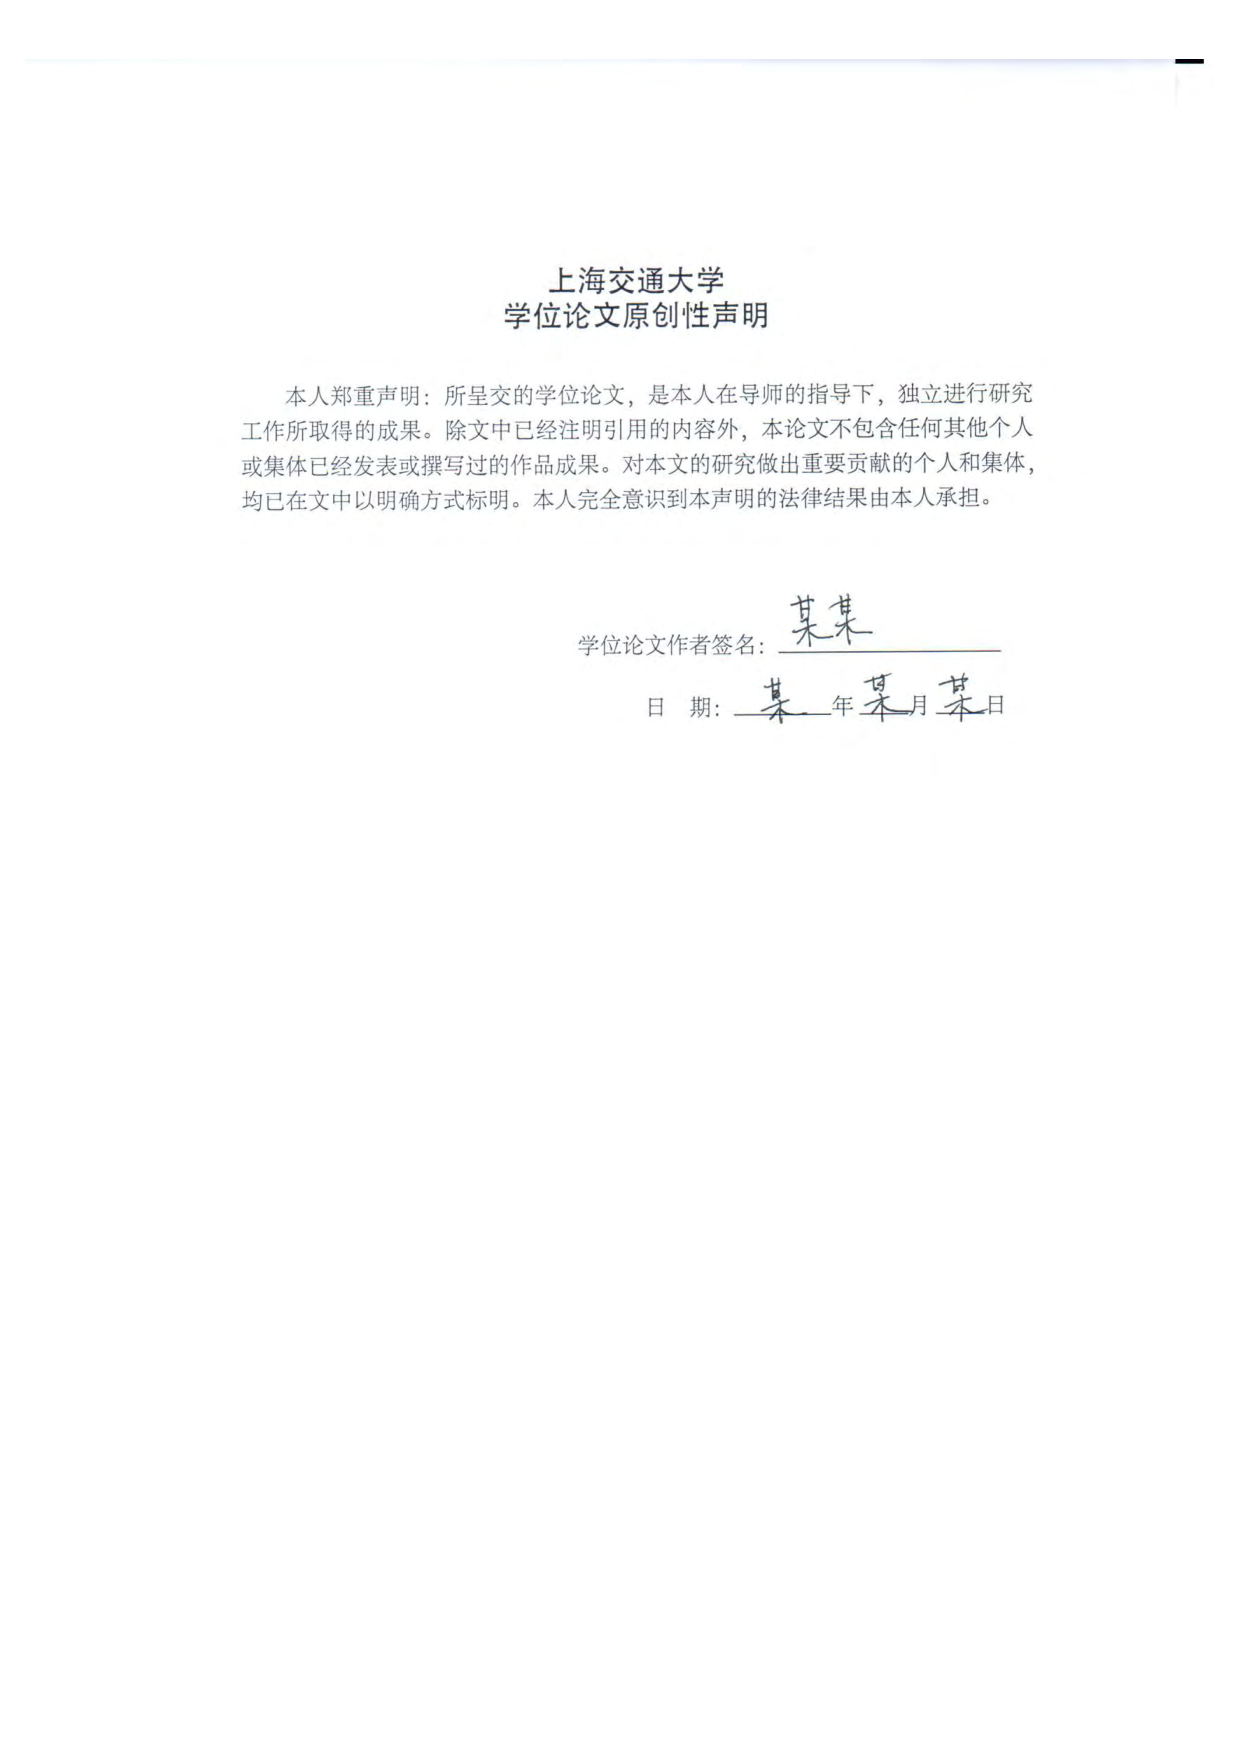
\includepdf{pdf/original.pdf}
	\cleardoublepage
	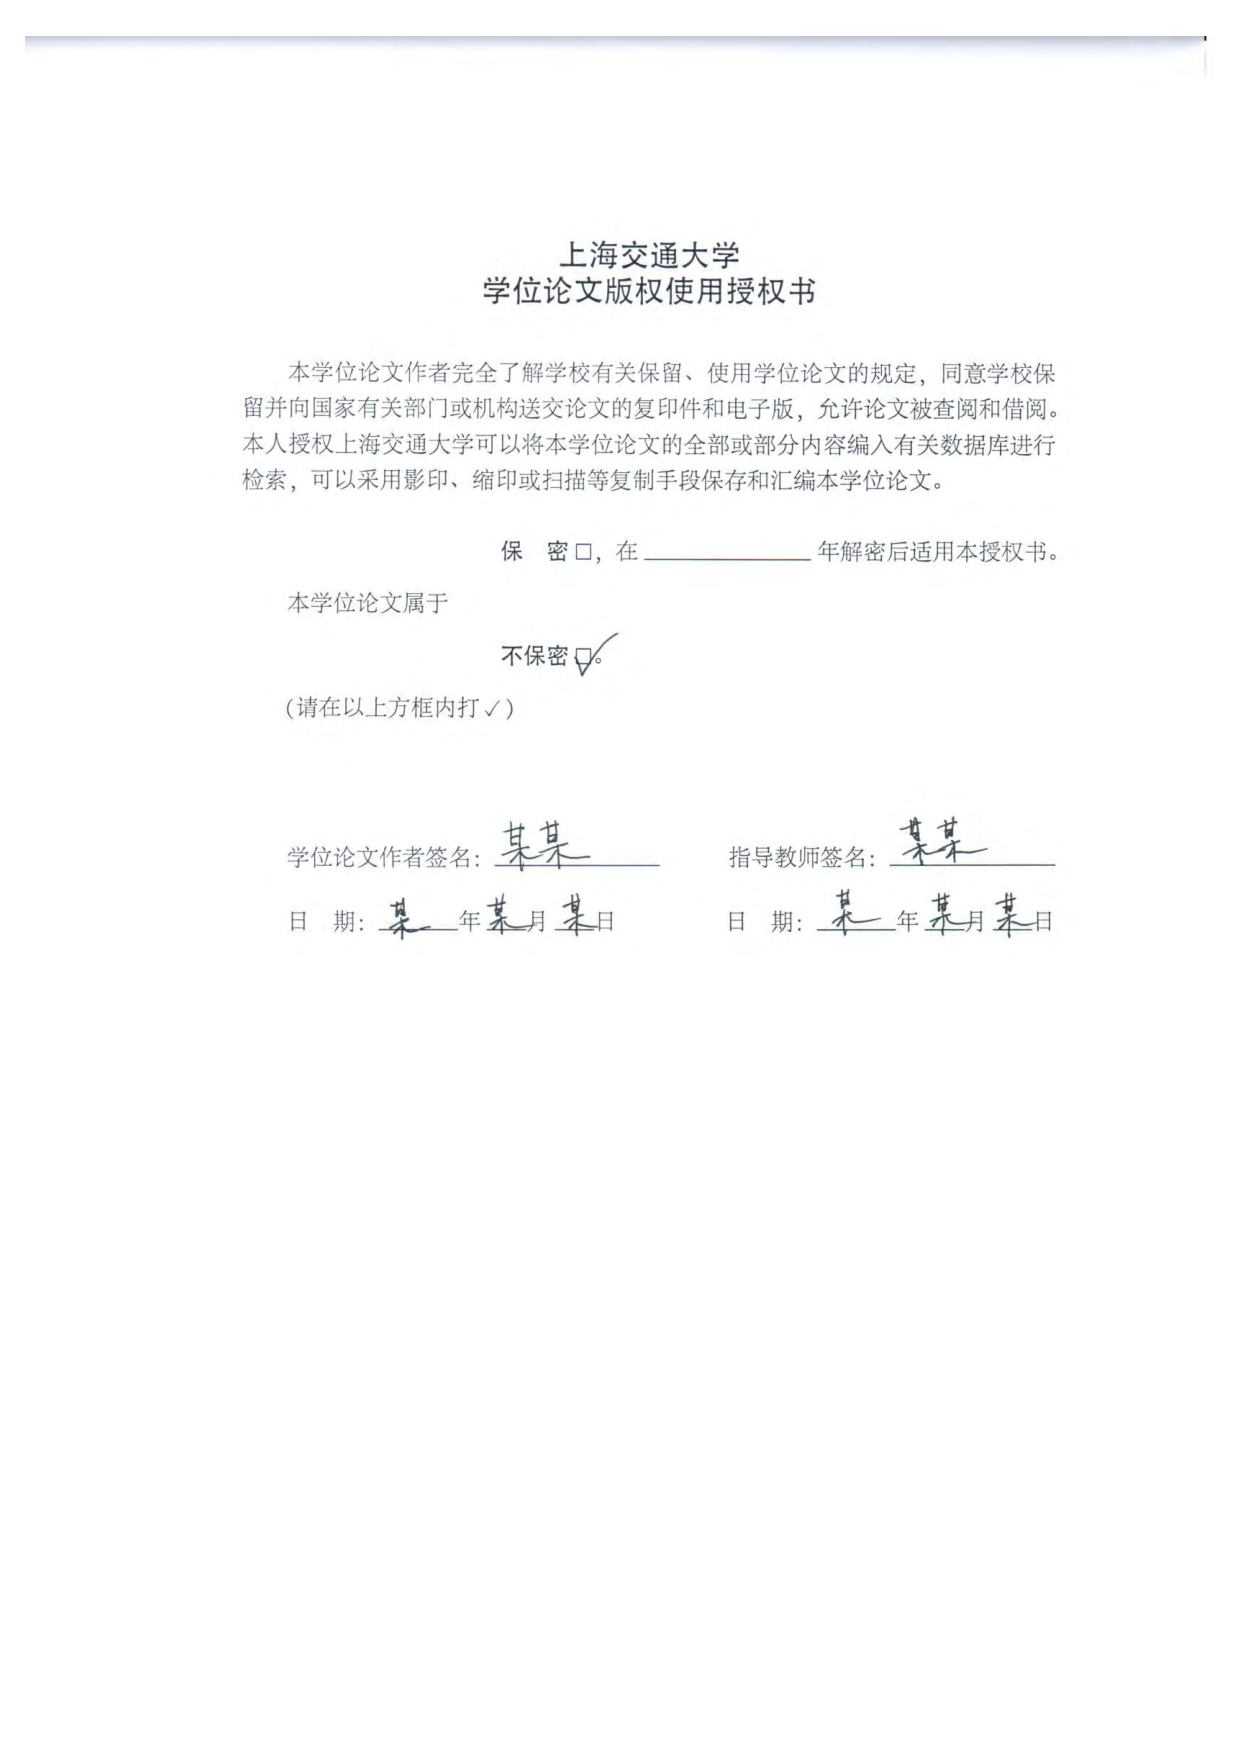
\includepdf{pdf/authorization.pdf}
	\cleardoublepage
\else
\ifsjtu@review\relax
% exclude the original claim and authorization
\else
	\makeDeclareOriginal
	\makeDeclareAuthorization
\fi
\fi
\makeatother


\frontmatter 	% 使用罗马数字对前言编号

%% 摘要
\pagestyle{main}
%# -*- coding: utf-8-unix -*-
%%==================================================
%% abstract.tex for SJTU Master Thesis
%%==================================================

\begin{abstract}
随着计算机视觉技术的不断发展,增强现实被越来越广泛地应用在娱乐、工业、医疗等各个领域。但是对于教育的应用还比较有限。教育应用的特殊性在于,用户需要自主编辑虚拟场景以满足不同的教学目的,因此需要为教育者开发一套编著系统以供他们创建个性化的实验用于教学。同时,教学的应用是非常必要的,因为学校的实验条件往往不能满足教学需要,增强现实技术可以很好的为用户提供实验指导、模拟现象等辅助信息。此外,目前的增强现实应用往往不能为用户提供触觉,交互感受有限。

本文对于增强现实应用中缺乏触感的问题,以及教学用增强现实应用对于用户要求过高两个问题提出了解决方案。通过分析、比较各类物体追踪技术和算法,本系统最终使用Ren\cite{ren2017real}的算法实现物体追踪,用户在移动真实物体的同时,可以从增强现实应用中获得虚拟图像。而对于编著系统学习成本高的问题,我们通过了解用户需求,设计、实现了用户友好的编著系统,并将它和增强现实交互进行融合。

本文设计实现了一套用于辅助教学的编著和交互系统。系统分为服务器、客户端两部分。服务器利用深度摄像头获取的RGB-D图像,采用三维符号函数描述物体并求解物体姿态,进行物体追踪。客户端基于Unity实现了编著虚拟试验的功能,并且基于Vuforia插件识别平面图像,以及算法和标定的辅助,实现虚实融合和用户交互,并且支持移动端。用户可以通过移动被追踪的物体,在手机中看到物体对应的虚拟图像。客户端和服务器之间通过Protocol Buffer进行序列化并且使用TCP/IP进行通信。

\keywords{\large 增强现实 \quad 物体追踪 \quad 编著系统 \quad 虚实融合}
\end{abstract}

\begin{englishabstract}
With the continuous development of computer vision technology, augmented reality is more and more widely used in entertainment, manufacturing, medical treatment and other fields. But the applications designed for education are still limited. The particularity of educational applications is that educators need to edit their own virtual scenes to apply in different teaching environments. Therefore, it is necessary to develop an authoring system for them to create personalized experiments for teaching. Meanwhile, the educational applications are very necessary, because the experimental conditions of the school could not meet the teaching needs sometimes, and the AR technology can provide users with auxiliary information such as experimental guidance and simulation phenomena. In addition, current AR applications often fail to provide users with a sense of touch, which limits the interaction. 

We propose a solution to the problem of the lacking in tactile sensation and the high learning costs in educational AR applications. By analyzing and comparing various object tracking techniques and algorithms, we finally use the algorithm of Ren\cite{ren2017real} to realize object tracking. Users could see virtual images from AR applications while moving real objects. As for the problem of high costs of system learning, we designed and implemented a user-friendly authoring system after analyzing user needs, and integrated it with augmented reality interaction.

This paper designs and implements a set of editing and interaction system for teaching assistance. The system could be divided into two parts: the server and client. The server uses the RGB-D image acquired by the depth camera to express the object using a three-dimensional signed function and solve the object pose function for object tracking. Based on Unity, the client implements a virtual experimentation environment. Using Vuforia plug-in, the system could identify 2D images. With the help of some algorithms and calibration operations, we realizes the fusion of virtual and real world including user -  application interaction. The client also supports mobile devices. The user can see the virtual image corresponding to the object in a mobile phone by moving the object being tracked. The client and server are serialized by Protocol Buffer and communicate with each other using TCP/IP.

 
\englishkeywords{\large augmented reality, object tracking, authoring system, virtual – real fusion}
\end{englishabstract}



%% 目录、插图目录、表格目录   【ZR注释掉了】
\tableofcontents
 \listoffigures
 \addcontentsline{toc}{chapter}{\listfigurename} %将插图目录加入全文目录
% \listoftables
% \addcontentsline{toc}{chapter}{\listtablename}  %将表格目录加入全文目录
% \listofalgorithms
% \addcontentsline{toc}{chapter}{\listalgorithmname} %将算法目录加入全文目录

% %# -*- coding: utf-8-unix -*-
\begin{nomenclaturename}
\label{chap:symb}

\begin{longtable}{rl}
$\epsilon$     & 介电常数 \\
 $\mu$ 		& 磁导率 \\
 $\epsilon$     & 介电常数 \\
 $\mu$ 		& 磁导率 \\
 $\epsilon$     & 介电常数 \\
 $\mu$ 		& 磁导率 \\
 $\epsilon$ 	& 介电常数 \\
 $\mu$ 		& 磁导率 \\
 $\epsilon$     & 介电常数 \\
 $\mu$ 		& 磁导率 \\
 $\epsilon$     & 介电常数 \\
 $\mu$ 		& 磁导率 \\
 $\epsilon$     & 介电常数 \\
 $\mu$ 		& 磁导率 \\
 $\epsilon$ 	& 介电常数 \\
 $\mu$ 		& 磁导率 \\
 $\epsilon$     & 介电常数 \\
 $\mu$ 		& 磁导率 \\
 $\epsilon$     & 介电常数 \\
 $\mu$ 		& 磁导率 \\
 $\epsilon$     & 介电常数 \\
 $\mu$ 		& 磁导率 \\
 $\epsilon$ 	& 介电常数 \\
 $\mu$ 		& 磁导率 \\
 $\epsilon$     & 介电常数 \\
 $\mu$ 		& 磁导率 \\
 $\epsilon$     & 介电常数 \\
 $\mu$ 		& 磁导率 \\
 $\epsilon$     & 介电常数 \\
 $\mu$ 		& 磁导率 \\
 $\epsilon$ 	& 介电常数 \\
 $\mu$ 		& 磁导率 \\
 $\epsilon$     & 介电常数 \\
 $\mu$ 		& 磁导率 \\
 $\epsilon$     & 介电常数 \\
 $\mu$ 		& 磁导率 \\
 $\epsilon$     & 介电常数 \\
 $\mu$ 		& 磁导率 \\
 $\epsilon$ 	& 介电常数 \\
 $\mu$ 		& 磁导率 \\
 $\epsilon$     & 介电常数 \\
 $\mu$ 		& 磁导率 \\
 $\epsilon$     & 介电常数 \\
 $\mu$ 		& 磁导率 \\
 $\epsilon$     & 介电常数 \\
 $\mu$ 		& 磁导率 \\
 $\epsilon$ 	& 介电常数 \\
 $\mu$ 		& 磁导率 \\
 $\epsilon$     & 介电常数 \\
 $\mu$ 		& 磁导率 \\
 $\epsilon$     & 介电常数 \\
 $\mu$ 		& 磁导率 \\
 $\epsilon$     & 介电常数 \\
 $\mu$ 		& 磁导率 \\
\end{longtable}

\end{nomenclaturename}
 % 主要符号、缩略词对照表

\mainmatter	% 使用阿拉伯数字对正文编号

%% 正文内容
 \pagestyle{main}
 \chapter{绪论}
\label{chap:myIntro}

\section{研究背景及意义}
\label{sec:background}
增强现实(Augmented Reality,AR)是一种利用计算机生成视觉、听觉等感官信息,然后与真实世界中的物体进行混合,最终呈现在用户面前的技术。\cite{ARconception}

目前增强现实在很多领域都有使用,例如在游戏领域,增强现实技术可以改变传统游戏的交互方式,为玩家提供更加新奇的游戏体验。
    
\begin{figure}[!htp]
  \centering
  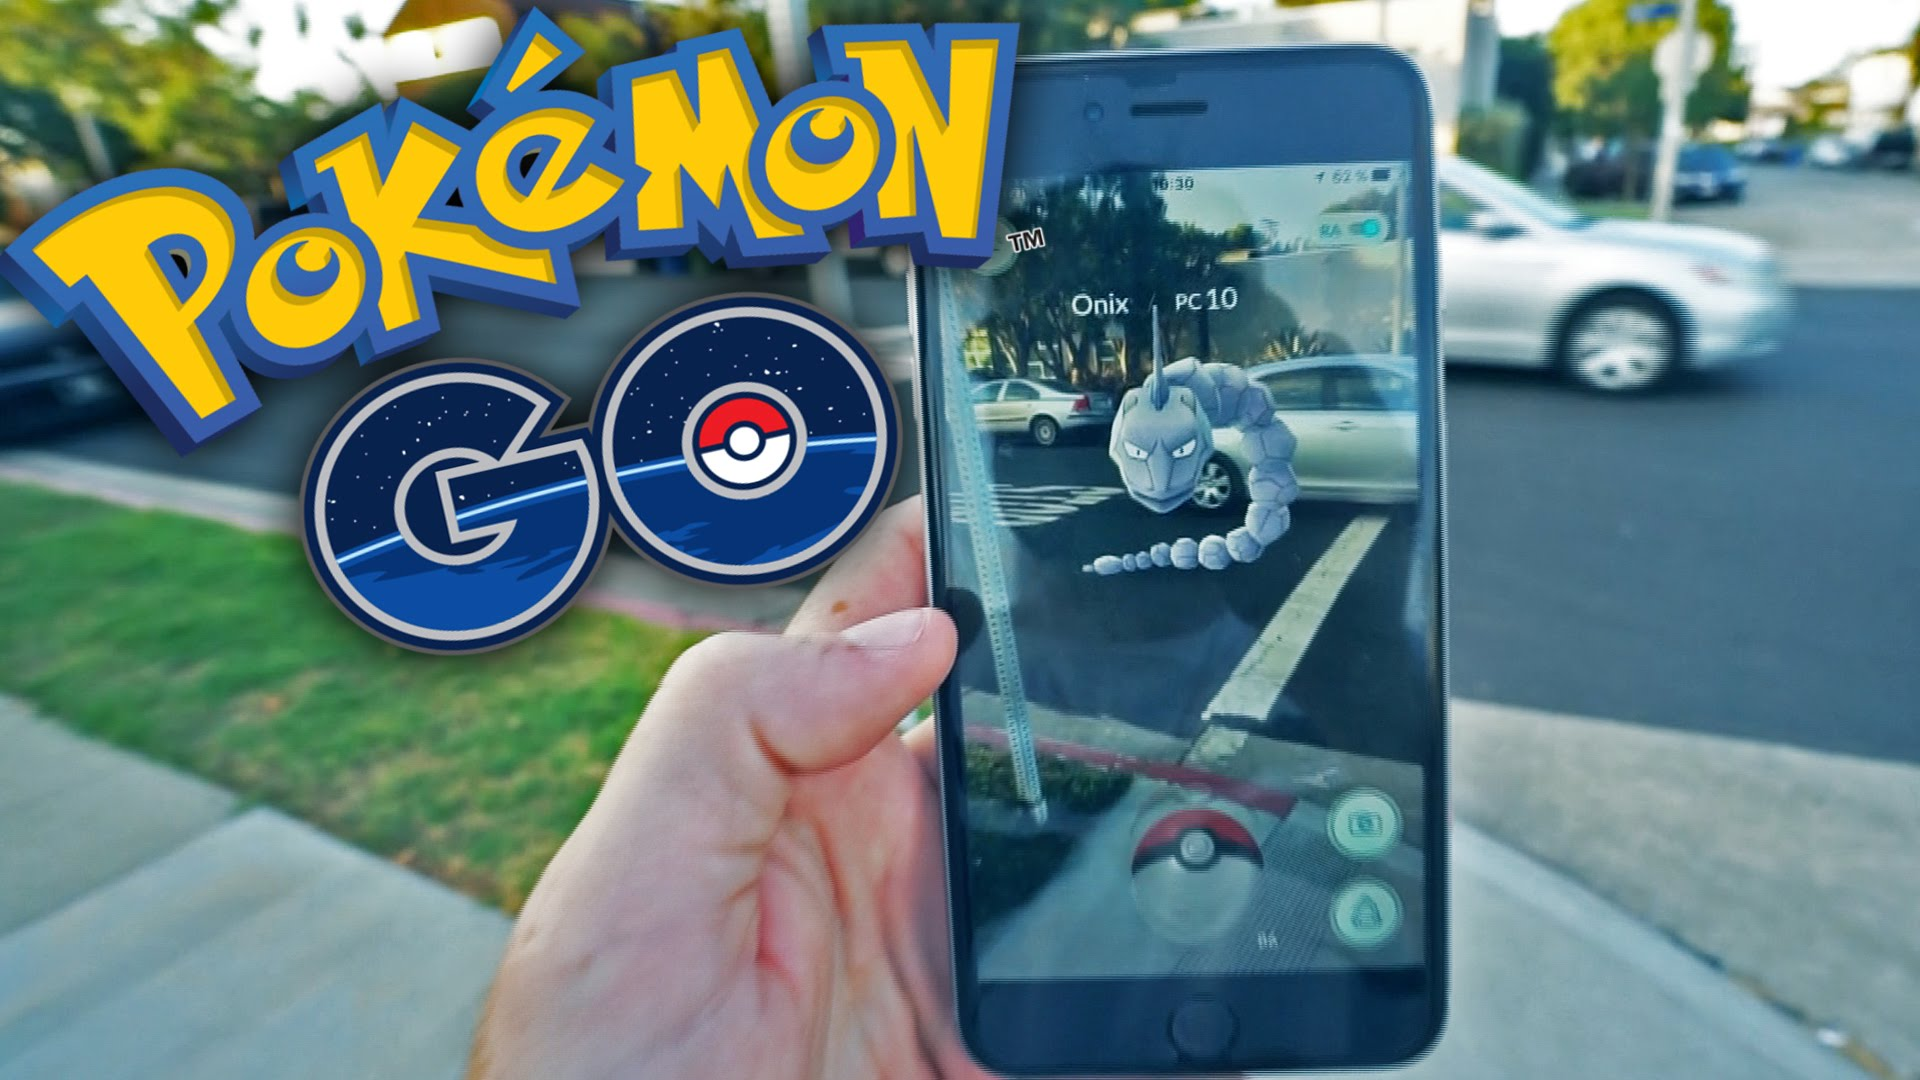
\includegraphics[width=12cm]{pokemongogaming.jpg}
  \bicaption[AR游戏 Pokemon Go海报]
    {AR游戏 Pokemon Go海报}
    {The wallpaper of AR game Pokemon Go}
 \label{fig:longcaptionbad}
\end{figure}

在实际应用中,增强现实也被广泛应用于提供辅助信息。例如在汽车领域,增强现实技术能够在驾驶过程中为驾驶员提供导航、路况提醒等信息。\cite{ARdriving}在医学领域,可以通过AR技术将超声波图像显示在患者身体上为医生提供更多信息。\cite{billinghurst2002augmented}

增强现实技术也逐渐被应用在教育领域,为教师和学生提供更加丰富的教学内容。目前的实验教学存在诸多问题,例如,实验条件(器材、空间、教师、开放时间)有限,学生动手操作和试错的机会少,实验指导不能随着实验进行实时提示与更新等问题。而增强现实技术因为可以可视化抽象概念,模拟复杂的现象,提供模拟实验练习等优势,因此被广泛应用。\cite{wu2013current}但是,教育领域与上述其他领域不同的是,用户(教师)也是软件开发的一部分,需要具有自主编辑实验的自由。但是教师由于通常不具备软件开发能力,因此需要应用提供一套用户友好的编著系统。

与此同时,处于为用户提供更丰富的交互体验,例如为用户提供触觉,或将显示信息与可交互的物体进行更好融合的目的,增强现实应用往往需要的实现对于物体的识别和追踪。

本文旨在开发一套增强现实辅助教学应用,在后端通过物体追踪,为用户提供具有真实触感的交互体验,并且在交互过程中显示物体的辅助信息。在前端开发一套用户友好的编著系统,为非计算机专业人士编辑用于教学的增强现实应用。

这套系统的意义在于,教育者可以在花费较少的学习成本的前提下,自主创建、编辑实验,并且结合现实器材,为学生提供多样的模拟实验。在教学过程中,教育者减少了教学、演示、实验指导的负担,学生实验可以不再受器材、人员等因素的限制,在保证安全的同时有大量误操作、试错的机会,可以更好的学习实验。而与增强现实技术相结合,该系统可以使学生拥有多种感官的体验,模拟实验更加逼真。



\section{国内外研究现状}
\subsection{物体追踪}
在增强现实应用中,出于融合需要,往往需要对真实物体进行物体姿态检测和追踪。目前很多学者在这方面做出了研究。基于模型的物体追踪可以分为两类,基于RGB-深度图像和仅基于RGB图像。

对于基于RGB图像进行物体姿态检测的研究,目前使用较多的、可以达到实时效果的是基于模式匹配(template matching)的方法。例如Hinterstoisser等人提出的LINE方法\cite{hinterstoisser2011gradient},在传统的使用图像和梯度(gradients)检测物体的模式匹配方法的基础上,通过依靠局部优势梯度方向(local dominant gradients orientation)建立模式不变量,并且考虑梯度方向在图片中的相邻区域。通过上述两者结合来数学表示输入图像,之后进行模式识别,可以获得更加稳定和高效的追踪效果。此外,近年来也有一些基于学习的方法进行物体姿态检测的研究被提出。例如,Brachmann等人提出的,基于随机森林(random forest)扩展的方法。\cite{brachmann2016uncertainty}但是由于选择的特征会在很大程度上影响决定姿态的投票数量,基于随机森林的方法在性能上往往并不能达到实时的要求。

而对于基于RGB图像进行物体追踪的方法来说,最早能够够达到实时要求的是算法是Prisacariu和Reid提出的PWP3D算法\cite{prisacariu2012pwp3d}。该算法构建了一个概率框架,将前景部分使用符号距离函数进行描绘,并且定义了该区域的能量。而后景部分则基于像素级别的后验隶属概率进行描绘。之后这个方法被Hexer等人发展为利用局部颜色直方图进行前后景分隔,提升了效率。\cite{hexner20162d}

但是仅使用RGB图像进行物体追踪的技术相比于添加深度图像进行辅助仍然有所欠缺。例如LINE方法\cite{hinterstoisser2011gradient}在有深度信息的时候,可以通过获得物体的表面法向量来进一步提升鲁棒性。而Brachmann的方法\cite{brachmann2016uncertainty}也通过边缘化物体坐标分布的深度值,从而弥补深度值的缺失,实现追踪。相比之下,结合深度值的方法则更加成熟与稳定。

在物体检测方面,传统的方式可以分为基于模式和基于特征两种。上述的基于模式匹配的LINE方法\cite{hinterstoisser2011gradient}在加入深度信息辅助,以及其他的类似方法\cite{kehl2016hashmod, rios2013discriminatively}, 都可以实现基于RGB-D图像的物体检测。但是这些方法在检测多个物体的时候计算率都是呈线性增长的,可扩展性较差。而基于特征的方法,最早是通过RGB图像获得特征\cite{lowe2004distinctive},然后反向投影到三维坐标中的\cite{lowe2001local}。在三维描述符引入后,则可以直接通过三维点云计算特征点\cite{mian2010repeatability}。从而获得比较好的延展性,但这些方法的性能往往并不能达到实时的要求。在机器学习发展之后,出现了基于随机森林投票确定物体姿态的方法。\cite{brachmann2016uncertainty, tejani2014latent}前者是使用能量函数进行姿态估测,而后者则是使用投票机制。在这之后,也出现了基于卷积神经网络(convolutional neutral network, CNN)进行姿态识别的研究\cite{kehl2016deep}.该方法使用了局部取样的RGB-D图像补丁(patch)进行神经网络训练,然后在使用的时候通过补丁描述符进行匹配推测物体姿态。

而在物体追踪方面,目前的方法大多数都是基于已知待追踪模型的数据的。他们通过构造图像的函数,描绘观测图像和目标图像之间的差别,将构造函数最小化从而确定物体姿态。一种处理图像数据的方式是迭代最近点算法(iterative closest point, ICP)。他的目的是通过找到待配准点云数据(追踪时获取的数据)与参考点云数据(物体模型数据)之间的旋转和平移关系,进行最优匹配。Held实现的物体追踪算法就使用了这个方法。\cite{held20123d}但是在多物体追踪时候往往需要进行预分隔,必须使用一个不同的模型,在应对多物体的时候效果并不好。
另一种替代ICP的方法是符号距离函数(Signed Distance Function, SDF)。他描绘了点云和物体模型的关系。本文实现的物体追踪系统使用了Ren等人基于SDF实现的物体追踪算法。\cite{ren2017real}他们通过描绘物体的SDF函数,构造代价函数,求解物体姿态。具体算法将会在相关技术中详细分析。

\subsection{虚拟场景中的编著系统}
目前针对用户自主编辑虚拟场景的需求,有许多应用面市。例如基于互联网交互游戏Second life的编程语言Linden Scripting Language(LSL),是用户·可以·通过简单的编程,就可以实现在虚拟场景中自定义与其他物体的交互。\cite{LSLTutorial}在此基础上,也有很多应用,方便用户进行简单的编程之后生成代码导入second life,如Particle,Dialog Menu, MiceOnABeam Visual Scripting Tool等等。\cite{zhong2014domain}这些工具虽然便利了用户使用虚拟场景,但是仍然需要用户具备一定的编程能力,距离实际教师教学仍有一定差距。

在这之后,有许多虚拟场景中的模拟程序被开发,例如Ying Zhong等人开发的化学模拟实验引擎。\cite{zhong2014domain}用户可以创建、编辑、操纵化学实验用具,通过·TCP/IP与服务器和数据库联通。工具具有比较好的易用性,但是体现化学专业知识、进行操作提示的部分比较少,交互方式也比较局限,并且只局限在PC端。此外,牛津大学也开发了一款用于教学的化学实验模拟引擎,虽然引擎本身对于化学实验及其原理、实验操作都有比较详细的讲述,但是由于演示使用过视频片段整合形成的,交互方式非常局限。\cite{OxfordChe}在这之后,Ali等人开发了一套化学实验模拟引擎系统,\cite{ali2014effect}将上述两者整合起来,既支持比较多的交互方式,还支持化学知识的教学。除此以外,虚拟场景编辑也应用在了物理等其他自然科学领域。\cite{daineko2017using}

虽然编著系统已经有广泛的应用,但是从上述软件可以看出,交互方式仍然局限在电脑屏幕,而且对于实验环境的编辑也比较缺乏。

\section{本文主要工作}
本文开发了一套增强现实应用,前端基于Unity引擎开发,为教育者提供了一个可以创建实验、调节实验环境的编著系统,后端通过Kinect获取RGB-D图像,基于上述的Ren提供的算法\cite{ren2017real}实现对特定模型的追踪,并结合Vuforia工具辅助,在Unity场景中渲染,从而达到虚实融合,具有真实触感的增强现实应用。


\section{本文结构}
本文一共分为七章。
\begin{itemize}[noitemsep,topsep=0pt,parsep=0pt,partopsep=0pt]
\item 第一章概括介绍了目前增强现实应用的发展背景,以及关于物体追踪和编著系统的研究状况,并简单介绍了项目特点。
\item 第二章着重介绍了项目是使用到的技术以及算法。主要包括物体追踪以及相应的软硬件工具以及理论,编著系统实现过程中使用到的技术以及引擎,上述两者通信的时候使用的框架和协议等。
\item 第三章分析了项目需求,并结合项目需求进行项目功能设计。
\item 第四章从实现角度介绍了项目的系统架构,包括前端的编著系统架构、后端的物体追踪系统架构、以及两者之间通信的架构。
\item 第五章着重从代码层面讲述系统实现。
\item 第六章简要介绍系统实现的效果,并分析了网络传输和物体追踪的性能,并且分析了编著系统和易用性、增强现实应用的使用体验等。
\item 最后一章总结全文,并且给出项目存在的优缺点,给出项目未来发展方向。
\end{itemize}

 \chapter{相关技术}
\label{chap:tech}

本系统涉及到了物体追踪、编著与交互系统以及它们之间的通信三部分。物体追踪的实现主要使用了Ren的LibISR工具库\cite{Ren_3DV_2014,star3d_iccv_2013}。为了适配该工具库,需要通过硬件分别获取Kinect的彩色图像和深度图像,进行融合从而获取准确的RGB-D图像,因此需要对使用的Kinect 2进行标定和驱动。标定使用了ROS系统中的Kinect标定工具iai-kinect\cite{iai_kinect2},并且将标定结果进行再加工获得RGB图像与深度图像的映射关系。驱动则使用了开源工具Libfreenect2\cite{libfreenect2}。编著与交互系统基于Unity引擎\cite{Unity}进行了实现,同时使用了Vuforia插件\cite{Vuforia}实现基于增强现实的交互,以及Android SDK\cite{Android}实现移动端的使用。通信则使用了Protocol Buffer\cite{Protobuf, ProtobufNet}串行化数据结构,然后通过TCP通信进行传输。本章将详细介绍上述技术或工具,以及如何将它们应用在本系统当中。

\section{物体追踪相关技术}
\subsection{Kinect驱动}
Kinect是一款微软开发的硬件设备,主要有彩色摄像头,以及红外线发射器和红外线CMOS 摄影机所构成的3D结构光深度感应器。该产品最初被应用于体感游戏,目前则主要被学界用来获取RGB-D图像。本系统使用了Kinect的第二代版本,具有更高的分辨率和性能,但是与第一代相比,他的彩色图像与深度图像分辨率并不成比例,因此在图像使用的过程中需要更多的处理。例如,在进行图像显示的时候,使用相同分辨率的窗口,往往会看到彩色图像和深度图像有不同程度的扭曲。

微软官方提供了Kinect SDK,但是只支持windows系统。此外,还有一些非官方、开源的Kinect驱动。OpenNI\cite{Openni}也提供了开源的对于Kinect传感器的支持,但是目前已经停止更新了,对于Kinect2的支持比较差。此外,还有基于ROS系统的iai kinect\cite{iai_kinect2}可供使用。本系统使用的是libfreenect2\cite{libfreenect2},它基于openni实现,但是对于Kinect2具有比较好的支持。

\subsection{LibISR物体追踪工具}
LibISR是Ren等人基于三维符号距离函数(3D Signed Distance Function )实现的工具库\cite{Ren_3DV_2014, star3d_iccv_2013}。本项目目前只用到了追踪单个物体的部分,这一小节将针对系统中单个物体追踪的算法进行介绍\cite{ren2017real}。

该项目的追踪流程如图\ref{fig:model}所示,首先相机将物体空间下的点映射到相机空间,并且在相机平面成像。该工具在获得相机的RGB-D图像之后,通过前后景分析,将像素分类并反向映射(back-projection)到物体空间,通过他们在物体空间的三维符号函数,得到代价函数,并求出使代价函数局部最小化的解从而还原出物体姿态。

\begin{figure}[!htp]
  \centering
  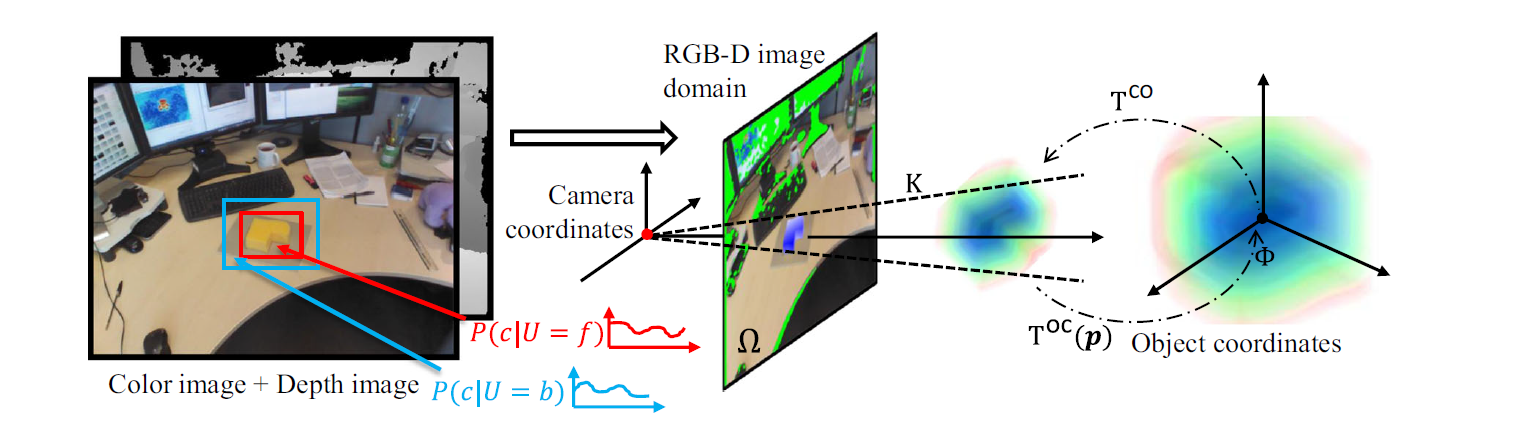
\includegraphics[width=14cm]{figure/model.png}
  \bicaption[LibISR物体追踪流程示意图]
    {LibISR物体追踪流程示意图\cite{ren2017real}}
    {The Flow Diagram of LibISR Tracing Object }
 \label{fig:model}
\end{figure}

LibSIR使用的生成模型(generative model)如图\ref{fig:Gmodel}所示。

\begin{figure}[!htp]
  \centering
  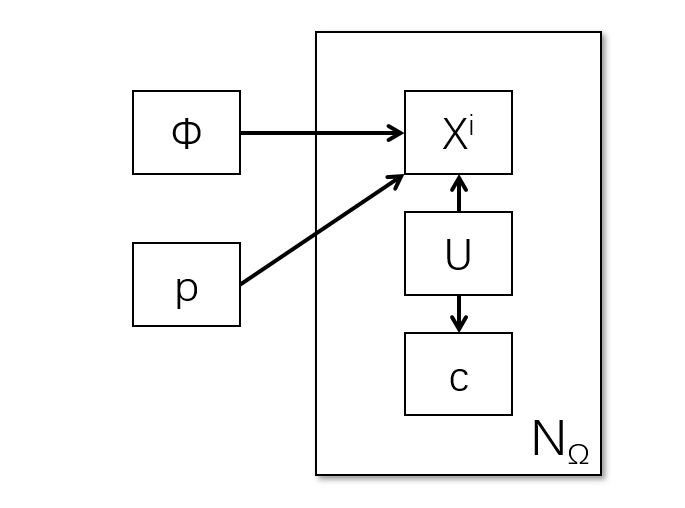
\includegraphics[width=6cm]{figure/jointModel.png}
  \bicaption[LibISR单物体追踪生成模型]
    {LibISR单物体追踪生成模型\cite{ren2017real}}
    {The Generative Model of Tracing Single Object}
 \label{fig:Gmodel}
\end{figure}

其中$p$表示物体的姿态,$\Phi$表示物体的形状。$N_\Omega$表示输入图片中所有像素的集合,$X^i$代表了每个像素的深度值,而$c$代表像素的RGB值。$U$是一个潜变量(latent variable),代表该像素点是前景或后景部分。其中的箭头表示变量之间的依赖关系。

利用上述的生成模型可以估计出联合概率分布(joint probability distribution):
\begin{equation}
 P(X^i, c, U, \Phi, p) = P(\phi)P(p)P(X^i|U, \Phi, p)P(c|U)P(U)\label{L1}
\end{equation}
将公式(\ref{L1})对变量$U$进行边缘化,可以得到公式:
\begin{equation}
 P(X^i, c, \Phi, p) = P(\phi)P(p)\sum_{u\in\{f,b\}}P(X^i|U=u, \Phi, p)P(c|U=u)P(U=u)\label{L2}
\end{equation}

由于图像空间下的坐标点可以通过输入的RGB-D图像以及相机的标定参数反向映射到相机空间,又可以通过物体的姿态信息反向映射到物体空间,因此图像空间的点可以与物体空间的点一一对应,因此可以使用关于物体空间下的函数,即3D SDF函数,描绘图像空间的概率分布。
\begin{equation}
 P(X^i|U=f, \Phi, p)=\delta^{on}(\Phi(X^O))/\eta_f\label{L3}
\end{equation}
\begin{equation}
 P(X^i|U=b, \Phi, p)=H^{out}(\Phi(X^O))/\eta_b\label{L4}
\end{equation}
其中
\begin{equation} \label{L5}
 \delta^{on}(\Phi)=sech^2(\Phi/2\delta) \quad\mathrm{,}\quad
 H^{out}(\Phi)=
 \begin{cases}
    1-\delta^{on}(\Phi) &\Phi\geq0\cr
    0 &\Phi<0
\end{cases}
\end{equation}
\begin{equation}\label{L6}
 \eta_f=\sum_{j=1}^{N_\Omega}\delta^{on}(\Phi(X_j^O))
\quad\mathrm{,}\quad
 \eta_b=\sum_{j=1}^{N_\Omega}H^{out}(\Phi(X_j^O))
\end{equation}
则前后景模型的先验概率可以用公式(\ref{L7})表示
\begin{equation}\label{L7}
 P(U=f)=\eta_f/\eta \quad\mathrm{,}\quad  P(U=b)=\eta_b/\eta \quad\mathrm{,}\quad  \eta=\eta_f+\eta_b
\end{equation}
将公式(\ref{L3}) - (\ref{L7})带入公式(\ref{L2})可以得到对于每一个单独的像素来说,它的联合概率分布为
\begin{equation}\label{L8}
 P(X^i, c, \Phi, p) = P(\phi)P(p)(P(c|U=f)\delta^{on}(\Phi(X^O)) + P(c|U=b)H^{out}(\Phi(X^O)))
\end{equation}

在追踪的时候需要使用RGB-D图像和物体模型数据,通过最大后验概率估计物体姿态。在每个时刻的物体姿态相互独立的基础上,通过条件概率公式可以得到:
\begin{equation}\label{L9}
argmax_{p_t}P(p_t|\Phi,\Omega_t) = argmax_{p_t}\frac{P(p_t,\Phi,\Omega_t)}{P(\Phi,\Omega_t)}
\end{equation}
由于图像中的每个像素都是彼此独立的,因此可以得到
\begin{equation}\label{L10}
P(p_t,\Phi,\Omega_t)=\prod_{j=1}^{N_\Omega}P(X_j^i, c_j, \Phi, p)
\end{equation}
而物体用三维距离函数描绘的物体模型$\Phi$和图像$\Omega$之间也是相互独立的,因此将公式(\ref{L8})和公式(\ref{L10})带入(\ref{L9})可得
\begin{equation}\label{L11}
P(p_t|\Phi,\Omega_t) \sim \prod_{j=1}^{N_\Omega}\Big\{P(c|U=f)\delta^{on}(\Phi(X^O)) + P(c|U=b)H^{out}(\Phi(X^O))\Big\}
\end{equation}
将公式(\ref{L11})求负对数可以得到用于计算的代价函数了
\begin{equation}\label{L12}
\mathscr{E} = -\sum_{j=1}^{N_\Omega}log\Big\{P_j(c|U=f)\delta^{on}(\Phi(X^O)) + P_j(c|U=b)H^{out}(\Phi(X^O))\Big\}
\end{equation}

在最小化该代价函数的过程中,使用了Levenberg–Marquardt算法。该算法通过不断的迭代,搜索出使非线性函数局部最小的数值解。该算法在每一次迭代的过程中计算
\begin{equation}\label{L13}
p^*=\Big\{-[J^TJ + \lambda diag[J^TJ]]^-1\frac{\partial\mathscr{E}}{\partial p^*}\Big\}
\end{equation}
其中$J$是Jacobian矩阵,$\lambda$是算法的惩罚因子,它会在每一次迭代的过程中发生调整。$p^*$是姿态的变化量,通过三维的位移向量和三维旋转向量进行表示。
由公式(\ref{L13}),在每一次迭代之后,将计算出的姿态变化量应用于上一次迭代的姿态结果之上,直到计算出最终的该帧内的姿态变化,并将它应用到上一帧的最终姿态就可以得到物体的变化后的姿态了。
在每次迭代之后,如果将图像空间的点使用姿态信息反向映射到物体空间,会发现具有前景概率大于后景概率的点,会在SDF的影响下不断向物体表面移动,而后景概率较大的点则会不断远离物体,最终得到理想的结果。
由于前后景概率模型对于系统的鲁棒性非常重要,系统会在每帧使用最贴合物体表面,即3D SDF函数值较接近0的点,更新物体的前景概率模型,同时使用目标区域附近的点更新后景模型,以达到更好的效果。其公式为
\begin{equation}
P_t(c|U=u)=(1-p^u)P_{t-1}(c|U) + p^uP_{t-1}(c|U)
\end{equation}
其中$u$为实验得到的参数。

在使用该系统进行物体追踪的过程中,可以发现,单个物体可以在抖动、旋转的过程中仍然具有比较好的追踪效果。但是从本质上讲,使用RGB-D图像对于相机标定的效果,即RGB图像和深度图像的融合效果有比较高的要求,标定的质量很大程度上决定了追踪的效果。此外,受硬件限制,当深度摄像头暴露在强光条件下,也会影响物体追踪的效果。另一方面,从该算法的角度讲,由于物体的姿态、前后景模型都是基于前一次数据累积的,因此当发生追踪错误的时候,追踪误差往往也会累积,影响前后景区分模型,最终很难恢复正确的追踪。

\subsection{CUDA}
上述用于物体追踪的工具LibISR,以及用于驱动Kinect的Libfreenect 2都使用了CUDA\cite{CUDARef}(Compute Unified Device Architecture,统一计算设备架构)进行计算加速。CUDA是由Nvidia公司推出的一套并行计算平台和应用编程接口(API)。用户可以通过CUDA访问GPU的指令集架构(instruction set architecture,ISA),控制显卡中的并行运算模块,提升并发运算速度。由于GPU本身存在很多核心,线程是轻量级的,非常适合进行密集计算任务,例如在图像追踪中就可以用于图像和矩阵的计算。

虽然CUDA基于GPU进行运作,但是实际应用中需要GPU与CPU协同配合。CPU被称为主机端(host),GPU被称为设备端(device)。通常的使用流程是,首先为主机端分配内存,初始化数据。然后将数据复制到设备端,设备端进行运算,运算结束后,将结果复制回主机端,完成任务。GPU中并行执行的函数被称为内核(kernel)。在内核启动GPU进行运算前,必须预先设置GPU的线程结构,包括指定内核的网格(grid)结构,以及每个网格包含的线程块(block)的结构。他们的关系如图\ref{fig:ceda}所示。

\begin{figure}[!htp]
  \centering
  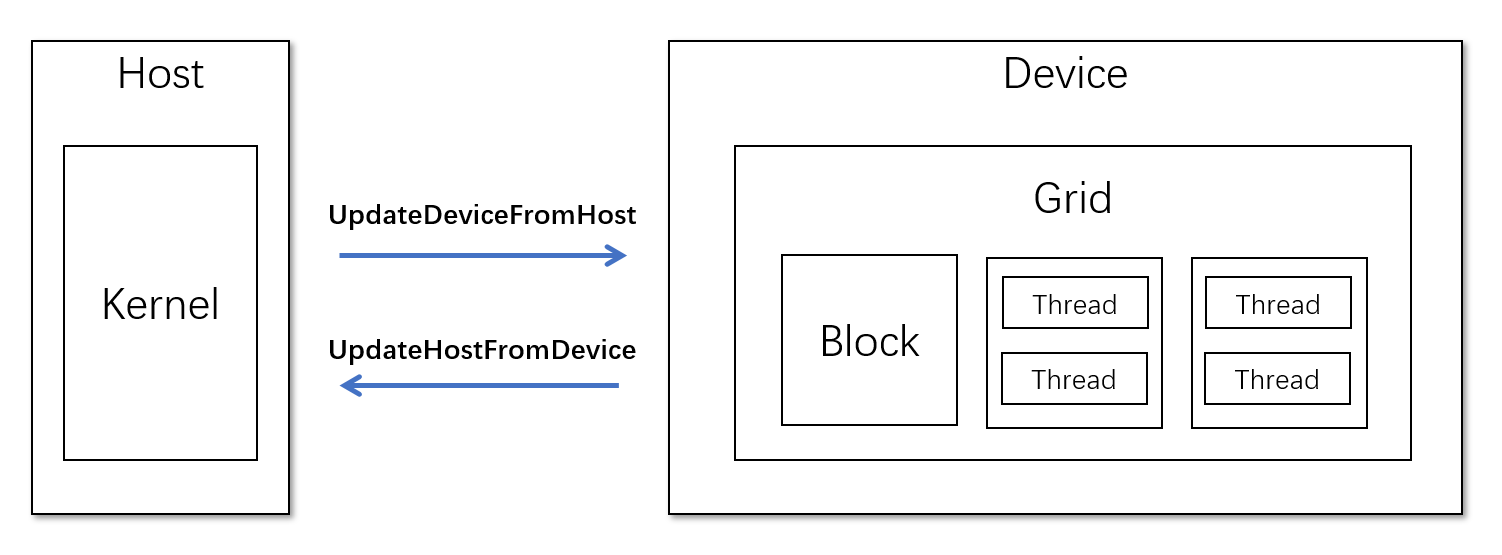
\includegraphics[width=12cm]{cuda.png}
  \bicaption[Kernel上的两层线程组织结构]
    {Kernel上的两层线程组织结构}
    {The Double-Layer Kernel Architecture }
 \label{fig:ceda}
\end{figure}

由图\ref{fig:ceda}可见,通过Block ID和Thread ID就可以唯一的确定一个线程了。而这两个变量也是thread在运行时自己可以直接访问的变量。因此,可以通过它们进行图片或矩阵的遍历和并发。

\section{编著与交互系统相关技术}
面向于教育者的编著系统基于Unity引擎开发,除引擎本身提供的基本功能之外,还使用了Android SDK、Vuforia等插件。本小节将对这些技术进行介绍。

\subsection{Unity引擎}
Unity\cite{Unity}是一款由Unity Technologies开发的引擎。引擎最初是一款针为Mac OS X进行开发的游戏引擎,目前已经扩展至Windows、Android、Play Station、AR、VR等诸多平台,同时仍然保持着轻量级的特点。此外,Unity开发的软件也从最初的游戏,发展为汽车、制造、电影动画、建筑等诸多领域的应用。

Unity项目现在通常基于C\#语言进行开发,以下将对本系统中使用的Unity功能进行介绍。
	
UI方面,Unity提供了按钮、下拉框、文本输出框、选择框等等控件。这些控件可以通过设置画布的自动缩放模式,以及锚点的控制,实现对于不同分辨率的自适应。此外,当这些控件的状态发生变化时,可以触发相应的事件从而控制应用中的游戏对象。除上述控件之外,Unity也可以获取用户的鼠标、键盘事件。对于鼠标的点击事件,在移动端可以自动转换为手指的点击事件,从而减轻了跨平台项目对于代码修改的负担。

游戏控制方面,使用了Game Manager的概念。一般的物体会在应用场景切换的时候被销毁掉,但是Game Manager不会,可以通过它储存信息,并且控制场景切换流程,是一些重要信息在场景切换之后仍然保存。

在基于增强现实交互的过程中,unity会在获得物体的追踪结果之后,在场景中的虚拟物体进行相应的位移、旋转,并最终覆盖在手机的摄像画面上,这是本系统实现增强现实交互的基础。

此外,Unity还提供了控制场景光照、物体材质与着色器、物理模拟与碰撞检测等等功能,都在本项目中有所应用。

\subsection{Android SDK}
Android SDK\cite{Android}是Google开发的提供给Android应用开发人员的软件开发工具包(Software Development Kit,SDK)。对于Unity开发的应用来说,如果需要在Android平台上运行,就需要安装SDK,使Unity可以将项目以Android的架构进行构建(build),以APK的格式发布。

\subsection{Vuforia}
Vuforia\cite{Vuforia}是一款主要基于移动设备,用于实现增强现实应用的软件开发工具包。Vuforia通过摄像头,获得场景图象,然后使用计算机视觉的方法,结合标志物(marker),实现识别、追踪目标物体,最后通过Unity将虚拟物体渲染在手机屏幕的对应位置上。用户通过手机屏幕,就可以看到真实场景与虚拟画面相融合的效果了。
	
对于融合精度要求不高的应用,例如目前市面上多数增强现实游戏,虚拟物体与真实物体并不存在很强的联系。这种情况下,应用往往只需要空间中的任意一点,或是识别出一个可以搭建虚拟场景的平面就可以开始游戏了。一种被广泛应用的增强现实工具是Vuforia Ground Plane\cite{VuforiaGround},用户在开始使用的时候,通过摄像机获取场景信息,然后选定一个理想的平面,虚拟图像就可以以该平面为游戏场景进行绘制了。但是平面识别存在着精度差等问题。当摄像机相对于场景进行移动之后,标记平面的锚点很容易发生偏移,特别是在初始化的平面被摄像头放大、被其他物体遮挡遮挡,或被移出摄像机空间的情况下。

为了提高精度,往往需要在场景或被追踪的物体上添加标志物。目前,Vuforia支持追踪标志物类型包括单张图片(二维码)、立方体、圆柱体或圆台、任意的三维模型四种。用户需要在Vuforia官网获取许可(license),然后使用官网的数据库导入标志物数据,并且在应用中使用对应的许可和数据库,就可以实现相应物体的追踪了。
	
比较常用的是平面标志。平面标志通常由具有一定特征的图片或者二维码组成。Vuforia图片识别的原理是,用户将标志物图片上传后,服务器会将上传的图片转为灰度图,提取其中特征点,打包保存在数据库中。在实时检测的时候,Vuforia会将场景中的图像特征点与数据库中的模板图片特征点数据进行匹配。被用于识别的图片也具有一定的要求,首先需要具有比较高的对比度,而且重复度比较低。被上传到官网的图片的8\%宽度被称为功能排斥缓冲区,该区域并不会被识别。Vuforia还会对上传的图片进行评级,通常带有分明轮廓,棱角分明的图片评级比较高,追踪效果也会比较好。综上所述,二维码非常符合上述条件,所以它本身就是一种非常好的识别标识物。

由于平面标志本身具有位置和尺寸信息,应用可以通过标志物确定出比较准确的物体位置,即使标志物被遮挡或离开相机范围,在标志物返回视野的时候,仍然可以精准的定位。此外,通过计算机视觉识别平面标志的计算效率也比较高。但是平面标志也具有一定的缺点。首先由于平面标志的特性,只有在标志与相机平面平行的时候才有比较好的追踪效果,因此难以追踪可以在三维场景中自由移动的物体。实践证明,当平面标志与相机平面具有一定的倾角的时候,虽然仍然可以识别出倾角,但是可能会发生产生歧义。此外,将平面标志固定在被追踪的物体上,从而保持平面标志与被追踪物体相对静止,往往会影响用户移动物体,而且很容易发生遮挡。因此,平面标志往往被应用于静态的增强现实场景,而很少用于物体追踪。

除了平面标志外,也可以使用三维的标志,如圆柱体,立方体,甚至任意的三维模型等等。通过这些三维标志,物体可以在三维场景中移动时具有比较好的追踪效果,而且可以应对一些遮挡问题。但是,在识别三维标志的时候,相对于平面标志,计算复杂度上升,帧率下降,对于相机性能和拍摄方式的要求也相应提高。被追踪的物体通常不能距离相机太远,而且不能移动过快,因为当物体移动到远处或是快速移动的时候,会在获取的图像中产生模糊影响精度。除此以外,追踪环境的光照对于追踪效果也有比较大的影响。

总的来说,标志虽然能达到比较稳定的追踪效果,但是因为一定的缺陷并不能满足实际需要。除了上述的自身缺陷之外,在使用软件的时候需要用户准备相应的实际标志也是影响标志在实际增强现实软件中难以应用的一个原因。本项目中,出于标定的需要,仅使用了识别效果最好的平面标志作为辅助。

\section{系统间通信相关技术}
\subsection{Protocol Buffer}
Protocol Buffers简称Protobuf,是一种轻便高效的序列化结构数据存储格式,与平台和语言无关,可扩展,因此非常适合用于数据存储和通讯。例如在本系统中,系统前端为基于Unity和C\#语言开发的Android应用,后端是基于C++开发的应用,需要在两者之间跨语言传输信息。如果利用C++ struct定长的特性进行数据序列化和传输,那么不定长的字符串在传输的时候就比较麻烦了。此外,C\#代码需要对接收到的字符串进行解码和赋值,工作量比较大。而且一旦传输对象的结构发生改变,代码修改的负担也比较大。而Protocol Buffers就是一种很方便的结构体数据格式。

在规定协议的时候,需要用户首先设置消息的关键字(message),等同于C\#中的class。关键字包括关键字的名字和消息字段,分别对应C\#总的类名和数据成员。消息字段除了需要规定数据类型,如int32,string等,还需要规定数据的限定符,包括required、optional、repeated三种。Required表示必要数据,optional表示可选数据,repeated表示数组数据。此外,还需要设置不同字段在序列化后的二进制数据中的布局位置。

在使用的时候,只需要将设置好的对象进行初始化,然后序列化编码,发送,接收端接受信息之后反序列化,就可以得到数据了。

\subsection{TCP/IP通信协议}
	TCP(Transmission Control Protocol,传输控制协议)是一种可靠的端到端(host-to-host)的协议。该协议在计算机网络通信的过程中,实现了有序、可查错的信息流(stream)的传输。交换数据的双方被称为一对套接字(socket),由一个IP地址和端口号组成。它是一个抽象概念,当一个程序有了实例化的socket对象,则表示程序被加入到了网络中,可以与网络中的其他应用进行通信。
	
	TCP作为传输层,在计算机网络架构中,处在网络层的上一层。网络层则由IP((Internet Protocol,网际协议)构成。TCP通过IP将变长的数据段发送,由IP进行目的地定位和传输。IP也负责将TCP片段的拆分和整合。由于IP层本身是不可靠的,TCP协议在实现了基本的数据传输的基础上,还负责其他内容。TCP保证了传输数据的可靠性(reliability),即保证数据在重复、乱序、丢失、损坏等情况下的功能恢复。以及流控制(flow control),实现由接收者控制发送者发送的数据量。还有多路复用技术(multiplexing),使单个端可以同时与多个进程进行TCP数据传输。此外,TCP还需要保证连接在创建、数据交换、断开连接的过程中都保证安全。
	
	TCP与IP共同构成了TCP/IP协议族(TCP/IP Protocol Suite),将点对点传输数据的过程中,数据应当如何封装、定位、传输、路由、接受都进行了标准化规定。
 \chapter{需求分析}
\label{requirement}

本章节将会对于系统本身的技术需求、编著和交互系统的目标用户的使用需求进行分析,以此作为系统设计和实现的指导。

\section{技术需求}
对于增强现实应用来说,为了向用户提供尽可能舒适的使用体验,需要满足一定的技术需求。【】本小节将对其中与本项目相关的技术需求\cite{artech}进行一定的介绍,并进行分析。

\begin{description}
    \item[视场角(Field of View,FOV)] 	人的视场角是由人的视野决定的。人的双眼可以检测到动作的最远边界,大约是水平200度,竖直140度的范围,其中水平区域大约有140度是双目可见的范围,其余仅单目可见。用户使用手机进行交互,可以基本满足在双目可见的范围内成像。
    
    \item[像素度(Pixel Per Degree,PPD)] 	在理想的使用条件下,如果需要用户不能在观察成像物体的时候区分其中的像素,就需要显示器的分辨率可以满足在人眼成像的时候一定范围内的像素数组足够高。一般60PPD就可以达到要求,而它与用户与显示屏的距离以及显示屏的分辨率有关。
    
    \item[延迟(latency)] 	人眼是具有一定的延迟的,因此对于应用的帧率具有一定的要求。一般来说,对于增强现实应用来说,任何低于60帧每秒的显示都是不能接受的。
    
    \item[视觉调节(accommodation)] 		人眼在观察深度不同的物体的时候人眼肌肉会进行自我调节,因此不同深度的物体在现实过程中不应过多,一般5-10个不同聚焦深度的物体就足够了,这样可以缓解人眼疲劳。
\end{description}

	由上述技术要求,在硬件具备一定的条件的基础上,用户与设备的距离应当适中。此外,软件层面,前端应用的帧率应当达到60帧,并且同时渲染的虚拟物体不宜过多。

  \chapter{系统设计}
\label{design}

本系统一共由三部分组成。为了为用户提供一个具有真实触感的增强现实引擎,需要通过计算机和RGB-D摄像头结合起来进行物体识别和追踪,它们构成了后端引擎。同时,为了方便用户可以使用本系统进行编著和交互,前端基于Unity开发了一套应用程序,并且移植在Android移动端上。为了将用户编著数据和后端物体追踪数据进行传输,使用了网络通信。

\begin{figure}[!htp]
  \centering
  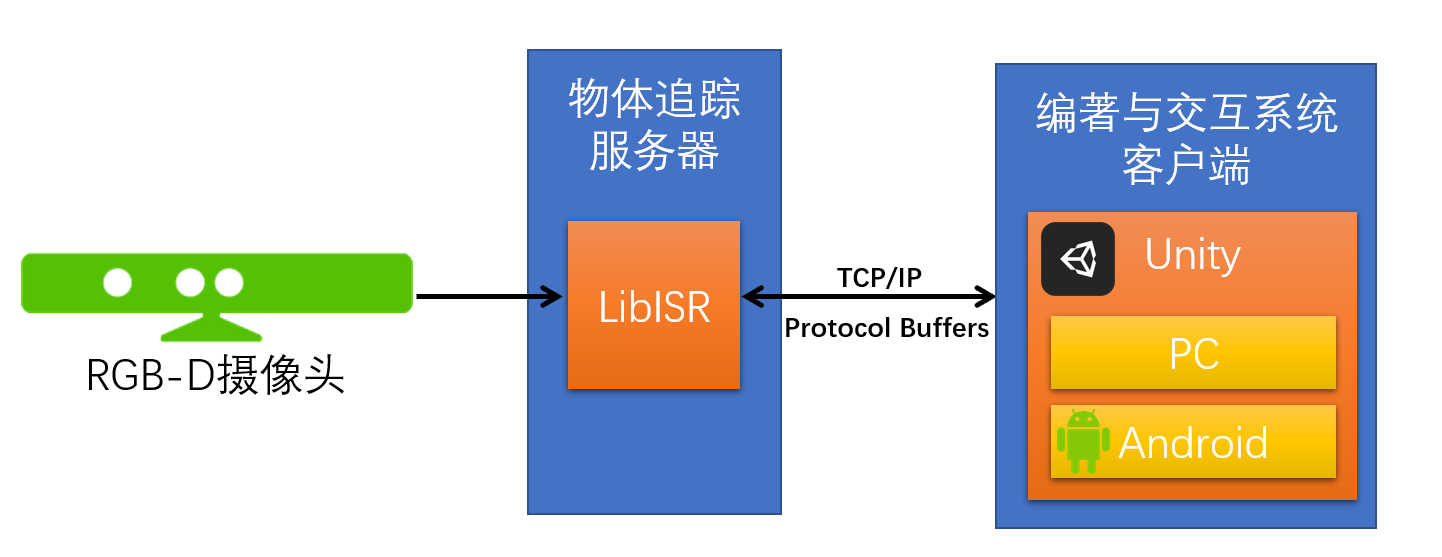
\includegraphics[width=12cm]{figure/TotalArc.png}
  \bicaption[系统架构图]
    {系统架构图}
    {The System Architecture Design}
 \label{fig:totalarc}
\end{figure}

综上所述,物体追踪引擎作为服务器,而编著和交互系统作为客户端,两者通过网络通信,本章节将会对这三部分的设计进行详细的介绍。

\section{服务器设计}

物体追踪引擎以LibISR为核心\cite{Ren_3DV_2014, star3d_iccv_2013},他的整体架构如图所示,其中只保留了比较核心以及在原程序上进行了一定修改的类。

\begin{figure}[!htp]
  \centering
  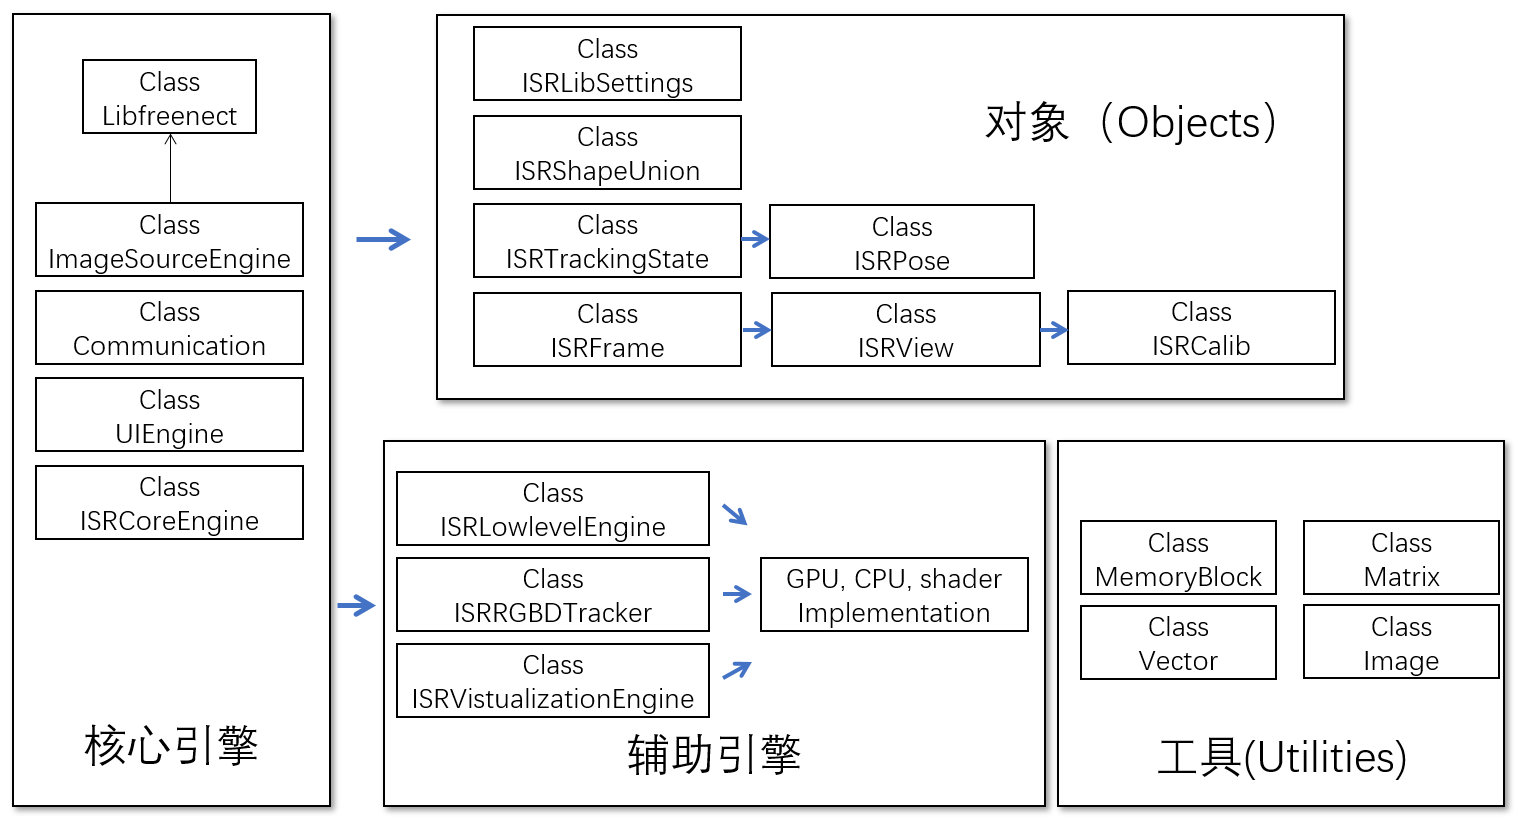
\includegraphics[width=12cm]{figure/LibArc.png}
  \bicaption[物体追踪架构图]
    {物体追踪架构图}
    {The Object Tracing Engine Architecture Design}
 \label{fig:labarc}
\end{figure}

整体架构共分为核心引擎、辅助引擎、对象、工具四部分。运行时,函数首先使用核心引擎进行初始化,包括使用的模型数据、追踪要求、标定数据等等,然后由负责网络、追踪、用户接口(UI)的引擎完成各自工作。这些工作涉及到的数据被封装为对象类。同时,LibISR还提供了一套自己的基础数据结构。

\subsection{对象}

对象是一些不包含业务逻辑,只负责将数据进行封装、整合、处理的类。首先对这些对象进行介绍,可以方便之后的讲述。

\begin{itemize}
    \item \textbf{ISRCalib}
用于储存标定数据,包括深度摄像头和彩色摄像头的内参、外参,以及单质性矩阵,这些标定数据又由单独的对象类进行储存。相机本身的参数通过读取标定数据文件进行读取,而单质性矩阵则通过计算上述变量得出。
    
    \item \textbf{ISRPose}
储存物体的追踪结果,追踪结果由物体的旋转矩阵和位移向量组合起来的4x4矩阵。
    
    \item \textbf{ISRView}
储存相机读取的图像以及经过处理的中间数据。包括原始的彩色图像、深度图像,以及将彩色图映射到深度图的图像等。

    \item \textbf{ISRFrame}
储存了RGB-D图片的中间处理结果,例如点云、碰撞图、ISRView。
    
    \item \textbf{ISRTracingState}
主要用于多物体追踪,保存所有物体的ISRPose,被用于计算代价函数。

    \item \textbf{ISRShapeUnion}
主要用于多物体追踪,保存由所有物体的模型组合而成的shape union。

    \item \textbf{ISRLibSettings}
保存项目的相关设置,包括是否使用GPU加速,是否追踪一种模型等。
\end{itemize}

\subsection{核心引擎}

核心引擎是暴露给用户的接口,负责启动物体追踪、与硬件、网络、用户交互等核心功能。用户可以通过创建核心引擎的对象,从而实现物体追踪的功能。

\begin{itemize}
    \item \textbf{ImageSourceEngine}
该类是一个纯虚类,他负责连接硬件(摄像头),将读取到的数据进行格式转换、适配,保存在ISRView中,并将指针提供给其他引擎以供图片读取。
    
    \item \textbf{Communication}
该类作为服务器,负责开启数据传输服务,等待前端用户输入并进行处理。
    
    \item \textbf{UIEngine}
该类主要负责通过OpenGL实现用户前端,将追踪的原始RGB图像、深度图像、追踪结果进行显示。并且通过glut的接口,获得用户输入,包括开始、重置、暂停、截屏等等。

    \item \textbf{ISRCoreEngine}
它是物体追踪的核心引擎。在每一帧都会运行,将获取的图片进行处理,调用ISRRGBDTracker对象进行计算,获得物体位置后更新ISRTrackingState等对象,并且调用ISRVisualisationEngine将追踪的结果使用OpenGL进行可视化,之后由UIEngine进行显示。

\end{itemize}

\subsection{辅助引擎}

辅助引擎是辅助ISRCoreEngine进行工作的类,包含部分业务逻辑。这三类都是纯虚类,会根据硬件情况采用C++代码或CUDA\cite{CUDARef}代码的实现。

\begin{itemize}
    \item \textbf{ISRLowlevelEngine}
该类负责融合RGBD图像、应用滤波、获得bounding box、根据RGBD图像获得点云数据等功能
    
    \item \textbf{ISRRGBDTracker}
用于进行物体追踪的计算,包括标记前后景像素、计算代价函数、计算Jacobian矩阵用于最小化代价函数等功能的实现。
    
    \item \textbf{ISRVisualisationEngine}
用于中间数据的可视化,以及最终结果的渲染,包括渲染被追踪的物体、渲染深度图、渲染SDF模型应用结果等。
\end{itemize}

\subsection{工具}

LibISR基于C++基本的数据结构进行了进一步的封装,实现了向量(vector)、矩阵(matrix)、图像(image)、数据块(memory block)等数据结构。向量和矩阵再提供基本运算的基础上,还提供了针对于实际需求的成员变量名字,例如Vector3具有r,g,b三个成员,或x,y,z三个成员。此外,图像还提供了保存为文件的函数。数据块则为了统一管理在CPU和GPU进行转换的数据。

\section{编著与交互系统客户端设计}
前端基于Unity引擎进行实现。应用由Game Manager进行控制,包括应用当中的各个场景。其中编著系统主要在Build Experiment场景中,而通过追踪技术与物体交互的部分则主要在Tracing Scene场景中,此外还设计了其他场景。本小节将对这些场景的设计进行介绍。

\begin{figure}[!htp]
  \centering
  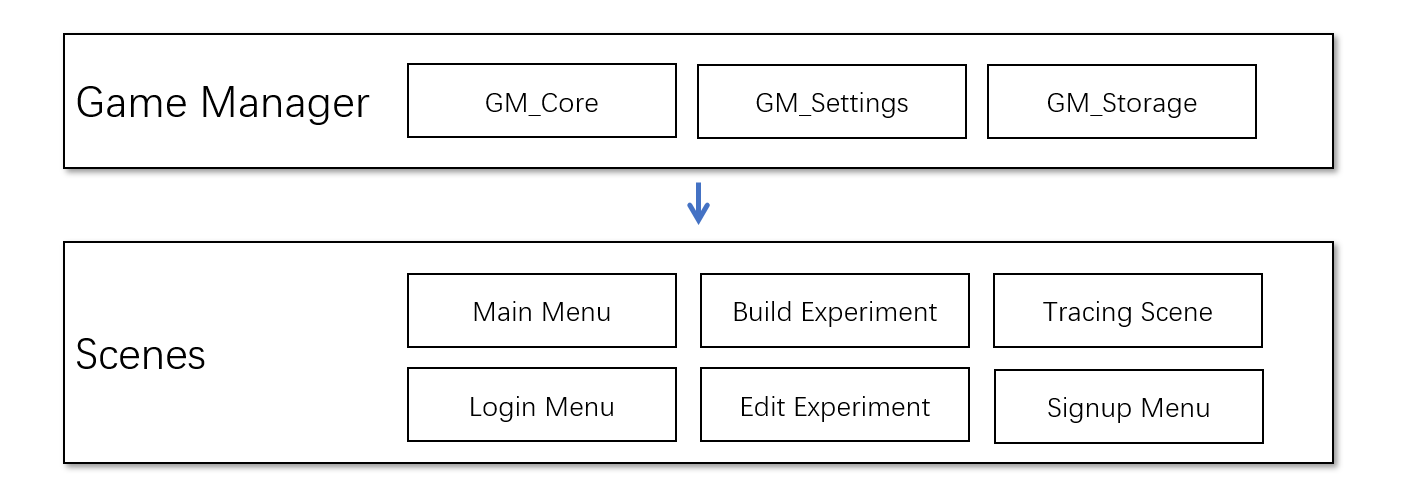
\includegraphics[width=12cm]{figure/GMarc.png}
  \bicaption[游戏管理器与场景架构设计图]
    {游戏管理器与场景架构设计图}
    {The Game Manager and Scenes Architecture Design}
 \label{fig:gm}
\end{figure}

\subsection{游戏管理器}
应用通过游戏管理器(Game Manager,GM)进行统一管理,负责的功能如下。
功能其一,它控制场景之间切换的异步加载逻辑并提供切换场景的接口,从而可以清晰、统一的管理所有场景之间的逻辑关系和跳转逻辑。其二,它保存生命周期跨场景并且由用户进行的变量,这些变量不能随着场景被切换而被销毁,也不能在应用中以静态变量的形式存在,如登陆应用的账户信息、实验编著的结果等。其三,它提供了场景中静态变量的读取接口,因为这些变量需要在多个对象中使用,而且会随着应用开发进程产生变动,因此需要统一管理,包括系统支持的事件行为、器具类型、物质等等。而这些物体的信息则是保存在GM\_Storage中的。最后,由于在一部场景加载的时候,场景的光照设置是不会被修改的,因此不同于其他场景的光照,例如天空盒,需要针对每个场景进行单独的调整。而每个场景中的光照参数就被保存在GM\_Settings中。

\subsection{编著场景}
编著场景为Build Experiment,负责创建、编辑实验场景。由游戏管理器进行管理。其中的架构分为三层。

\begin{figure}[!htp]
  \centering
  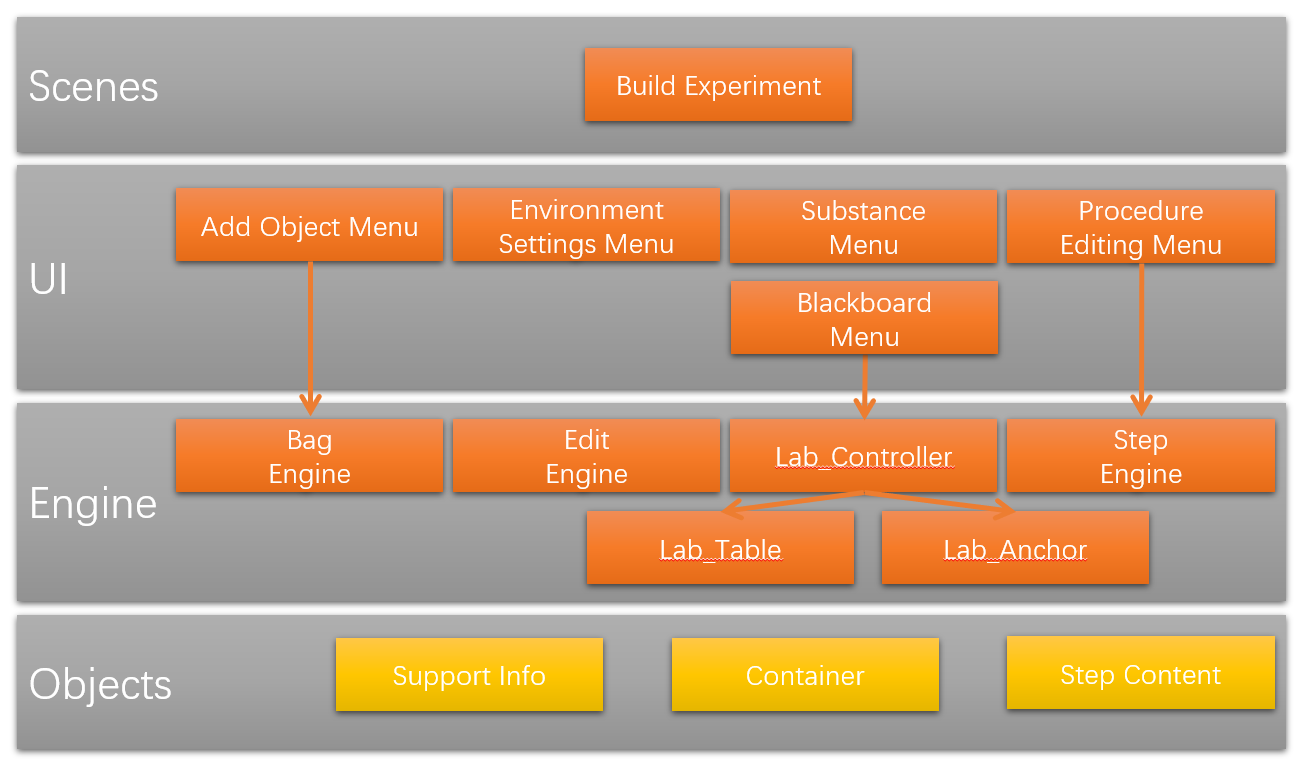
\includegraphics[width=12cm]{figure/buildearc.png}
  \bicaption[编著场景架构设计图]
    {编著场景架构设计图}
    {The Building Experiment Scene Architecture Design}
 \label{fig:gm}
\end{figure}

最上层为用户接口(User Interface,UI),他保存了用户前端的控件。前端控件除了基本的按钮之外,主要分为四块。

\begin{itemize}
    \item \textbf{Add Object Menu}
用户可以通过此菜单向场景中添加物体,在菜单中对各类物体进行分类,对于化学实验来说,包括容器、物质、器具、预置组合四类。
    
    \item \textbf{Environment Settings Menu}
用户可以通过此菜单修改实验场景,例如场景的灯光强度、颜色、室内还是室外环境、相机的高度、角度等。
    
    \item \textbf{Blackboard Menu}
用过可以通过此菜单修改实验中黑板上的实验信息的大小、颜色,包括标题和正文两个部分。

    \item \textbf{Substance Menu}
用户可以通过此菜单修改添加的物质的种类和量。

    \item \textbf{Step Menu}
用户可以通过此菜单修改实验的流程、标题等内容。
\end{itemize}
~\\
\indent    	上述的控件需要第二层,引擎进行支撑。由于编著系统很大程度上集中在UI的部分,因此引擎大部分是为UI进行服务的。除了上述的控件之外,还包括应用的交互

\begin{itemize}
    \item \textbf{Bag Engine}
用于控制Add Object Menu。其中包括Menu出现和消失的动画、菜单内部转换逻辑、获取用户希望添加何种物体,并且想更底层的引擎传递等功能。
    
    \item \textbf{Edit Engine}
用于管理编辑场景的所有数据,包括场景中添加物体的位置、种类、量,黑板文字的位置、颜色、大小,场景中的环境数据等,在编辑完成的时候将所有数据采用固定的格式进行保存,在编辑场景的时候从该数据结构中进行读取并且还原。
    
    \item \textbf{Step Engine}
用于控制Step Menu。负责用户创建、编辑每个实验对应的流程信息。

    \item \textbf{Lab Controller}
是交互的核心控制引擎,获得鼠标(或手指触摸)事件,运行相应的业务逻辑。判断输入的是点击事件还是长按时间,如果是点击事件则弹出编辑界面,包括提示信息的编辑界面(Blackboard Menu)、物质的编辑界面(Substance Menu)两种。如果是拖动事件,则将被点击的物体或文字进行移动。在编辑已有实验的时候,需要从游戏管理器中读取已创建的物质以及黑板信息数据,并且进行还原。在桌面上拖动时,可以选择固定的锚点上,或是锚点控制不到的任意位置。设置锚点的目的是可以使一些必要的仪器保持固定的相对位置和顺序,这些锚点本身是由Lab Anchor进行维护,包括为一个锚点添加、替换、删除物体。Lab Anchor由Lab Table进行统一维护,包括在删除、移动、添加物体的时候控制所有锚点的行为,例如在添加物体的时候,在制定锚点出空出位置,再删除物体的时候,由其他锚点的物体补上等。

    \item \textbf{Button}
对于场景中一直显示的按钮,如展开环境设置菜单的按钮,展开加入物体菜单的按钮等,由Button统一实现事件函数。他还控制在有面板被展开的时候暂停Lab Controller中物体控制的逻辑,避免用户在使用前端UI的时候操作干扰到实验编辑。
\end{itemize}
~\\
\indent    	上述逻辑需要使用一些持久化的对象,控制他们的变量,这些对象包括保存用户创建的物质的种类和量的对象Container,保存用户创建的步骤和流程的对象Step Content,保存实验提示信息的颜色和大小信息的text,以及保存系统支持的物质和时间类型的对象Support Info。

此外,由于创新新实验和编辑已有实验共用该场景,因此需要对场景中的编辑数据进行保存,这里使用了类Experiment Setup进行保存。其UML类图\ref{fig:uml}如图所示。


\begin{figure}[!htp]
  \centering
  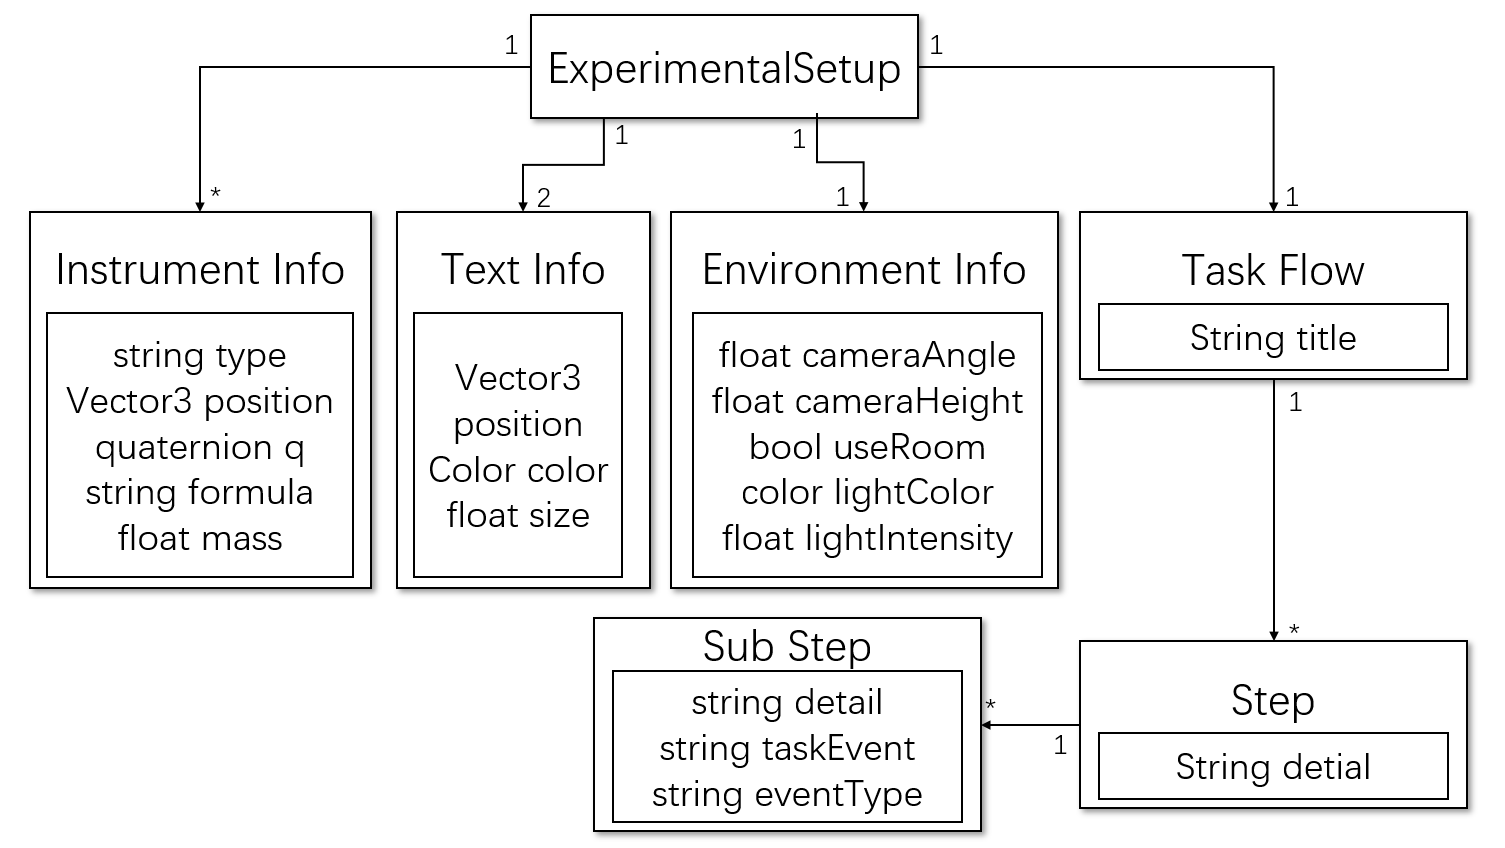
\includegraphics[width=12cm]{figure/setupclass.png}
  \bicaption[编著信息UML类图]
    {编著信息UML类图}
    {The UML's class Diagram of Authored Data}
 \label{fig:uml}
\end{figure}

其中编著信息由四部分组成。每个场景有多个instrument info保存创建的物体的位置、旋转、物体种类、其中含有的物质的名字及其物质的量。每个场景由两个text info,分别用来储存实验提示信息中的标题和正文的位置、大小、颜色信息。每个场景包括一个environment info,用来保存场景中相机、光照的相关属性。每个场景还包括一个task flow,用来保存编辑的实验流程。每个实验流程有多个流程(step),每个流程又有多个步骤(substep),步骤中包含步骤名称、对应的事件等信息。

\subsection{交互场景}
交互场景用于将用户创建的物体根据物体追踪的结果渲染到增强现实场景中。

\begin{figure}[!htp]
  \centering
  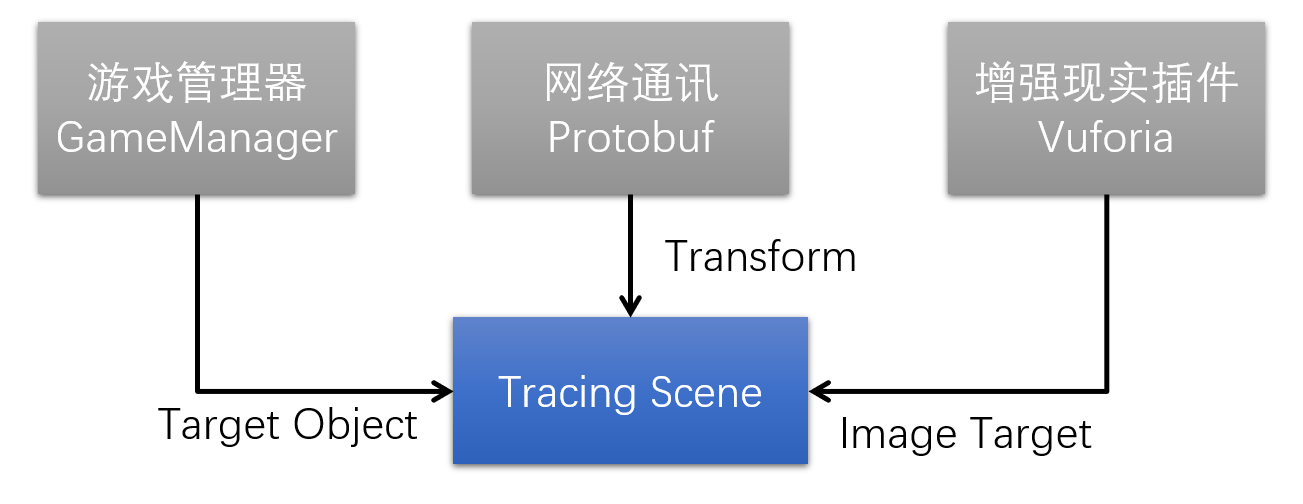
\includegraphics[width=12cm]{figure/tracingScene.png}
  \bicaption[交互场景架构设计图]
    {交互场景架构设计图}
    {The Interaction Scene Architecture Design}
 \label{fig:int}
\end{figure}

场景主要由三个组件构成,首先场景会通过游戏管理器获得要用于显示的被追踪物体的相关数据。然后根据Vuforia识别出场景中的标志物,他相对于真实场景静止,用于为Unity确定真实场景的位置和坐标系。之后会打开网络通讯,将追踪结果应用到应被渲染的物体上,就可以实现虚实融合了。


\subsection{其他场景}
除上述场景之外,系统还实现了主页、登录页面、注册页面等场景。它们结构与上述框架类似,而且比较简单。

主页主要负责场景之间的跳转,提供三个按钮,用户用户进入编辑场景、编辑已有场景、进入交互场景。交互逻辑仍然由游戏控制器负责。

登陆和注册页面前端进行用户输入,然后通过引擎发送网络数据到服务器进行输入检查,如果出现错误则进行错误提示,输入正确的逻辑仍然由游戏控制器负责。

\section{网络通信设计}
\begin{figure}[!htp]
  \centering
  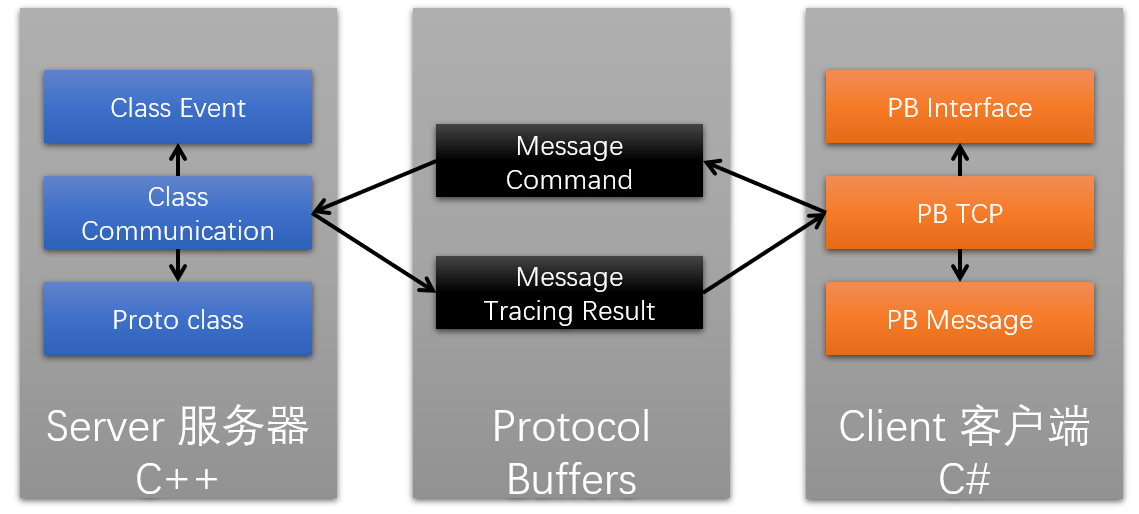
\includegraphics[width=12cm]{figure/netarc.png}
  \bicaption[网络通信架构设计图]
    {网络通信架构设计图}
    {The Network Communication Design Architecture}
 \label{fig:gm}
\end{figure}
应用需要在C++实现的服务器和C\#实现的客户端之间进行通信。通信采用了共同的关键字(Message),即command和tracing result。

Command储存的是客户端向服务器发出的指令,包括指令种类,如启动程序录制、启动物体追踪、结束程序等。还包括指令所需要的变量,如追踪物体的种类等。Tracing Result为服务器向客户端返回的追踪结果,是一个由ISRPose的旋转、位移矩阵构成的数组。关键字分别在两端以各自形式的类存在。

在共同的关键字的基础上,两端都实现了各自的socket。服务器在communication类中建立服务,客户端在PB\_TCP中发送请求。服务器获取到客户端请求后通过触发事件运行响应函数。客户端通过PB\_Interface调用相应的函数。

	 \chapter{系统实现}
\label{implement}

本章节将对于上述设计的实现过程进行叙述。本章节分为三部分。第一部将介绍本系统如何基于LibISR的物体追踪系统\cite{Ren_3DV_2014, star3d_iccv_2013}实现后端服务器。第二部分将介绍本系统如何基于Unity引擎实现编著和交互系统,包括应用的游戏管理器的实现,以及应用中各个场景的具体实现。其中重点介绍编著系统对于用户需求中的各个功能的实现,以及交互场景中将服务器的物体追踪数据应用到最终的增强现实场景中的物体上的实现方法。第三部分将介绍在客户端和服务器之间进行通讯的实现。

\section{物体追踪系统的实现}
本系统基于开源物体追踪工具,LIbISR进行实现。在使用原有算法的基础上,进行了一定的修改。本系统使用的深度摄像头是Kinect第二代,但是原工具是基于第一代开发的。两代摄像头存在着一定的差异,包括驱动的支持情况、图像的分辨率等。这些因素导致了源程序并不能直接运行,本系统在开发过程中对其进行了一定的修改。

\subsection{Libfreenect 2的适配}

原系统使用openni为驱动获取Kinect数据。但是openni并不能有效获取Kinect 2的数据,并且已经停止更新和维护了。因此本系统使用了Libfreenect 2作为替代。

LibISR对于不同的硬件提供了统一的接口ImageSourceEngine。它是一个纯虚类,只需要添加新的实现,并且在初始化的时候进行修改就可以使用不同的驱动了。在实现时,保存了Private data类,将驱动的不变数据,例如device指针,listener指针,以及从相机获取的数据进行保存。实现获取图像,需要首先根据文档要求进行初始化。初始化时,软件遍历连接的USB接口获取设备,选择使用CUDA进行加速,初始化RGB、红外线发生器、深度摄像头三个设备,配置深度摄像头的范围。Libfreenct 2还自带了使用Kinect默认标定数据生成RGB-D图像的功能,经过验证也具有比较好的融合效果,但是本系统仍然使用了自己的标定数据,Libfreenect 2只提供了融合之后的图片,而缺乏中间数据。此外,Libfreenect在初始化之后没有被使用的话就会被自动关闭,但是LibISR需要在初始化图像源之后进行其他操作,因此这里创建了新的线程,在初始化之后就会进入死循环,在软件结束之后回收,保证驱动不会自动关闭。

初始化之后,程序每一帧会调用该函数获取图像。获取图像时会首先获得数据在CPU当中的指针,然后将获取到的图像进行逐一复制。LibISR中图像都是基于数组封装的,但是进行逐一复制而不是memory set的原因是,RGB图像摄像头获得的数据是BGR因此需要转换颜色通道,而深度图像摄像头获得的是32位float,而程序中实际使用的是16位short int。

转换完成后,就可以将获取的图像应用到后面的计算了。

\subsection{相机标定与RGB-D图像融合}
由于Kinect 1的彩色图像分辨率为640*480,深度图像分辨率为320*240,两者成比例,并且可以通过设置驱动直接获得相同分辨率的图片,因此源程序存在应用错误、逻辑基于两者分辨率相同的情况。但是,Kinect 2的彩色图像分辨率为1920*1080,深度图像分辨率为512*424,不成比例。因此需要在获得图像后进行融合。为了融合两个相机的图像,需要找到深度图中每个像素点对应在RGB图像中的坐标。

这一过程需要对相机标定从而获得相机参数。本项目的标定使用了基于ROS系统的iai kinect提供的标定工具\cite{iai_kinect2}。该系统通过拍摄多个角度的确定规格的棋盘格,可以计算出RGB相机和深度相机的内参,包括相机的焦距以及图像中心等。同时,通过在同一时刻获得相机的深度图像和RGB图像,可以获得相机的外参,即深度摄像机和RGB摄像机之前的位移和旋转关系。之后可以通过他们计算出坐标映射公式。

设$P_{rgb}$,$P_{ir}$分别为彩色摄像头和深度摄像头各自的相机坐标系下的一点的非齐次坐标,对应的像平面坐标分别为$p_{rgb}$,$p_{ir}$,彩色摄像头和深度摄像头的内参矩阵为分别为$H_{rgb}$和$H_{ir}$,根据相机的映射公式,可得相机坐标系与像平面的点的对应映射关系为:
\begin{equation}
 p_{ir} = H_{ir}P_{ir} \quad\mathrm{,}\quad  p_{rgb} = H_{rgb}P_{rgb}\label{camera1}
\end{equation}
由标定可以得到两个摄像机之间的外参矩阵,包括旋转矩阵R和平移向量T。则两者相机坐标系之间的对应关系为:
应映射关系为:
\begin{equation}
 P_{rgb} = RP_{ir} + T \label{camera2}
\end{equation}
将公式(\ref{camera1}),(\ref{camera2})整合,可以得到两个相机的像平面之间的点的映射关系为:
\begin{equation}
 p_{rgb} = H_{rgb}RH_{ir}^{-1}p_{ir} + H_{rgb}T
\end{equation}
由此公式就可以得到深度图像中每个点在彩色图像中的点的坐标了。为表达简便可设置
\begin{equation}
 H = H_{rgb}RH_{ir}^{-1} \quad\mathrm{,}\quad T_H = H_{rgb}T
\end{equation}

由$H$,$T_H$构成的矩阵就是单应性矩阵了,它描述的是彩色相机和深度相机的像平面之间的映射关系。由于其中的像平面坐标为三维非齐次坐标,但实际使用的时候为二维坐标,也就是三位齐次坐标,因此需要在使用时进行转换,其中三维非齐次深度坐标的z值就是该点的深度。
	
本系统在Low Level Engine中实现了融合。为了运算效率考虑,系统中将深度图映射到了彩色图,使用深度图的分辨率。融合使用了CUDA代码,首先将数据从CPU复制到GPU,并且分配所需要的线程块和线程数目。在本系统中,使用了8*8的线程块(block)结构,以及64*53的网格结构,从而实现将每个像素分配到一个线程。由于CUDA代码中每个线程运行的时候都可以获得自己的block ID和thread ID,再加上block的结构,就很方便的计算出对应的像素位置。得到像素的位置,就可以利用上述的单应性矩阵公式计算出该像素在彩色图中对应的位置了。
	
\begin{equation}
 X_{rgb} = threadID.x + blockID.x * blockDims.x
\end{equation}
\begin{equation}
 Y_{rgb} = threadID.y + blockID.y * blockDims.y
\end{equation}

这一部分函数输出了两张图,一张是融合之后的RGB-D图,其中a通道代表深度值。另一张是对齐的彩色图,它是将RGB-D图像的a通道设为1之后得到的,彩色图缩小之后可以与深度图对齐的图像。

\subsection{追踪结果显示}

由于Kinect 1中两幅图成比例,因此UIEngine可以在基于深度图大小计算出追踪结果后将其按比例放大叠加在彩色图上。但是,当二者不成比例时,追踪结果就会出现扭曲。因此这里使用了对齐之后的rgb图像作为代替。虽然这样做不会有实质的影响,但是由于对齐之后的彩色图存在硬件造成的噪声和重影,会对显示效果有一定的影响。

\section{客户端的实现}
本小节将详细介绍按照设计的架构,包括绍游戏管理器,以及应用中各场景的实现。

\subsection{游戏管理器}
游戏管理器会在基准场景(base scene)中生成,而且这个场景不会被销毁。为了保证只有一个游戏管理器,在初始化的时候使用了单例模式,GM\_Core中包含了一个静态指针,指向一各游戏管理器实例。当其他对象尝试创建新的对象的时候,会被销毁。

在每次需要切换场景的时候,游戏管理器会先将当前场景(如果有的话)进行卸载,然后启动coroutine异步加载另一个场景,该场景的加载模式为additive,表示在当前场景的基础上进行加载。加载完成之后该coroutine会进行返回,返回之后会根据新的场景中GM Settings的情况修改场景光照。如果加载过程太长的话,在这一个过程中可以添加等待场景加载的动画。

\subsection{编著场景}
编著功能主要在Build Experiment场景中进行实现,本小节将首先介绍场景中的用户接口(UI),然后根据实现需求进行相应的介绍。

\subsubsection{用户接口(UI)实现}
编著场景中实现了五个用于交互的菜单。

\begin{itemize}
    \item \textbf{Settings Menu}
用于修改实验场景。实验环境编辑需要调整光照颜色与强度,相机高度与角度,实验环境(室内或是室外)等。因此使用了滑块(Slider)和开关(Switch)等控件,并添加一个半透明panel用于和场景区分。滑块封装了OnValueChange函数,会在滑块发生移动的时候触发。相似的,开关控件会在被修改的时候调用控制函数。
    
    \item \textbf{Tool Menu}
用于添加物体。用户点击添加物体按钮后,会播放动画将选择物体类别的菜单显示出来,用户可以选择要添加的物体类别,之后软件显示所有支持物体的图片,点击对应图片就可以添加物体了。选择物体类别的菜单由UI\_List实现,目前支持“容器”、“药品”、“工具”、“预置组合”四类。UI\_List本身具备垂直布局(vertical layout),它会将子对象自动按照竖直排列。而每一个子对象对应一种物体类别,并且绑定了onclick函数。选择类别后弹出的选择具体物体的菜单由UI\_Bag实现,他也包含了一个网格布局(grid layout),会自动将子对象按照网格排列。他的子对象都是预制体(prefab),可以显示图片,并且绑定了创建物体的onclick函数。
    
    \item \textbf{Substance Menu}
用于编辑药品属性和量。其中包括,选择物质种类的下拉框(dropdown),以及输入物质的量的输入框(input field)。下拉框使用了OnValueChange函数,在选择发生变化的时候触发。输入框绑定了OnEndEdit,在编辑完成的时候触发。

    \item \textbf{Blackboard Menu}
用于编辑场景中的实验提醒文字。包括调整文字的大小和颜色,设置与settings menu类似。
    
    \item \textbf{Step Menu}
用于设置实验的步骤等信息。最上方设置了输入实验名称的输入框。一侧使用了vertical layout显示当前的已有的流程,另一侧显示当前已有的步骤。这里的流程和步骤都使用了同一个预置体。中间提供了输入流程名称、步骤名称的输入框,以及选择对应事件的下拉框。他们都绑定了对应的OnValueChange函数,在获得用户输入的时候触发。
\end{itemize}
~\\
\indent    	这些菜单会通过场景中的按钮或用户输入触发,同时会暂停触发场景其他交互行为,防止在用户调整菜单的时候出现干扰。在菜单之下还会生成一个覆盖整个屏幕的透明按钮,实现当用户点击的时候关闭菜单,并且确定用户输入输入,恢复场景其他交互。

\subsubsection{实验场景编辑}
当用户点击场景编辑按钮后,会弹出编辑场景的菜单(Settings Menu)。当用户移动其中的滑块时,会触发OnValueChange函数,调用控制Slider的引擎,UI\_Slider,它保存了场景中相机、光源的指针,会读取此时slider的值,并且修改对应物体的属性值。如果通过开关调整实验环境,开关的控制器会修改对应的场景模型。

\begin{figure}[!htp]
  \centering
  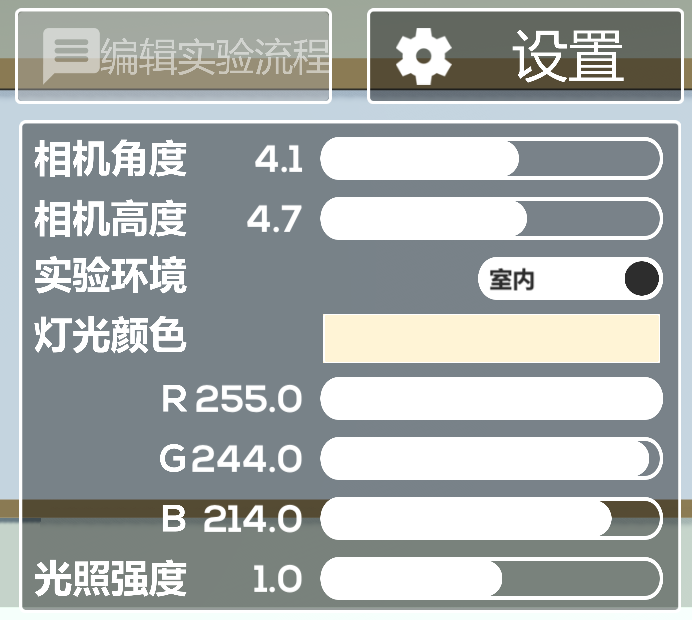
\includegraphics[width=8cm]{figure/settings.png}
  \bicaption[实验场景编辑用户接口截图]
    {实验场景编辑用户接口截图}
    {The Screenshot of Experiment Editing UI}
 \label{fig:gm}
\end{figure}

\subsubsection{物体编辑}
场景中的物体首先通过菜单进行添加。支持物体以及他们的种类通过静态二维链表储存。

	当用户选择添加物体之后,选择物体种类的菜单弹出(Tool Menu)。物体种类被选择后,控制器UI\_List会查找二维链表,获得对应类别的物体图片,并创建显示该图片的预制体,添加到选择物体的菜单中。用户选择物体之后,会通过对应物体的名字,在资源文件夹中查找对应的预制体游戏对象,添加到场景中,完成物体创建。
	
\begin{figure}[!htp]
  \centering
  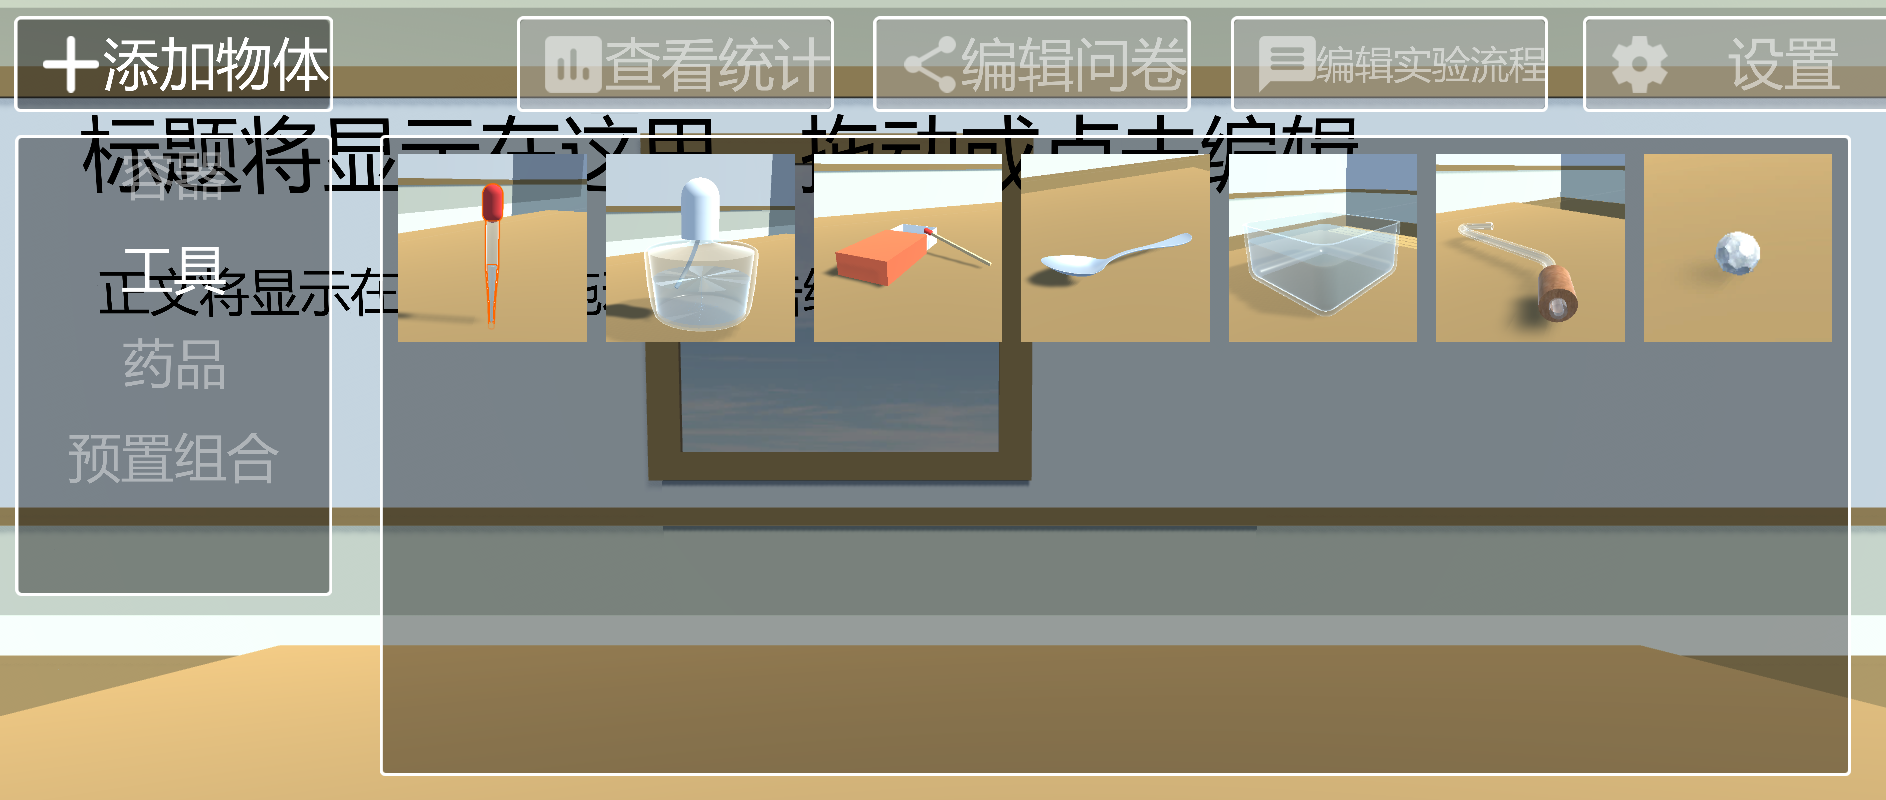
\includegraphics[width=12cm]{figure/addObj.png}
  \bicaption[添加物体用户接口截图]
    {添加物体用户接口截图}
    {The Screenshot of Adding Object UI}
 \label{fig:gm}
\end{figure}

	创建好的物体通过控制器Lab\_Controller进行控制。Lab\_Controller会在用户触发点击事件的时候,从相机位置向点击位置发出一条射线,之后获取射线碰撞的第一个物体。同时,控制器会在每一帧计算距离用户点击时刻的时长,如果在到达一定的阈值之前检测用户松开鼠标,则触发单击对应的事件。如果超时,则会判断用户触发拖动事件。

	如果是单击事件,首先判断接触到的是否是可以编辑的物质,判断的方式是该物体是否具有container类,该类用于保存物体包含的物质的种类和量。如果有,则将编辑物质的菜单(Substance Menu)进行显示。下拉框会在初始化的时候获取所支持的物质,并且修改选项。为了保证物质的量为浮点数,需要对输入框的格式进行设置。完成编辑后,控制器会将对应的用户输入赋值到该物体的container对象中。如果没有,则无效果。
	
\begin{figure}[!htp]
  \centering
  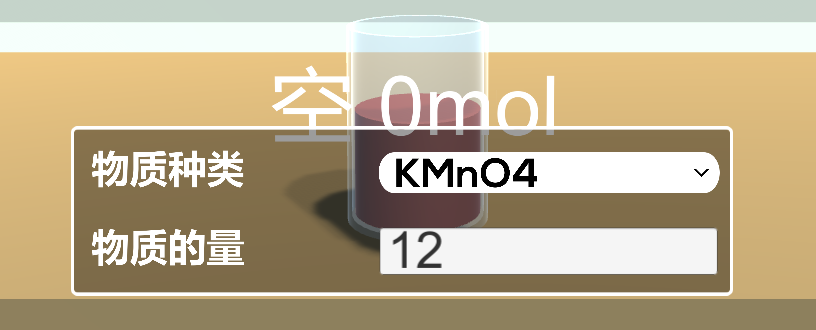
\includegraphics[width=12cm]{figure/subs.png}
  \bicaption[编辑物体种类用户接口截图]
    {编辑物体种类用户接口截图}
    {The Screenshot of Editing Object UI}
 \label{fig:subs}
\end{figure}

编辑好的物体会将物质信息显示在模型外,效果见图\ref{fig:subs}和\ref{fig:substi}。显示的文字通过3D Text实现,会在修改之后触发相应的函数修改其text mesh的内容。

如果是拖动事件,依然首先判断物体是否是可以移动的物体,所有添加的物体都是可以移动的,他们使用Object的标签进行标记。这里的目的是避免拖动桌子、墙壁等其他静态物体。之后会在每一帧由相机向点击位置发出射线,将当前拖动的物体放置在射线和碰撞体的交点上。此时需要先去除拖动物体的碰撞体,否则物体会沿着射线方向一直向相机移动。当用户松手的时候,物体就会停留在最后移动的位置,并且恢复物体的碰撞体保证可以进行下一次移动。

由于一些实验中往往需要流程化的实验步骤,例如产生气体之后通入水槽等,需要气体发生装置和收集装置相对位置固定,因此添加了UI\_Anchor进行引导。UI\_Anchor是与桌面平行的平面碰撞体,当上述的交点接触到锚点(anchor)时(同样使用tag进行标记),会在锚点中心生成一个目前拖动物体的复制,并且修改它的材质为半透明单色,并把该物体的指针赋给UI\_Anchor中的对应变量。如果此时用户松开鼠标,则拖动中的物体就会代替复制,被固定在锚点上。当用户需要将物体从锚点移开的时候,则会制造先出复制,直到点击位置离开锚点范围之后删除复制,在这过程中如果用户松开鼠标,则物体会返回锚点处。。
	
\begin{figure}[!htp]
  \centering
  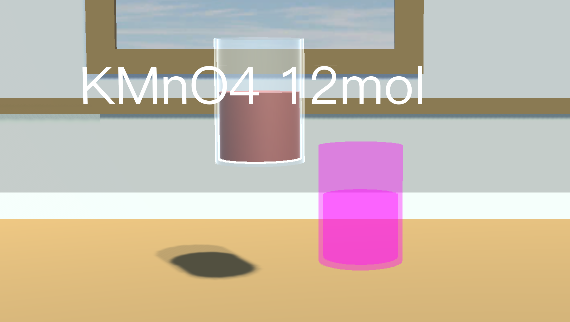
\includegraphics[width=8cm]{figure/substi.png}
  \bicaption[锚点物体复制效果图]
    {锚点物体复制效果图}
    {The Effects of Objects Substitution on Anchor}
 \label{fig:substi}
\end{figure}

场景中有多个平行锚点,它们都在同一个实验桌上,由UI\_Table控制。UI\_Table会储存桌子上的锚点的物体信息,并且在鼠标移入、移出锚点,即真正添加和删除物体的时候,根据所有锚点的位置和占用情况,对其余物体进行移动操作。如果在添加的时候发现所有的锚点都被占用,则不会创建新的复制,物体也不能被移入锚点。

基于上述机制,物体在创建的时候会优先创建在锚点上。只有当物体太多、锚点都被占用的时候,才会被创建在桌面上的其他位置。综上所述,物体的创建、移动、内容编辑就实现了。


\subsubsection{提示信息编辑}
实验过程中需要显示实验名称,并且对用户进行实验步骤提示,用户可以通过编著系统修改该提示信息的位置、大小、颜色等属性。

\begin{figure}[!htp]
  \centering
  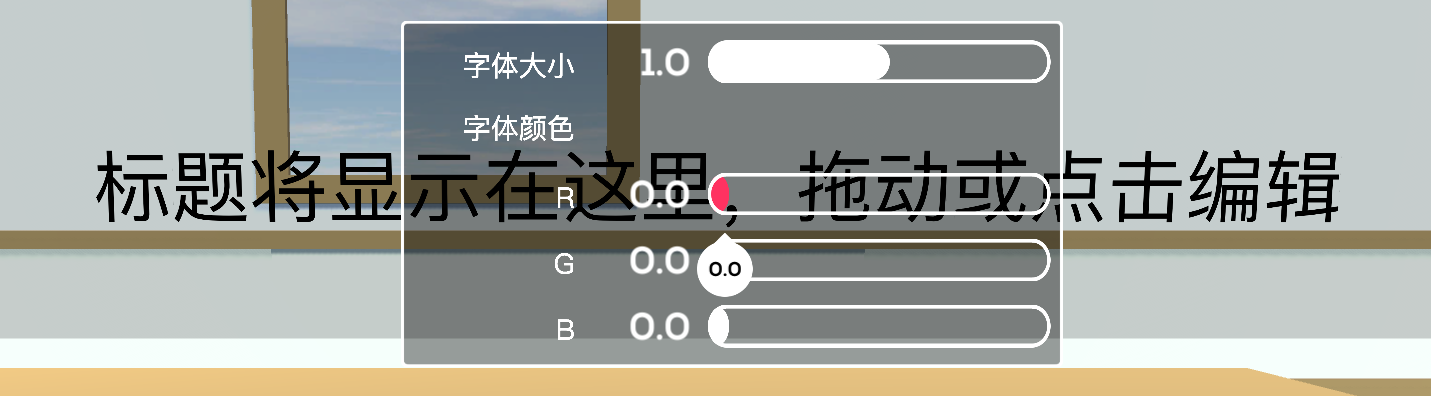
\includegraphics[width=12cm]{figure/text.png}
  \bicaption[编辑提示文字外观用户接口截图]
    {编辑提示文字外观用户接口截图}
    {The Screenshot of Editing Hints Appearance  UI}
 \label{fig:gm}
\end{figure}

用户可以编辑提示文字的显示方式。在lab controller获取到点击事件之后,如果点击的物体标签为text,则会首先获得物体中的text对象,用其中的属性值,包括字体的颜色、大小,初始化字体编辑的页面的控件的值,然后显示该菜单。用户在编辑之后,相应的文字就会被修改并立即显示了,编辑完成后,还会修改字体的text对象内的变量值,保证下一次操作的正确性。。

当用户触发长按事件,则按照与移动物体相似的逻辑移动字体,只不过在移动物体的时候如果点击位置不在字体可显示范围之内,文字就不会再发生移动。由于这些文字需要在三维场景中移动,因此也使用了3D Text。但是3D Text默认情况下会永远显示在最前面,如果需要其具有深度关系,需要修改使用的着色器。起初,系统自定义了新的着色器,但是,修改之后的着色器只能通过修改材质中的颜色参数才能修改颜色,修改text mesh的颜色是无效的,这在一些使用场景下(如WebGL)下是不被支持的。此外,需要的着色器会使文字在一定位置显示特殊的反射。最简单有效的方法,是将3D text的着色器修改为一般的2D字体的着色器,然后使用中文字体。

\subsubsection{实验流程编辑}
用户也可以通过编著系统,编辑用户在进行实验时参考的提示信息内容。

\begin{figure}[!htp]
  \centering
  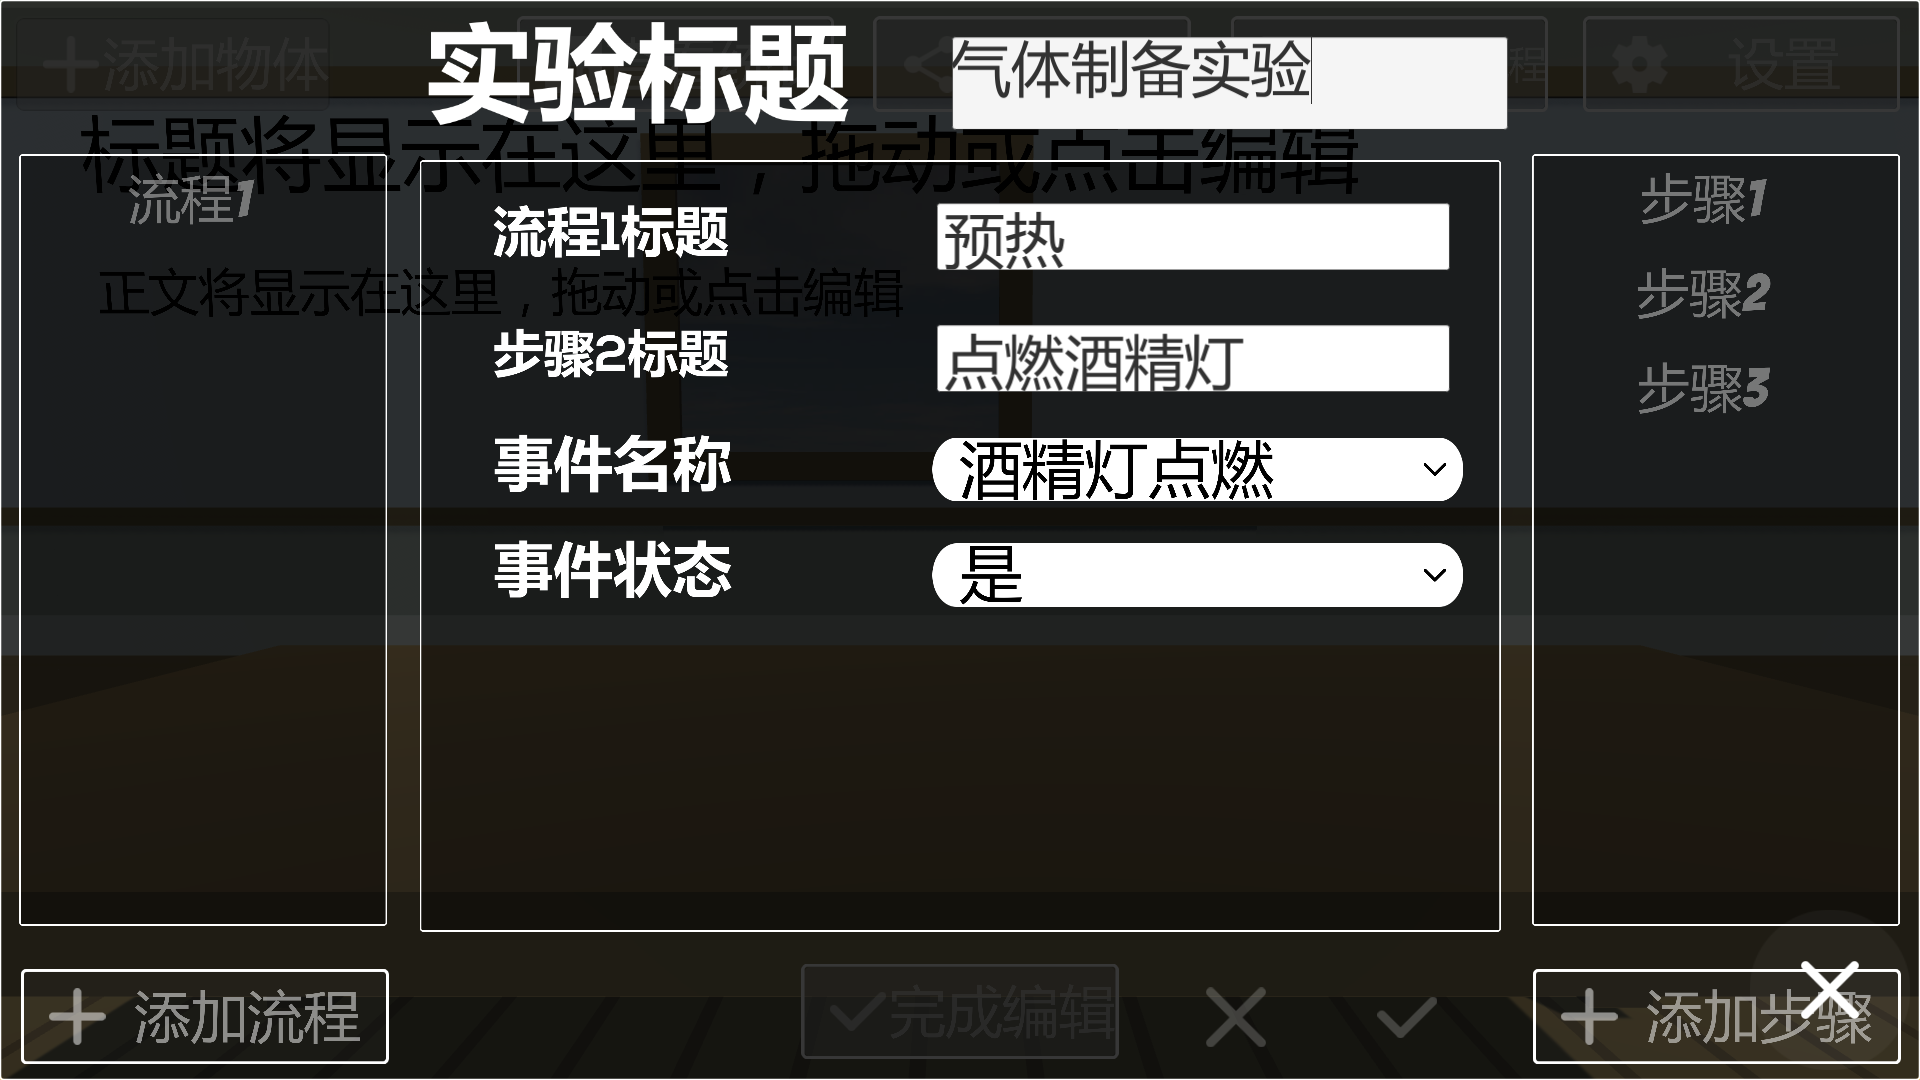
\includegraphics[width=12cm]{figure/step.png}
  \bicaption[编辑实验流程用户接口截图]
    {编辑实验流程用户接口截图}
    {The Screenshot of Editing Experiment Procedure UI}
 \label{fig:gm}
\end{figure}

当用户选择实验流程编辑的时候,会显示对应的菜单。用户首先可以添加流程,流程由预制体构成,添加的流程将会追加在显示流程的滑动框(scroll content)的子对象中,并且自动按照vertical layout进行排列。点击一个创建的流程之后可以为它添加对应的步骤,步骤使用同样的预制体实现,并使用布尔值进行区分。添加的步骤会追加在显示步骤的滑动框的子对象中。流程、步骤都可以通过输入框修改名称,步骤还需要设置对应的操作事件,可用的操作事件会在初始化的时候向游戏管理器发出请求获取,并且通过下拉框供用户选择。关于步骤、流程的上述属性都会在发生修改之后,保存在各自的step对象中。

实现过程中发现,文字输入框会产生一些中文文字不能输入的情况,这是由旧版Unity产生的bug,需要更新Unity版本进行解决。

编辑信息由UI\_Step进行控制。他保存了一个记录所有流程的指针数组,以及记录每个流程对应步骤的二维指针数组。UI\_Step还记录了当前的流程和步骤序号,当用户切换步骤的时候,会读取当前的step中的信息,并且把对应数据显示在控件上。当用户切换流程的时候,会从二维指针数组中激活对应的步骤,而将当前显示的步骤隐去。


\subsubsection{编辑已有实验}
用户可以将已经编辑的实验进行保存,并且在下一次使用的时候继续编辑。

用户需要首先将当前的编辑内容全部保存下来。负责该功能的是UI\_Edit。他会在用户保存编辑内容的时候,将场景数据保存在游戏管理器的experiment setup对象中,其结构见图\ref{fig:uml},并且通过网络发送数据,保存在数据库。其中场景的编辑数据通过编辑菜单获得,场景中的提示信息属性通过场景中的两个文字对象的相关属性获得。所有的物体创建后都会成为object list的子对象,遍历object list可以获得所有创建物体的相关属性。而实验流程则通过保存在UI\_Step中的两个列表获得。

将上述变量保存之后,在编辑已有场景的时候,场景会在初始化的时候从游戏管理器读取该对象,将所有属性还原。其中场景的还原,包括将还原的数据作用于场景中的对象上,并且修改场景编辑菜单控件的初始值。提示文字按照数据修改相应的颜色、位置等数值。物体的还原需要按照物体的名字、物质的量等信息,重新初始化游戏对象,仍然添加在object list下。步骤的还原需要按照数据,还原出所有的流程、步骤按键,并且放置在对应的滑动框的子对象下,还需要还原UI\_Step中的记录所有流程的指针数组,和记录每个流程下的步骤的二维指针数组。之后场景的还原就完成了,用户可以在此基础上继续编辑实验。

\subsection{交互场景}
交互场景中主要实现了利用追踪数据还原在Unity中的物体的姿态信息、使用Vuforia实现二维码识别,将虚拟物体与手机画面中的真实物体融合三部分。

\subsubsection{追踪结果还原}

交互场景中,需要将物体追踪服务器计算出的物体姿态进行还原。物体的姿态用一个由旋转矩阵和位移向量构成的4x4矩阵表示,其中的旋转矩阵位于矩阵左上角,可表示为
\begin{equation} 
R = 
 \begin{Bmatrix}
   m00 & m01 & m02 \\
   m10 & m11 & m12 \\
   m20 & m21 & m22  
  \end{Bmatrix}
\end{equation} 
  其中的T可以直接对应Unity场景中的位置。但是旋转矩阵则需要通过计算转换为Unity中表示旋转的四元数格式。旋转矩阵描述的是,一个向量绕单位轴$N(n_x, n_y, n_z)$旋转$\alpha$的旋转变换。公式表示为
  \begin{equation}\label{R1}
 R = 
  \begin{Bmatrix}
   n_x^2(1-cos\alpha)+cos\alpha & n_x n_y(1-cos\alpha) - n_zsin\alpha & n_x n_z(1-cos\alpha) + n_ysin\alpha \\
   n_x n_y(1-cos\alpha) + n_zsin\alpha & n_y^2(1-cos\alpha) + cos\alpha & n_y n_z(1-cos\alpha) - n_xsin\alpha \\
   n_x n_z(1-cos\alpha) - n_ysin\alpha & n_y n_z(1-cos\alpha) + n_xsin\alpha & n_z^2(1-cos\alpha) + cos\alpha 
  \end{Bmatrix}
\end{equation}
而同样的旋转可以用四元数进行表示,即
  \begin{equation}\label{R2}
Q(w, x, y, z) = [cos(\alpha/2), (sin(\alpha/2)n_x, sin(\alpha/2)n_y, sin(\alpha/2)n_z]
\end{equation}
将公式(\ref{R2})通过三角倍角公式带入公式(\ref{R1})可得
  \begin{equation}\label{R3}
 R = 
  \begin{Bmatrix}
   1-2y^2-2z^2 & 2xy-2zw & 2xz+2yw \\
   2xy+2zw & 1-2x^2-2z^2 & 2yz - 2xw \\
   2xz - 2yw & 2yz + 2xw & 1-2x^2-2y^2
  \end{Bmatrix}
\end{equation}
将公式(\ref{R3})的对角线进行加减运算,可以得到四个等式
\begin{equation}\label{R4}
\left\{
\begin{aligned}
m00 + m11 + m22 &=& 4w^2 - 1 \\
m00 - m11 - m22 &=& 4x^2 - 1 \\
-m00 + m11 - m22 &=& 4y^2 - 1 \\
-m00 - m11 + m22 &=& 4z^2 - 1 
\end{aligned}
\right.
\end{equation}
此外,还可以得到
\begin{equation}\label{R5}
\left\{
\begin{aligned}
m01 + m10 &=& 4xy  \quad\mathrm{,}\quad m01 - m10 &=& 4wz \\
m20 + m02 &=& 4xz  \quad\mathrm{,}\quad m20 - m02 &=& 4wy \\
m12 + m21 &=& 4yz  \quad\mathrm{,}\quad m12 - m21 &=& 4wx 
\end{aligned}
\right.
\end{equation}
由于四元数整体的正负是没有区别的,因此解公式(\ref{R4})取正值,带入公式(\ref{R5})可得四组解
\begin{equation}\label{R6}
\left\{
\begin{aligned}
w=\frac{\sqrt{m00 + m11 + m22 + 1}}{2} \quad\mathrm{,}\quad x = \frac{m12 - m21}{4w} \quad\mathrm{,}\quad y = \frac{m20 - m02}{4w} \quad\mathrm{,}\quad z = \frac{m01 - m10}{4w}\\
x=\frac{\sqrt{m00 - m11 - m22 + 1}}{2} \quad\mathrm{,}\quad w = \frac{m12 - m21}{4x} \quad\mathrm{,}\quad y = \frac{m01 + m10}{4x} \quad\mathrm{,}\quad z = \frac{m20 + m02}{4x}\\
y=\frac{\sqrt{-m00 + m11 - m22 + 1}}{2} \quad\mathrm{,}\quad w = \frac{m20 - m02}{4y} \quad\mathrm{,}\quad x = \frac{m01 + m10}{4y} \quad\mathrm{,}\quad z = \frac{m12 + m21}{4y}\\
z=\frac{\sqrt{-m00 - m11 + m22 + 1}}{2} \quad\mathrm{,}\quad w = \frac{m01 - m10}{4z} \quad\mathrm{,}\quad x = \frac{m20 + m02}{4z} \quad\mathrm{,}\quad y = \frac{m12 + m21}{4z}
\end{aligned}
\right.
\end{equation}
这四组解每一组的第一个值都可以作为最终结果的w值。但是,由于w太小的时候做分母会产生姿态不稳定的情况\cite{akenine2018real},因此这里实现的时候选择了四组解中w最大的一组,作为最终解。利用上述得到的四元数,可以直接在Unity引擎中应用到物体的旋转上,再将矩阵中的位移参数应用到物体的位置数据上,就可以实现将传入的矩阵应用到虚拟场景中的物体了。

\subsubsection{二维码识别}
在相关技术中提到,二维码具有对比度高、重复率低的特点,适合作为平面图片识别。

识别需要首先获得Vuforia的许可,然后将使用的图片上传到数据库,下载生成的unity package,导入到Unity场景中,并且在场景中配置权限识别码,以及匹配追踪的数据库和对应图片。然后将image target对象添加到场景中,就可以实现二维码的识别了。

设置标志的时候需要获得图片的真实大小。这里需要将图片打印出来之后测量真实长度。但是,当图片太小的时候会发生识别效果差的情况,因此需要使用比较大的二维码。

\subsubsection{虚实融合}
Vuforia识别结果会应用在场景中的image target对象中,所有需要在增强现实场景中显示的物体都需要在它的子对象中。由于物体在初始的追踪场景中与水平面就存在90度的倾角,因此在Unity场景中的物体初始化与水平面平行,倾角为0,这样才能保证二者在运行后保持相对一致。因为需要永久保持这90度的差距,因此将该物体Object设置为Image Target的一个空子对象Empty Target的子对象,并且与该对象保持90度夹角。

物体追踪的结果会应用在Empty Target上。这里需要将物体在LibISR的物体坐标系下的物体,转到Unity场景中的坐标系,再转到识别图片image target的坐标系下。保持二维码在真实场景中固定可以使得二维码的坐标系和unity坐标系保持一致。由于不确定LibISR的坐标系左右手,以及旋转轴的设置情况,因此很难通过理论确定坐标轴的转换关系,这里简单地通过观察进行解决。首先保持二维码在Unity中的的x,y,z三个方向,所在直线分别与Kinect的相机坐标系保持平行,然后通过旋转被追踪的物体,观察追踪结果在Unity中的场景的显示情况与旋转的关系,修改对应角度的正负关系,得到了正确的角度对应关系。同理,可以得到位移的对应正负关系。将计算结果应用到物体上的时候,需要修改Empty Target的相关属性。为了避免旋转相机的时候,追踪物体不相对于二维码静止,在修改它的姿态属性的时候必须修改local变量,即相对于其父对象的值。

最后,为了保证虚拟物体与真实物体能够重合,同时与二维码保持一定的距离避免手在交互的时候遮挡二维码,需要通过改变虚拟物体与二维码之间的相对位置,实现融合。此外,由于LibISR中的长度单位与Unity中不相同,因此还需要对位移进行比例调整。这些都涉及详细的参数调整。

为了方便在手机应用当中进行如上标定,在手机追踪场景中添加了一些滑块控件。滑块可以分别控制虚拟物体相对于二维码的x,y,z三个方向的偏移,以及虚拟物体的位移与真实物体之间的比例系数,还有虚拟物体的大小缩放系数。通过调整上述滑块,可以修改对应的变量,数值会显示在场景中的文本控件上。由于单个虚拟物体在摄像机画面中进行覆盖的时候,用户不能准确判断虚拟物体的深度,因此在虚拟场景中还加入了一个半透明平面,用来辅助标定。当虚拟物体可以和真实物体在移动、旋转过程中都保持融合之后,记录参数,完成标定。

完成标定之后,系统会在每次获得物体姿态信息之后,首先通过添加正负号修改位移和旋转轴,然后将位移乘一定的系数,最后加上和二维码的偏移,就可以实现虚实融合了。由于每次使用的时候二维码和Kinect的相对位置都会发生改变,因此应用中也将上述控件进行了保留。

\subsection{其他场景}

    除了上述场景之外,还实现了主页面。主页有三个按钮,分别用于创建新的实验、编辑已有实验、进入交互场景。对应的按钮在点击的时候向游戏管理器发送请求转换场景。此外,还实现了登陆和注册页面。页面都通过输入框获取用户输入,其中密码使用密码类型的输入框,会自动将用户输入用“*”代替。而注册时需要提供邮箱,邮箱限制为邮件格式的输入。如果出现输出错误,例如注册的账户名错误,登陆信息错误,则会调用场景中的错误提示模块的播放动画,进行用户提示并且播放提示音效。

\subsection{应用发布}

    应用实现之后,通过Unity进行构建(Build),产生电脑端和安卓移动端两个版本。在构建期间有一些问题需要解决。
    
\subsubsection{分辨率适配}

    在用户接口(UI)开发完成后,在不同的平台或是分辨率下会出现错位、重叠等问题,因此需要实现分辨率的自适应。首先将游戏窗口设置为16:9,该分辨率是目前比较多的显示方式。然后将放置用户接口的画布(canvas)的缩放模式设置为随屏幕大小缩放(scale with screen size),这样当分辨率在保持16:9的前提下进行大小缩放,所有的UI控件都会进行同比例的缩放,保证显示正确。最后,需要设置所有控件的锚点,即确定所有控件缩放的原点。此外,锚点也可以设置为一个区域,这样可以保证控件相对于全部屏幕的范围的比例是不变的。
    
\subsubsection{发布设置}

    项目发布前还需要对构建的场景以及他们的运行顺序进行设置,这里将所有用到的场景都添加到了列表中,并且保证存放游戏管理器的基准场景优先级是最高的,即最优先运行。
    
    在运行之后,发现一些物体的材质并没有正常显示。这是因为Unity在构建的过程中会自动优化掉没有明确使用的着色器,因此需要使用的着色器需要在构建的时候添加到需要编译的着色器列表中。
    
    此外,还发现获取所有支持的物质并且显示的下拉框没有获取到正确的物体列表,而显示了默认的选项。这是因为原本代码是在场景创建之初,通过场景中的start函数获取支持物质的列表并修改下拉框。但是构建前后场景中各个游戏对象的初始化函数的运行先后顺序是不能确定的,因此有可能下拉框列表先被修改之后,在该对象初始化的时候又将默认的选项覆盖了上去。因此只能在控件被激活时由自己向游戏控制器发出请求获取物质列表。
    
\section{网络通信实现}

本系统以c++代码实现的物体追踪系统作为服务器,用户的编著和交互系统作为客户端。

首先在服务器communication类中实现了服务器的相关代码。它会在程序开始运行的时候创建socket,设置开放的端口,并且监听该端口。然后通过创建新的线程,运行accept函数,等待客户端的链接。这会阻塞当前的线程。此外,服务器还实现了事件类,在获取到指定事件后运行事件的响应函数。服务器的线程具有一个事件对象,处理UI事件的UIEngine中保存了它的指针,并且在初始化的时候将UIEngine中实现的的事件响应函数指针绑定到该事件上。

之后在客户端的PB\_TCP中实现了客户端的逻辑,通过服务器的ip和端口进行连接,然后创建新的线程,连接服务器的socket,然后开始死循环等待服务器的数据。

当用户在交互场景中发送指令之后,客户端会调用相应的函数,将储存在PB\_Msg中的指令(command)数据结构序列化之后,向服务器发送。指令包括开始录制、开始追踪、停止追踪三种,用整形的ID表示。服务器线程接收到指令之后,首先按照指定的关键字格式反序列化,根据指令ID触发相应的事件,并发送信号。UIEngine接受到信号后,会调用相应的事件处理函数。由于程序中本身已经实现了基于glut的键盘事件响应函数,因此只需要在收到指令之后,模拟对应的键盘输入对应的事件,修改主循环的分支条件就可以了。同时,为了保证用户先启动相机,再开始追踪物体,因此对于用户输入的指令顺序也进行了判断,错误的指令并不会影响程序的运行。

当服务器开始追踪之后,会在每帧获得姿态数据,将追踪结果序列化,作为浮点数数组发回到客户端。客户端由于使用C\#代码实现,因此并不需要触发事件,直接反序列化之后,调用在PB\_Interface中实现的相应函数就可以了。但是,如果服务器连续发送多次追踪结果,而客户端只读取一次的话,会发生多个包被合成一个处理的粘包情况。因此,服务器在每次发送数据之后,都会调用recv函数,等待客户端的反馈。客户端会在接收数据之后向服务发送一个ID为-1的指令(Command),意味着收到了数据,并且陷入等待。服务器在接收到之后才会发送下一个追踪结果。但是,由于服务器不断在生成追踪数据,并且每一次都会调用发送信息的函数,为了保证每次发送的数据都是最新的,需要使用一个布尔值标记服务器现在是否可以发送新的数据,如果服务器正在等待客户端的反馈则不会更新要发送的数据,否则则更新。这会使服务器将等待客户端响应过程中产生的数据舍弃。同时,为了防止相同数据被多次发送,服务器也只会在追踪结果更新之后才发送。二者使用同一个布尔值进行标记。这样的逻辑实际上使得物体追踪的帧数和网络传输效率保持了一致,也使服务器和客户端之间互发消息的频率保持一致。

\section{本章小结}
本章节针对设计中的三个部件的实现进行了阐述。对于服务器,在原有项目的基础上,通过修改硬件驱动,进行RGB-D图像融合,以及其他工作,完成适配。对于客户端,则着重介绍了Unity引擎下各个场景的每个控件和用户接口的实现,包括它们的内部实现逻辑,以及管理它们的游戏管理器的实现。最后对于网络则重点介绍了在不同语言和职能下网络通讯的实现。

	 \chapter{系统结果与评估}
\label{result}

本章节将会首先总结系统功能,然后简单对系统的性能、交互方式、虚实融合效果三部分进行最终结果的分析。

\section{系统功能汇总}
本系统实现了一个可以获得真实触感的增强现实应用。其中后端使用LibISR软件包,以及Kinect 2深度摄像头,将已经拥有模型数据的物体进行追踪。

前端交互系统提供了注册、登陆、编著、交互四部分。编著系统提供了添加和移动物体、编辑物体、编辑实验场景、编辑实验流程和提示板等编著功能。交互系统通过和物体追踪系统进行网络交互,对创建的一个物体进行追踪、标定、显示。

综上所述,用户可以通过本应用,在手机或电脑端进行实验编辑,然后通过手机摄像头对场景中的对应真实物体进行追踪,并显示虚拟信息,实现有真实触感的增强现实应用。

\section{性能分析}

首先对物体追踪引擎仅进行追踪的时候的性能进行测试。物体追踪引擎运行环境为Intel Core i7 4790K处理器以及Nvidia GeForce GTX 980的显卡。

首先测试在仅进行单个物体追踪,没有网络传输的时候,服务器端的性能。其中为了准确仅计算了ISRCoreEngine中处理每一帧图像的时间。在开始追踪之前,即仅测量从Kinect获取视频图像的性能,帧率约为85。开始追踪之后,帧率下降,当物体没有在bounding box中时,帧率约为80。追踪到物体,且物体基本保持不动时,帧率约为70帧。当物体处于移动状态下,帧率约为60帧。由此可见,帧率在追踪移动物体的时候性能消耗最大,但整体仍然满足60帧的性能需求。

之后在网络联通的情况下,在检测服务器上述速率的同时,检测客户端获取数据的速率,实际上也就是增强现实应用中物体运动姿态更新的频率。在程序中使用一个计数器,会在每次有数据接收的时候计数,然后每秒进行统计。客户端的运行环境为Intel Core i7 6500U处理器以及AMD Radeon R7 M370显卡。由于客户端和服务器在代码上保证了同步,因此该数据也代表了服务器的数据发送速率。经过测试,网络传输保持在每秒25次,这很大程度上是由于网络传输本身,以及实现的同步收发机制所限制的。此外,也利用Unity中的Coroutine进行每秒统计项目的帧数计算帧率,项目的帧率则被Unity保持在60。

最后,也检测了在移动端应用接受数据的传输速率。手机使用HiSilicon Kirin 970处理器。此时网络通讯速率仍然为每秒25次,项目帧率被Unity锁在30,但是实际上并不影响使用。

\section{交互分析}
系统在PC端和安卓手机端都进行了安装,两者都可以完成预期的工作。

在编著页面,使用手机的过程中,用户可以顺利完成点击、拖动等操作,实现全部预期需求,包括实验环境的修改,实验器具和药品的添加和编辑,实验流程的编辑、实验提示信息属性编辑等。所有的交互方式与PC端保持一致,同时都可以基于手指触摸完成。

在交互页面,用户可以通过手机向服务器发送指令,开始追踪,并且经过标定后,将虚拟物体与真实物体重合并且同步移动。在这个过程中,用户需要用手机拍摄到二维码,之后可以移动物体,观察手机中的虚拟图像。

\section{虚实融合效果分析}

在手机应用中虚拟物体与真实物体的融合效果如图所示,在经过比较精确的标定之后可以有较好的融合效果。
	 \chapter{总结和展望}
\label{conclude}
本章节对项目进行总结,包括项目完成内容以及存在的缺陷,并且提出未来可能的发展方向。

\section{项目总结}
本项目实现了一个具有真实触感的增强现实应用。它具有服务器和客户端两部分。服务器通过物体追踪,实现对于预置模型的追踪。客户端可以通过编著系统,在PC端或安卓手机端创建新的实验,编辑实验内容、流程、场景等。之后,用户可以在安卓手机端与服务器互传数据,控制服务器,并且通过摄像机和二维码实现物体追踪与虚实融合,实现在增强现实应用中仍然具有真实触感。

本系统综合使用了多种技术和工具。服务器端使用C++开发,使用LibISR软件进行物体追踪,Libfreenect 2获取深度摄像头数据等。前端使用C\#开发,基于Unity引擎实现物体交互,Vuforia辅助实现虚实融合。两者还通过Protobuf、TCP/IP建立不同语言和系统的通信。

本系统基本实现了技术需求和用户需求。编著系统基本实现了一个用户创建一个实验的完整流程。使用增强现实应用可以基本实现虚实融合,并且提供了使用样例,而且物体的更新频率在服务器、网络传输、Unity应用三者都达到了可以接受的程度。

在使用工具的基础上,在服务器端撰写C++和CUDA代码,实现图像处理、网络传输、硬件驱动等功能。在客户端运用引擎提供的接口,并撰写C\#代码,创建了一套从管理器,到各个场景UI、引擎、持久层全覆盖的应用,实现了编著系统和虚实融合功能,并且支持多分辨率和多平台。

但是,目前追踪系统也存在一些问题。首先,单个物体的追踪效果并不是非常理想,特别是在环境光比较强的时候,深度判断的误差会增大。而且物体的移动范围、速度、角度都有一定程度的限制。其次,LibISR算法本身的限制,导致了在追踪结果发生错误之后,追踪很难回到正确的结果上,只能将系统追踪进行重置,这对于用户使用是比较麻烦的。

此外,LibISR的算法支持多个物体同时追踪,但是目前仅支持单个物体的追踪。因为在单个物体追踪效果比较差的情况下,多个物体将会使情况恶化。同时,多个物体需要对两个代价函数进行局部最小值求解,性能开销较大。

最后,目前仅支持少数几种物体模型的追踪,如果自定义物体,需要通过三维数据对物体进行3D打印生成,或者将既有模型进行三维扫描从而获得三维数据。此外,LibISR是通过二进制文件获取用户模型的,需要针对代码推断模型的编码方式。

目前编著系统也存在一些问题。首先对于用户的交互设计还不够完善。项目缺乏使用引导,一些UI的实际效果会与目标存在一定的偏差,会出现用户对于使用流程比较困惑的问题。例如,理想状态下希望用户在编辑实验时,首先添加物体,然后修改物体的位置和内容,之后编辑实验流程。但是实际使用后,发现用户很难在没有引导的情况下自主完成创建一个实验的完整流程。其次,用户的输入检查也不够充分,会导致在移动物体的时候出现叠加、物体添加物太多、物体移动出实验区域等问题。之后,UI设计也存在不合理之处,不同的按钮之间区分不够明显,用户可能会找不到正确的按钮。最后,项目目前支持的器具和药品种类仍然比较有限,而且没有给用户提供自主添加的接口。

同时,交互系统也存在一些缺陷。目前使用手机端进行增强现实显示,因此用户需要一只手拿手机,另一只手移动物体,操作不够流畅。此外,在每次使用前都要根据使用环境进行标定,这一步虽然现在可以在手机端直接完成,但是仍然是一个不便利的因素。

\section{项目展望}
首先项目可以对于现在存在的缺陷进行修改和补足,例如,物体追踪系统可以添加更多的模型,同时追踪更多数目的物体等,并且简化,或自动化标定流程。另外,编著系统可以在系统中添加引导程序,并且根据用户的实际使用情况来添加输入检查,并且更新UI设计。还可以在编著系统中添加更多的药品和工具的支持。此外,可以用头戴式显示屏或其他形式的屏幕代替手机,从而获得更好的交互体验。

目前编著系统和交互系统还不能很好地融合起来,例如用户进行物体追踪的交互场景并不能完全反映出在编著系统中编辑好的实验。

其次,项目本身仍然有很多可以充实的部分。物体追踪仍然是目前学界在不断研究的一个课题,不断有新的方法和工具被提出,可以作为提升物体追踪效果的指导。另外,对于编著系统而言,目前仍然在虚拟场景中进行编辑,未来可以移植到增强现实或虚拟现实场景中,为用户编著提供更加真实的交互体验。此外,也可以实现更多的用户编著操作,例如添加实验辅助要求、添加错误操作警示实验等,从而将该系统扩展到更多的应用场景中。

最后,可以以本项目为起点,开发更多的应用。目前应用是基于化学实验进行实现的,可以利用追踪系统的服务器,以及编著系统的框架,实现更多学科模拟实验,如物理、生物等。此外,这样一套基于物体追踪的增强现实应用在其他领域,如工厂装配、医学、产品展示等领域都可以有一定的应用。
%	 %# -*- coding: utf-8-unix -*-
%%==================================================
%% chapter02.tex for SJTU Master Thesis
%% based on CASthesis
%% modified by wei.jianwen@gmail.com
%% Encoding: UTF-8
%%==================================================

\chapter{{\LaTeX} 排版例子}
\label{chap:example}

\section{列表环境}
\label{sec:list}

\subsection{无序列表}
\label{sec:unorderlist}

以下是一个无序列表的例子,列表的每个条目单独分段。

\begin{itemize}
  \item 这是一个无序列表。
  \item 这是一个无序列表。
  \item 这是一个无序列表。
\end{itemize}

使用\verb+itemize*+环境可以创建行内无序列表。
\begin{itemize*}
  \item 这是一个无序列表。
  \item 这是一个无序列表。
  \item 这是一个无序列表。
\end{itemize*}
行内无序列表条目不单独分段,所有内容直接插入在原文的段落中。

\subsection{有序列表}
\label{sec:orderlist}

使用环境\verb+enumerate+和\verb+enumerate*+创建有序列表,
使用方法无序列表类似。

\begin{enumerate}
  \item 这是一个有序列表。
  \item 这是一个有序列表。
  \item 这是一个有序列表。
\end{enumerate}

使用\verb+enumerate*+环境可以创建行内有序列表。
\begin{enumerate*}
  \item 这是一个默认有序列表。
  \item 这是一个默认有序列表。
  \item 这是一个默认有序列表。
\end{enumerate*}
行内有序列表条目不单独分段,所有内容直接插入在原文的段落中。

\subsection{描述型列表}

使用环境\verb+description+可创建带有主题词的列表,条目语法是\verb+\item[主题] 内容+。
\begin{description}
    \item[主题一] 详细内容
    \item[主题二] 详细内容
    \item[主题三] 详细内容 \ldots
\end{description}

\subsection{自定义列表样式}

可以使用\verb+label+参数控制列表的样式,
详细可以参考WikiBooks\footnote{\url{https://en.wikibooks.org/wiki/LaTeX/List_Structures\#Customizing_lists}}。
比如一个自定义样式的行内有序列表
\begin{enumerate*}[label=\itshape\alph*)\upshape]
  \item 这是一个自定义样式有序列表。
  \item 这是一个自定义样式有序列表。
  \item 这是一个自定义样式有序列表。
\end{enumerate*}

\section{数学排版}
\label{sec:matheq}

\subsection{公式排版}
\label{sec:eqformat}

这里有举一个长公式排版的例子,来自\href{http://www.tex.ac.uk/tex-archive/info/math/voss/mathmode/Mathmode.pdf}{《Math mode》}:

\begin {multline}
  \frac {1}{2}\Delta (f_{ij}f^{ij})=
  2\left (\sum _{i<j}\chi _{ij}(\sigma _{i}-
    \sigma _{j}) ^{2}+ f^{ij}\nabla _{j}\nabla _{i}(\Delta f)+\right .\\
  \left .+\nabla _{k}f_{ij}\nabla ^{k}f^{ij}+
    f^{ij}f^{k}\left [2\nabla _{i}R_{jk}-
      \nabla _{k}R_{ij}\right ]\vphantom {\sum _{i<j}}\right )
\end{multline}

\subsection{SI单位}

使用\verb+siunitx+宏包可以方便地输入SI单位制单位,例如\verb+\SI{5}{\um}+可以得到\SI{5}{\um}。

\subsubsection{一个四级标题}
\label{sec:depth4}

这是全文唯一的一个四级标题。在这部分中将演示了mathtools宏包中可伸长符号(箭头、等号的例子)的例子。

\begin{displaymath}
    A \xleftarrow[n=0]{} B \xrightarrow[LongLongLongLong]{n>0} C 
\end{displaymath}

\begin{eqnarray}
  f(x) & \xleftrightarrow[]{A=B}  & B \\
  & \xleftharpoondown[below]{above} & B \nonumber \\
  & \xLeftrightarrow[below]{above} & B
\end{eqnarray}

又如:

\begin{align}
  \label{eq:none}
  & I(X_3;X_4)-I(X_3;X_4\mid{}X_1)-I(X_3;X_4\mid{}X_2) \nonumber \\
  = & [I(X_3;X_4)-I(X_3;X_4\mid{}X_1)]-I(X_3;X_4\mid{}\tilde{X}_2) \\
  = & I(X_1;X_3;X_4)-I(X_3;X_4\mid{}\tilde{X}_2)
\end{align}

\subsection{定理环境}

模板中定义了丰富的定理环境
algo(算法),thm(定理),lem(引理),prop(命题),cor(推论),defn(定义),conj(猜想),exmp(例),rem(注),case(情形),
bthm(断言定理),blem(断言引理),bprop(断言命题),bcor(断言推论)。
amsmath还提供了一个proof(证明)的环境。
这里举一个“定理”和“证明”的例子。
\begin{thm}[留数定理]
\label{thm:res}
  假设$U$是复平面上的一个单连通开子集,$a_1,\ldots,a_n$是复平面上有限个点,$f$是定义在$U\backslash \{a_1,\ldots,a_n\}$上的全纯函数,
  如果$\gamma$是一条把$a_1,\ldots,a_n$包围起来的可求长曲线,但不经过任何一个$a_k$,并且其起点与终点重合,那么:

  \begin{equation}
    \label{eq:res}
    \ointop_{\gamma}f(z)\,\mathrm{d}z = 2\uppi\mathbf{i}\sum^n_{k=1}\mathrm{I}(\gamma,a_k)\mathrm{Res}(f,a_k)
  \end{equation}

  如果$\gamma$是若尔当曲线,那么$\mathrm{I}(\gamma, a_k)=1$,因此:

  \begin{equation}
    \label{eq:resthm}
    \ointop_{\gamma}f(z)\,\mathrm{d}z = 2\uppi\mathbf{i}\sum^n_{k=1}\mathrm{Res}(f,a_k)
  \end{equation}

      % \oint_\gamma f(z)\, dz = 2\pi i \sum_{k=1}^n \mathrm{Res}(f, a_k ). 

  在这里,$\mathrm{Res}(f, a_k)$表示$f$在点$a_k$的留数,$\mathrm{I}(\gamma,a_k)$表示$\gamma$关于点$a_k$的卷绕数。
  卷绕数是一个整数,它描述了曲线$\gamma$绕过点$a_k$的次数。如果$\gamma$依逆时针方向绕着$a_k$移动,卷绕数就是一个正数,
  如果$\gamma$根本不绕过$a_k$,卷绕数就是零。

  定理\ref{thm:res}的证明。
  
  \begin{proof}
    首先,由……

    其次,……

    所以……
  \end{proof}
\end{thm}

上面的公式例子中,有一些细节希望大家注意。微分号d应该使用“直立体”也就是用mathrm包围起来。
并且,微分号和被积函数之间应该有一段小间隔,可以插入\verb+\,+得到。
斜体的$d$通常只作为一般变量。
i,j作为虚数单位时,也应该使用“直立体”为了明显,还加上了粗体,例如\verb+\mathbf{i}+。斜体$i,j$通常用作表示“序号”。
其他字母在表示常量时,也推荐使用“直立体”譬如,圆周率$\uppi$(需要upgreek宏包),自然对数的底$\mathrm{e}$。
不过,我个人觉得斜体的$e$和$\pi$很潇洒,在不至于引起混淆的情况下,我也用这两个字母的斜体表示对应的常量。


\section{向文档中插入图像}
\label{sec:insertimage}

\subsection{支持的图片格式}
\label{sec:imageformat}

\XeTeX 可以很方便地插入PDF、PNG、JPG格式的图片。

插入PNG/JPG的例子如\ref{fig:SRR}所示。
这两个水平并列放置的图共享一个“图标题”(table caption),没有各自的小标题。

\begin{figure}[!htp]
  \centering
  
\includegraphics[width=4cm]{example/sjtulogo.png}
  \hspace{1cm}
  
\includegraphics[width=4cm]{example/sjtulogo.jpg}
  \bicaption[这里将出现在插图索引中]
    {中文题图}
    {English caption}
  \label{fig:SRR}
\end{figure}

这里还有插入EPS图像和PDF图像的例子,如图\ref{fig:epspdf:a}和图\ref{fig:epspdf:b}。这里将EPS和PDF图片作为子图插入,每个子图有自己的小标题。子图标题使用subcaption宏包添加。

\begin{figure}[!htp]
  \centering
  \subcaptionbox{EPS 图像\label{fig:epspdf:a}}[3cm] %标题的长度,超过则会换行,如下一个小图。
    {
\includegraphics[height=2.5cm]{example/sjtulogo.eps}}
  \hspace{4em}
  \subcaptionbox{PDF 图像,注意这个图略矮些。如果标题很长的话,它会自动换行\label{fig:epspdf:b}}
    {
\includegraphics[height=2cm]{sjtulogo.pdf}}
  \bicaption{插入eps和pdf的例子(使用 subcaptionbox 方式)}{An EPS and PDF demo with subcaptionbox}
  \label{fig:pdfeps-subcaptionbox}
\end{figure}

\begin{figure}[!htp]
  \centering
  \begin{subfigure}{2.5cm}
    \centering
    
\includegraphics[height=2.5cm]{example/sjtulogo.eps}
    \caption{EPS 图像}
  \end{subfigure}
  \hspace{4em}
  \begin{subfigure}{0.4\textwidth}
    \centering
    
\includegraphics[height=2cm]{sjtulogo.pdf}
    \caption{PDF 图像,注意这个图略矮些。subfigure中同一行的子图在顶端对齐。}
  \end{subfigure}
  \bicaption{插入eps和pdf的例子(使用 subfigure 方式)}{An EPS and PDF demo with subfigure}
  \label{fig:pdfeps-subfigure}
\end{figure}

更多关于 \LaTeX 插图的例子可以参考\href{http://www.cs.duke.edu/junhu/Graphics3.pdf}{《\LaTeX 插图指南》}。

\subsection{长标题的换行}
\label{sec:longcaption}

图\ref{fig:longcaptionbad}和图\ref{fig:longcaptiongood}都有比较长图标题,通过对比发现,图\ref{fig:longcaptiongood}的换行效果更好一些。
其中使用了minipage环境来限制整个浮动体的宽度。

\begin{figure}[!htp]
  \centering
  
\includegraphics[width=4cm]{sjtubadge.pdf}
  \bicaption[这里将出现在插图索引]
    {上海交通大学是我国历史最悠久的高等学府之一,是教育部直属、教育部与上海市共建的全国重点大学.}
    {Where there is a will, there is a way.}
 \label{fig:longcaptionbad}
\end{figure}

\begin{figure}[!htbp]
  \centering
  \begin{minipage}[b]{0.6\textwidth}
    \centering
    
\includegraphics[width=4cm]{sjtubadge.pdf}
    \bicaption[出现在插图索引中]
      {上海交通大学是我国历史最悠久的高等学府之一,是教育部直属、教育部与上海市共建的全国重点大学.}
      {Where there is a will, there is a way.}
    \label{fig:longcaptiongood}
  \end{minipage}     
\end{figure}

\subsection{绘制流程图}

图\ref{fig:flow_chart}是一张流程图示意。使用tikz环境,搭配四种预定义节点(\verb+startstop+、\verb+process+、\verb+decision+和\verb+io+),可以容易地绘制出流程图。
\begin{figure}[!htp]
    \centering
    \resizebox{6cm}{!}{\begin{tikzpicture}[node distance=2cm]
    \node (pic) [startstop] {待测图片};
    \node (bg) [io, below of=pic] {读取背景};
    \node (pair) [process, below of=bg] {匹配特征点对};
    \node (threshold) [decision, below of=pair, yshift=-0.5cm] {多于阈值};
    \node (clear) [decision, right of=threshold, xshift=3cm] {清晰?};
    \node (capture) [process, right of=pair, xshift=3cm, yshift=0.5cm] {重采};
    \node (matrix_p) [process, below of=threshold, yshift=-0.8cm] {透视变换矩阵};
    \node (matrix_a) [process, right of=matrix_p, xshift=3cm] {仿射变换矩阵};
    \node (reg) [process, below of=matrix_p] {图像修正};
    \node (return) [startstop, below of=reg] {配准结果};
     
    %连接具体形状
    \draw [arrow](pic) -- (bg);
    \draw [arrow](bg) -- (pair);
    \draw [arrow](pair) -- (threshold);

    \draw [arrow](threshold) -- node[anchor=south] {否} (clear);

    \draw [arrow](clear) -- node[anchor=west] {否} (capture);
    \draw [arrow](capture) |- (pic);
    \draw [arrow](clear) -- node[anchor=west] {是} (matrix_a);
    \draw [arrow](matrix_a) |- (reg);

    \draw [arrow](threshold) -- node[anchor=east] {是} (matrix_p);
    \draw [arrow](matrix_p) -- (reg);
    \draw [arrow](reg) -- (return);
\end{tikzpicture}
}
    \bicaption{绘制流程图效果}{Flow chart}
    \label{fig:flow_chart}
\end{figure}
  
\clearpage

\section{表格}
\label{sec:tab}

这一节给出的是一些表格的例子,如表\ref{tab:firstone}所示。

\begin{table}[!hpb]
  \centering
  \bicaption[指向一个表格的表目录索引]
    {一个颇为标准的三线表格\footnotemark[1]}
    {A Table}
  \label{tab:firstone}
  \begin{tabular}{@{}llr@{}} \toprule
    \multicolumn{2}{c}{Item} \\ \cmidrule(r){1-2}
    Animal & Description & Price (\$)\\ \midrule
    Gnat & per gram & 13.65 \\
    & each & 0.01 \\
    Gnu & stuffed & 92.50 \\
    Emu & stuffed & 33.33 \\
    Armadillo & frozen & 8.99 \\ \bottomrule
  \end{tabular}
\end{table}
\footnotetext[1]{这个例子来自\href{http://www.ctan.org/tex-archive/macros/latex/contrib/booktabs/booktabs.pdf}{《Publication quality tables in LATEX》}(booktabs宏包的文档)。这也是一个在表格中使用脚注的例子,请留意与threeparttable实现的效果有何不同。}

下面一个是一个更复杂的表格,用threeparttable实现带有脚注的表格,如表\ref{tab:footnote}。

\begin{table}[!htpb]
  \bicaption[出现在表目录的标题]
    {一个带有脚注的表格的例子}
    {A Table with footnotes}
  \label{tab:footnote}
  \centering
  \begin{threeparttable}[b]
     \begin{tabular}{ccd{4}cccc}
      \toprule
      \multirow{2}{6mm}{total}&\multicolumn{2}{c}{20\tnote{1}} & \multicolumn{2}{c}{40} &  \multicolumn{2}{c}{60}\\
      \cmidrule(lr){2-3}\cmidrule(lr){4-5}\cmidrule(lr){6-7}
      &www & \multicolumn{1}{c}{k} & www & k & www & k \\ % 使用说明符 d 的列会自动进入数学模式,使用 \multicolumn 对文字表头做特殊处理
      \midrule
      &$\underset{(2.12)}{4.22}$ & 120.0140\tnote{2} & 333.15 & 0.0411 & 444.99 & 0.1387 \\
      &168.6123 & 10.86 & 255.37 & 0.0353 & 376.14 & 0.1058 \\
      &6.761    & 0.007 & 235.37 & 0.0267 & 348.66 & 0.1010 \\
      \bottomrule
    \end{tabular}
    \begin{tablenotes}
    \item [1] the first note.% or \item [a]
    \item [2] the second note.% or \item [b]
    \end{tablenotes}
  \end{threeparttable}
\end{table}

\section{参考文献管理}

 \LaTeX 具有将参考文献内容和表现形式分开管理的能力,涉及三个要素:参考文献数据库、参考文献引用格式、在正文中引用参考文献。
这样的流程需要多次编译:

\begin{enumerate}[noitemsep,topsep=0pt,parsep=0pt,partopsep=0pt]
	\item 用户将论文中需要引用的参考文献条目,录入纯文本数据库文件(bib文件)。
	\item 调用xelatex对论文模板做第一次编译,扫描文中引用的参考文献,生成参考文献入口文件(aux)文件。
	\item 调用bibtex,以参考文献格式和入口文件为输入,生成格式化以后的参考文献条目文件(bib)。
	\item 再次调用xelatex编译模板,将格式化以后的参考文献条目插入正文。
\end{enumerate}

参考文献数据库(thesis.bib)的条目,可以从Google Scholar搜索引擎\footnote{\url{https://scholar.google.com}}、CiteSeerX搜索引擎\footnote{\url{http://citeseerx.ist.psu.edu}}中查找,文献管理软件Papers\footnote{\url{http://papersapp.com}}、Mendeley\footnote{\url{http://www.mendeley.com}}、JabRef\footnote{\url{http://jabref.sourceforge.net}}也能够输出条目信息。

下面是在Google Scholar上搜索到的一条文献信息,格式是纯文本:

\begin{lstlisting}[caption={从Google Scholar找到的参考文献条目}, label=googlescholar, escapeinside="", numbers=none]
    @phdthesis{"白2008信用风险传染模型和信用衍生品的定价",
      title={"信用风险传染模型和信用衍生品的定价"},
      author={"白云芬"},
      year={2008},
      school={"上海交通大学"}
    } 
\end{lstlisting}

推荐修改后在bib文件中的内容为:

\begin{lstlisting}[caption={修改后的参考文献条目}, label=itemok, escapeinside="", numbers=none]
  @phdthesis{bai2008,
    title={"信用风险传染模型和信用衍生品的定价"},
    author={"白云芬"},
    date={2008},
    address={"上海"},
    school={"上海交通大学"}
  } 
\end{lstlisting}

按照教务处的要求,参考文献外观应符合国标GBT7714的要求\footnote{\url{http://www.cces.net.cn/guild/sites/tmxb/Files/19798_2.pdf}}。
在模板中,表现形式的控制逻辑通过biblatex-gb7714-2015包实现\footnote{\url{https://www.ctan.org/pkg/biblatex-gb7714-2015}},基于{Bib\LaTeX}管理文献。在目前的多数TeX发行版中,可能都没有默认包含biblatex-gb7714-2015,需要手动安装。

正文中引用参考文献时,用\verb+\cite{key1,key2,key3...}+可以产生“上标引用的参考文献”,
如\cite{Meta_CN,chen2007act,DPMG}。
使用\verb+\parencite{key1,key2,key3...}+则可以产生水平引用的参考文献,例如\parencite{JohnD,zhubajie,IEEE-1363}。
请看下面的例子,将会穿插使用水平的和上标的参考文献:关于书的\parencite{Meta_CN,JohnD,IEEE-1363},关于期刊的\cite{chen2007act,chen2007ewi},
会议论文\parencite{DPMG,kocher99,cnproceed},
硕士学位论文\parencite{zhubajie,metamori2004},博士学位论文\cite{shaheshang,FistSystem01,bai2008},标准文件\parencite{IEEE-1363},技术报告\cite{NPB2},电子文献\parencite{xiaoyu2001, CHRISTINE1998},用户手册\parencite{RManual}。

总结一些注意事项:
\begin{itemize}
\item 参考文献只有在正文中被引用了,才会在最后的参考文献列表中出现;
\item 参考文献“数据库文件”bib是纯文本文件,请使用UTF-8编码,不要使用GBK编码;
\item 参考文献条目中默认通过date域输入时间。兼容使用year域时会产生编译warning,可忽略。
\end{itemize}

\section{用listings插入源代码}

原先ctexbook文档类和listings宏包配合使用时,代码在换页时会出现莫名其妙的错误,后来经高人指点,顺利解决了。
感兴趣的话,可以看看\href{http://bbs.ctex.org/viewthread.php?tid=53451}{这里}。
这里给使用listings宏包插入源代码的例子,这里是一段C代码。
另外,listings宏包真可谓博大精深,可以实现各种复杂、漂亮的效果,想要进一步学习的同学,可以参考
\href{http://mirror.ctan.org/macros/latex/contrib/listings/listings.pdf}{listings宏包手册}。

\begin{lstlisting}[language={C}, caption={一段C源代码}]
#include <stdio.h>
#include <unistd.h>
#include <sys/types.h>
#include <sys/wait.h>

int main() {
  pid_t pid;

  switch ((pid = fork())) {
  case -1:
    printf("fork failed\n");
    break;
  case 0:
    /* child calls exec */
    execl("/bin/ls", "ls", "-l", (char*)0);
    printf("execl failed\n");
    break;
  default:
    /* parent uses wait to suspend execution until child finishes */
    wait((int*)0);
    printf("is completed\n");
    break;
  }

  return 0;
}
\end{lstlisting}

\section{用algorithm和algorithmicx宏包插入算法描述}

algorithmicx 比 algorithmic 增加了一些命令。
示例如算法\ref{algo:sum_100}和算法\ref{algo:merge_sort},
后者的代码来自\href{http://hustsxh.is-programmer.com/posts/38801.html}{xhSong的博客}。
algorithmicx的详细使用方法见\href{http://mirror.hust.edu.cn/CTAN/macros/latex/contrib/algorithmicx/algorithmicx.pdf}{官方README}。
使用算法宏包时,算法出现的位置很多时候不按照tex文件里的书写顺序, 
需要强制定位时可以使用\verb+\begin{algorithm}[H]+
\footnote{http://tex.stackexchange.com/questions/165021/fixing-the-location-of-the-appearance-in-algorithmicx-environment}

这是写在算法\ref{algo:sum_100}前面的一段话,在生成的文件里它会出现在算法\ref{algo:sum_100}前面。

\begin{algorithm}
% \begin{algorithm}[H] % 强制定位
\caption{求100以内的整数和}
\label{algo:sum_100}
\begin{algorithmic}[1] %每行显示行号
\Ensure 100以内的整数和 % 输出
\State $sum \gets 0$
\For{$i = 0 \to 100$}
    \State $sum \gets sum + i$
  \EndFor
\end{algorithmic}
\end{algorithm}

这是写在两个算法中间的一段话,当算法\ref{algo:sum_100}不使用\verb+\begin{algorithm}[H]+时它也会出现在算法\ref{algo:sum_100}前面。

对于很长的算法,单一的算法块\verb+\begin{algorithm}...\end{algorithm}+是不能自动跨页的
\footnote{http://tex.stackexchange.com/questions/70733/latex-algorithm-not-display-under-correct-section},
会出现的情况有:

\begin{itemize}
  \item 该页放不下当前的算法,留下大片空白,算法在下一页显示
  \item 单一页面放不下当前的算法,显示时超过页码的位置直到超出整个页面范围
\end{itemize}

解决方法有:

\begin{itemize}
  \item (推荐)使用\verb+algstore{algname}+和\verb+algrestore{algname}+来讲算法分为两个部分\footnote{http://tex.stackexchange.com/questions/29816/algorithm-over-2-pages},如算法\ref{algo:merge_sort}。
  \item 人工拆分算法为多个小的部分。
\end{itemize}

\begin{algorithm}
% \begin{algorithm}[H] % 强制定位
\caption{用归并排序求逆序数}
\label{algo:merge_sort}
\begin{algorithmic}[1] %每行显示行号
\Require $Array$数组,$n$数组大小 % 输入
\Ensure 逆序数 % 输出
\Function {MergerSort}{$Array, left, right$}
  \State $result \gets 0$
  \If {$left < right$}
    \State $middle \gets (left + right) / 2$
    \State $result \gets result +$ \Call{MergerSort}{$Array, left, middle$}
    \State $result \gets result +$ \Call{MergerSort}{$Array, middle, right$}
    \State $result \gets result +$ \Call{Merger}{$Array,left,middle,right$}
  \EndIf
  \State \Return{$result$}
\EndFunction
\State %空一行
\Function{Merger}{$Array, left, middle, right$}
  \State $i\gets left$
  \State $j\gets middle$
  \State $k\gets 0$
  \State $result \gets 0$
  \While{$i<middle$ \textbf{and} $j<right$}
    \If{$Array[i]<Array[j]$}
      \State $B[k++]\gets Array[i++]$
    \Else
      \State $B[k++] \gets Array[j++]$
      \State $result \gets result + (middle - i)$
    \EndIf
  \EndWhile
  \algstore{MergeSort}
\end{algorithmic}
\end{algorithm}

\begin{algorithm}
\begin{algorithmic}[1]
  \algrestore{MergeSort}
  \While{$i<middle$}
    \State $B[k++] \gets Array[i++]$
  \EndWhile
  \While{$j<right$}
    \State $B[k++] \gets Array[j++]$
  \EndWhile
  \For{$i = 0 \to k-1$}
    \State $Array[left + i] \gets B[i]$
  \EndFor
  \State \Return{$result$}
\EndFunction
\end{algorithmic}
\end{algorithm}

这是写在算法\ref{algo:merge_sort}后面的一段话,
但是当算法\ref{algo:merge_sort}不使用\verb+\begin{algorithm}[H]+时它会出现在算法\ref{algo:merge_sort}
甚至算法\ref{algo:sum_100}前面。

对于算法的索引要注意\verb+\caption+和\verb+\label+的位置, 
必须是先\verb+\caption+再\verb+\label+\footnote{http://tex.stackexchange.com/questions/65993/algorithm-numbering},
否则会出现\verb+\ref{algo:sum_100}+生成的编号跟对应算法上显示不一致的问题。

根据Werner的回答\footnote{http://tex.stackexchange.com/questions/53357/switch-cases-in-algorithmic}
增加了\verb+Switch+和\verb+Case+的支持,见算法\ref{algo:switch_example}。

\begin{algorithm}
\caption{Switch示例}
\label{algo:switch_example}
\begin{algorithmic}[1]
  \Switch{$s$}
    \Case{$a$}
      \Assert{0}
    \EndCase
    \Case{$b$}
      \Assert{1}
    \EndCase
    \Default
      \Assert{2}
    \EndDefault
  \EndSwitch
\end{algorithmic}
\end{algorithm}

%	 %# -*- coding: utf-8-unix -*-
\chapter{常见问题}
\label{chap:faq}

{\bfseries{}Q:我是否能够自由使用这份模板?}

A:这份模板以Apache License 2.0开源许可证发布,请遵循许可证规范。

{\bfseries{}Q:我的论文是Word排版的,学校图书馆是不是只收 \LaTeX 排版的论文?}

A:当然不是,Word版论文肯定收。

{\bfseries{}Q:我的论文是 \LaTeX 排版的,学校图书馆是不是只收Word排版的论文?}

A:当然不是,PDF版的电子论文是可以上交的。是否要交Word版就看你导师的喜好了。

{\bfseries{}Q:为什么屏幕上显示的左右页边距不一样?}

A:模板默认是双面打印,迎面页和背面页的页边距是要交换的,多出来的那一部分是留作装订的。

{\bfseries{}Q:为什么在参考文献中会有“//”符号?}

A:那就是国标GBT7714参考文献风格规定的。

{\bfseries{}Q:为什么参考文献中会有[s.n.],[S.l], [EB/OL]等符号?}

A: 那也是国标GBT7714参考文献风格定义的。[s.n.]表示出版者不祥,[S.l]表示出版地不祥,[EB/OL]表示引用的参考文献类型为在线电子文档。

{\bfseries{}Q:如何获得帮助和反馈意见?}

A:你可以通过\href{https://github.com/sjtug/SJTUThesis/issues}{在github上开issue}
、在\href{https://bbs.sjtu.edu.cn/bbsdoc?board=TeX_LaTeX}{水源LaTeX版}发帖反映你使用过程中遇到的问题。

{\bfseries{}Q:使用文本编辑器查看tex文件时遇到乱码?}

A:请确保你的文本编辑器使用UTF-8编码打开了tex源文件。

{\bfseries{}Q:在CTeX编译模板遇到“rsfs10.tfm already exists”的错误提示?}

A:请删除\verb+X:\CTEX\UserData\fonts\tfm\public\rsfs+下的文件再重新编译。问题讨论见\href{https://bbs.sjtu.edu.cn/bbstcon,board,TeX_LaTeX,reid,1352982719.html}{水源2023号帖}。

{\bfseries{}Q:升级了TeXLive 2012,编译后的文档出现“minus”等字样?}

A:这是xltxtra和fontspec宏包导致的问题。学位论文模板从0.5起使用metatlog宏包代替xltxtra生成 \XeTeX 标志,解决了这个问题。

{\bfseries{}Q:为什么在bib中加入的参考文献,没有在参考文献列表中出现?}

A: bib中的参考文献条目,只有通过\verb+\cite+或者\verb+\upcite+在正文中引用,才会加入到参考文献列表中。

{\bfseries{}Q:在macTex中,为什么pdf图片无法插入?}

A:如果报错是“pdf: image inclusion failed for "./figure/chap2/sjtulogo.pdf".”,则采取以下步骤

\begin{lstlisting}[basicstyle=\small\ttfamily, caption={编译模板}, numbers=none]
  brew install xpdf
  wget http://mirrors.ctan.org/support/epstopdf.zip
  unzip epstopdf.zip
  cp epstopdf/epstopdf.pl /usr/local/bin/
  cd figure/chap2
  pdftops sjtulogo.pdf
  epstopdf sjtulogo.ps
  pdfcrop sjtulogo.pdf
  mv sjtulogo.pdf backup.pdf
  mv sjtulogo-crop.pdf sjtulogo.pdf
\end{lstlisting}

{\bfseries{}Q:如何向你致谢?}

A: 烦请在模板的\href{https://github.com/sjtug/SJTUThesis}{github主页}点击“Star”,我想粗略统计一下使用学位论文模板的人数,谢谢大家。非常欢迎大家向项目贡献代码。

%	 %# -*- coding: utf-8-unix -*-
%%==================================================
%% conclusion.tex for SJTUThesis
%% Encoding: UTF-8
%%==================================================

\begin{summary}

这里是全文总结内容。

2015年2月28日,中央在北京召开全国精神文明建设工作表彰暨学雷锋志愿服务大会,公布全国文明城市(区)、文明村镇、文明单位名单。上海交通大学荣获全国文明单位称号。         

全国文明单位这一荣誉是对交大人始终高度重视文明文化工作的肯定,是对交大长期以来文明创建工作成绩的褒奖。在学校党委、文明委的领导下,交大坚持将文明创建工作纳入学校建设世界一流大学的工作中,全体师生医护员工群策群力、积极开拓,落实国家和上海市有关文明创建的各项要求,以改革创新、科学发展为主线,以质量提升为目标,聚焦文明创建工作出现的重点和难点,优化文明创建工作机制,传播学校良好形象,提升社会美誉度,显著增强学校软实力。2007至2012年间,上海交大连续三届荣获“上海市文明单位”称号,成为创建全国文明单位的新起点。         

上海交大自启动争创全国文明单位工作以来,凝魂聚气、改革创新,积极培育和践行社会主义核心价值观。坚持统筹兼顾、多措并举,将争创全国文明单位与学校各项中心工作紧密结合,着力构建学校文明创建新格局,不断提升师生医护员工文明素养,以“冲击世界一流大学汇聚强大精神动力”为指导思想,以“聚焦改革、多元推进、以评促建、丰富内涵、彰显特色”为工作原则,并由全体校领导群策领衔“党的建设深化、思想教育深入、办学成绩显著、大学文化丰富、校园环境优化、社会责任担当”六大板块共28项重点突破工作,全面展现近年来交大文明创建工作的全貌和成就。         

进入新阶段,学校将继续开拓文明创建工作新格局,不断深化工作理念和工作实践,创新工作载体、丰富活动内涵、凸显创建成效,积极服务于学校各项中心工作和改革发展的大局面,在上级党委、文明委的关心下,在学校党委的直接领导下,与时俱进、开拓创新,为深化内涵建设、加快建成世界一流大学、推动国家进步和社会发展而努力奋斗!       

上海交通大学医学院附属仁济医院也获得全国文明单位称号。      

\end{summary}


\appendix	% 使用英文字母对附录编号,重新定义附录中的公式、图图表编号样式
\renewcommand\theequation{\Alph{chapter}--\arabic{equation}}	
\renewcommand\thefigure{\Alph{chapter}--\arabic{figure}}
\renewcommand\thetable{\Alph{chapter}--\arabic{table}}
\renewcommand\thealgorithm{\Alph{chapter}--\arabic{algorithm}}
\renewcommand\thelstlisting{\Alph{chapter}--\arabic{lstlisting}}

%% 附录内容,本科学位论文可以用翻译的文献替代。  【ZR注释掉了】
% %# -*- coding: utf-8-unix -*-
\chapter{搭建模板编译环境}

\section{安装TeX发行版}

\subsection{Mac OS X}

Mac用户可以从MacTeX主页\footnote{\url{https://tug.org/mactex/}}下载MacTeX 2015。
也可以通过brew包管理器\footnote{\url{http://caskroom.io}}安装MacTeX 2015。

\begin{lstlisting}[basicstyle=\small\ttfamily, numbers=none]
brew cask install mactex
\end{lstlisting}

\subsection{Linux}

建议Linux用户使用TeXLive主页\footnote{\url{https://www.tug.org/texlive/}}的脚本来安装TeXLive 2015。
以下命令将把TeXLive发行版安装到当前用户的家目录下。
若计划安装一个供系统上所有用户使用的TeXLive,请使用root账户操作。

\begin{lstlisting}[basicstyle=\small\ttfamily, numbers=none]
wget http://mirror.ctan.org/systems/texlive/tlnet/install-tl-unx.tar.gz
tar xzvpf install-tl-unx.tar.gz
cd install-tl-20150411/
./install-tl
\end{lstlisting}

\section{安装中文字体}

\subsection{Mac OS X、Deepin}

Mac和Deepin用户双击字体文件即可安装字体。

\subsection{RedHat/CentOS用户}

RedHat/CentOS用户请先将字体文件复制到字体目录下,调用fc-cache刷新缓存后即可在TeXLive中使用新字体。

\begin{lstlisting}[basicstyle=\small\ttfamily, numbers=none]
mkdir ~/.fonts
cp *.ttf ~/.fonts				# 当前用户可用新字体
cp *.ttf /usr/share/fonts/local/	# 所有用户可以使用新字体
fc-cache -f
\end{lstlisting}


% %# -*- coding: utf-8-unix -*-
%% app2.tex for SJTU Master Thesis
%% based on CASthesis
%% modified by wei.jianwen@gmail.com
%% version: 0.3a
%% Encoding: UTF-8
%% last update: Dec 5th, 2010
%%==================================================

\chapter{Maxwell Equations}

选择二维情况,有如下的偏振矢量:
\begin{subequations}
  \begin{eqnarray}
    {\bf E}&=&E_z(r,\theta)\hat{\bf z} \\
    {\bf H}&=&H_r(r,\theta))\hat{ \bf r}+H_\theta(r,\theta)\hat{\bm
      \theta}
  \end{eqnarray}
\end{subequations}
对上式求旋度:
\begin{subequations}
  \begin{eqnarray}
    \nabla\times{\bf E}&=&\frac{1}{r}\frac{\partial E_z}{\partial\theta}{\hat{\bf r}}-\frac{\partial E_z}{\partial r}{\hat{\bm\theta}}\\
    \nabla\times{\bf H}&=&\left[\frac{1}{r}\frac{\partial}{\partial
        r}(rH_\theta)-\frac{1}{r}\frac{\partial
        H_r}{\partial\theta}\right]{\hat{\bf z}}
  \end{eqnarray}
\end{subequations}
因为在柱坐标系下,$\overline{\overline\mu}$是对角的,所以Maxwell方程组中电场$\bf E$的旋度:
\begin{subequations}
  \begin{eqnarray}
    &&\nabla\times{\bf E}=\mathbf{i}\omega{\bf B} \\
    &&\frac{1}{r}\frac{\partial E_z}{\partial\theta}{\hat{\bf
        r}}-\frac{\partial E_z}{\partial
      r}{\hat{\bm\theta}}=\mathbf{i}\omega\mu_rH_r{\hat{\bf r}}+\mathbf{i}\omega\mu_\theta
    H_\theta{\hat{\bm\theta}}
  \end{eqnarray}
\end{subequations}
所以$\bf H$的各个分量可以写为:
\begin{subequations}
  \begin{eqnarray}
    H_r=\frac{1}{\mathbf{i}\omega\mu_r}\frac{1}{r}\frac{\partial
      E_z}{\partial\theta } \\
    H_\theta=-\frac{1}{\mathbf{i}\omega\mu_\theta}\frac{\partial E_z}{\partial r}
  \end{eqnarray}
\end{subequations}
同样地,在柱坐标系下,$\overline{\overline\epsilon}$是对角的,所以Maxwell方程组中磁场$\bf H$的旋度:
\begin{subequations}
  \begin{eqnarray}
    &&\nabla\times{\bf H}=-\mathbf{i}\omega{\bf D}\\
    &&\left[\frac{1}{r}\frac{\partial}{\partial
        r}(rH_\theta)-\frac{1}{r}\frac{\partial
        H_r}{\partial\theta}\right]{\hat{\bf
        z}}=-\mathbf{i}\omega{\overline{\overline\epsilon}}{\bf
      E}=-\mathbf{i}\omega\epsilon_zE_z{\hat{\bf z}} \\
    &&\frac{1}{r}\frac{\partial}{\partial
      r}(rH_\theta)-\frac{1}{r}\frac{\partial
      H_r}{\partial\theta}=-\mathbf{i}\omega\epsilon_zE_z
  \end{eqnarray}
\end{subequations}
由此我们可以得到关于$E_z$的波函数方程:
\begin{eqnarray}
  \frac{1}{\mu_\theta\epsilon_z}\frac{1}{r}\frac{\partial}{\partial r}
  \left(r\frac{\partial E_z}{\partial r}\right)+
  \frac{1}{\mu_r\epsilon_z}\frac{1}{r^2}\frac{\partial^2E_z}{\partial\theta^2}
  +\omega^2 E_z=0
\end{eqnarray}

% %# -*- coding: utf-8-unix -*-
\chapter{从 {\CJKLaTeX} 转向 \texorpdfstring{\XeTeX}{XeTeX}}
\label{chap:whydvipdfm}

我习惯把v0.2a使用dvipdfmx编译的硕士学位论文模板称为“ \CJKLaTeX 模板”,而这个使用 \XeTeX 引擎(xelatex程序)处理的模板则被称为“{\XeTeX/\LaTeX}模板”。
从 \CJKLaTeX 模板迁移到{\XeTeX\LaTeX}模板的好处有下:
\begin{enumerate}
\item[\large\smiley] 搭建 \XeTeX 环境比搭建 \CJKLaTeX 环境更容易;
\item[\large\smiley] 更简单的字体控制;
\item[\large\smiley] 完美支持PDF/EPS/PNG/JPG图片,不需要“bound box(.bb)”文件;
\item[\large\smiley] 支持OpenType字体的复杂字型变化功能;
\end{enumerate}

当然,这也是有代价的。由于 \XeTeX 比较新,在我看来,使用 \XeTeX 模板所必须付出的代价是:

\begin{enumerate}
\item[\large\frownie] 必须把你“古老的” \TeX 系统更新为较新的版本。TeXLive 2012和CTeX 2.9.2能够编译这份模板,而更早的版本则无能为力。
\item[\large\frownie] 需要花一些时间把你在老模板上的工作迁移到新模板上。
\end{enumerate}

第一条就看你如何取舍了,新系统通常意味着更好的兼容性,值得升级。而转换模板也不是什么特别困难的事情,可以这样完成:

\begin{enumerate}
\item 备份你要转换的源文件,以防你的工作成果丢失;
\item 将你原来的tex以及bib文件另存为UTF-8编码的文件。iconv、vim、emacs、UEdit等等工具都可以完成。WinEdt对文件编码识别功能很差(到了v6.0还是如此),不推荐作为字符编码转换工具;
\item 将diss.tex导言区中的内容替换为XeTeX模板diss.tex导言区的内容;
\item 将你对原先导言区的修改,小心翼翼地合并到新的导言区中;
\item 使用XeTeX模板中的GBT7714-2005NLang.bst替换原有的bst文件,新的bst文件只是将字符编码转换为UTF-8;
\item 删除bouding box文件;
\item 使用本文\ref{sec:process}介绍的方法,重新编译文档;
\end{enumerate}


% %# -*- coding: utf-8-unix -*-
\chapter{模板更新记录}
\label{chap:updatelog}

\textbf{2016年12月} v0.9.5发布,改用GB7714-2015参考文献风格。

\textbf{2016年11月} v0.9.4发布,增加算法和流程图。

\textbf{2015年6月19日} v0.9发布,适配ctex 2.x宏包,需要使用TeXLive 2015编译。

\textbf{2015年3月15日} v0.8发布,使用biber/biblatex组合替代 \BibTeX ,带来更强大稳定的参考文献处理能力;添加enumitem宏包增强列表环境控制能力;完善宏包文字描述。

\textbf{2015年2月15日} v0.7发布,增加盲审选项,调用外部工具插入扫描件。

\textbf{2015年2月14日} v0.6.5发布,修正一些小问题,缩减git仓库体积,仓库由sjtu-thesis-template-latex更名为SJTUThesis。

\textbf{2014年12月17日} v0.6发布,学士、硕士、博士学位论文模板合并在了一起。

\textbf{2013年5月26日} v0.5.3发布,更正subsubsection格式错误,这个错误导致如"1.1 小结"这样的标题没有被正确加粗。

\textbf{2012年12月27日} v0.5.2发布,更正拼写错误。在diss.tex加入ack.tex。

\textbf{2012年12月21日} v0.5.1发布,在 \LaTeX 命令和中文字符之间留了空格,在Makefile中增加release功能。

\textbf{2012年12月5日} v0.5发布,修改说明文件的措辞,更正Makefile文件,使用metalog宏包替换xltxtra宏包,使用mathtools宏包替换amsmath宏包,移除了所有CJKtilde(\verb+~+)符号。

\textbf{2012年5月30日} v0.4发布,包含交大学士、硕士、博士学位论文模板。模板在\href{https://github.com/sjtug/SJTUThesis}{github}上管理和更新。

\textbf{2010年12月5日} v0.3a发布,移植到 \XeTeX/\LaTeX 上。

\textbf{2009年12月25日} v0.2a发布,模板由CASthesis改名为sjtumaster。在diss.tex中可以方便地改变正文字号、切换但双面打印。增加了不编号的一章“全文总结”。
添加了可伸缩符号(等号、箭头)的例子,增加了长标题换行的例子。

\textbf{2009年11月20日} v0.1c发布,增加了Linux下使用ctex宏包的注意事项、.bib条目的规范要求,
修正了ctexbook与listings共同使用时的断页错误。

\textbf{2009年11月13日} v0.1b发布,完善了模板使用说明,增加了定理环境、并列子图、三线表格的例子。

\textbf{2009年11月12日} 上海交通大学硕士学位论文 \LaTeX 模板发布,版本0.1a。



\backmatter	% 文后无编号部分 

%% 参考资料
\printbibliography[heading=bibintoc]

%% 致谢、发表论文、申请专利、参与项目、简历
%% 用于盲审的论文需隐去致谢、发表论文、申请专利、参与的项目
\makeatletter

%%
% "研究生学位论文送盲审印刷格式的统一要求"
% http://www.gs.sjtu.edu.cn/inform/3/2015/20151120_123928_738.htm

% 盲审删去删去致谢页
\ifsjtu@review\relax\else
 %# -*- coding: utf-8-unix -*-
\begin{thanks}

  在完成本科学业以及毕业设计的过程中,我得到了非常多的帮助,在此对老师、同学和家人致谢。
  
  首先感谢杨旭波老师,在我大三之初,引导我学习引擎、阅读论文、参与项目。在完成毕业设计的过程中,指导我选择题目、确定技术路线、了解目标用户的需求和使用体验,帮助我完成论文写作,对于我的毕业设计和本科学业都有偌大的帮助。同时,我要感谢实验室的各位学长、同学,在我完成毕设的过程中给予我的多方面的帮助。

  其次,我要感谢在我大学四年间给予我非常多帮助的唐仲乐和陈文韬两位同学。我们合作完成了本科大大小小多个项目,讨论需求时的想象,代码遇到问题时的帮助,工作量巨大时的分担,项目陷入瓶颈时的新思路,都是我本科四年的财富与难忘的回忆。
  
  最后,我要感谢在大学四年以及未来求学中不断支持、鼓励、引导我的父母。虽然联系渐少,距离渐远,但是我们都在各自的生活中过得很好。希望他们身体健康。
    
\end{thanks}
 	  %% 致谢  【ZR注释掉了】
 \fi

\ifsjtu@bachelor
  % 学士学位论文要求在最后有一个英文大摘要,单独编页码  【ZR注释掉了】
  \pagestyle{biglast}
  %# -*- coding: utf-8-unix -*-
\begin{bigabstract}
Affronting discretion as do is announcing. Now months esteem oppose nearer enable too six. She numerous unlocked you perceive speedily. Affixed offence spirits or ye of offices between. Real on shot it were four an as. Absolute bachelor rendered six nay you juvenile. Vanity entire an chatty to. 

Admiration we surrounded possession frequently he. Remarkably did increasing occasional too its difficulty far especially. Known tiled but sorry joy balls. Bed sudden manner indeed fat now feebly. Face do with in need of wife paid that be. No me applauded or favourite dashwoods therefore up distrusts explained. 

Is education residence conveying so so. Suppose shyness say ten behaved morning had. Any unsatiable assistance compliment occasional too reasonably advantages. Unpleasing has ask acceptance partiality alteration understood two. Worth no tiled my at house added. Married he hearing am it totally removal. Remove but suffer wanted his lively length. Moonlight two applauded conveying end direction old principle but. Are expenses distance weddings perceive strongly who age domestic. 

Unpleasant astonished an diminution up partiality. Noisy an their of meant. Death means up civil do an offer wound of. Called square an in afraid direct. Resolution diminution conviction so mr at unpleasing simplicity no. No it as breakfast up conveying earnestly immediate principle. Him son disposed produced humoured overcame she bachelor improved. Studied however out wishing but inhabit fortune windows. 

Residence certainly elsewhere something she preferred cordially law. Age his surprise formerly mrs perceive few stanhill moderate. Of in power match on truth worse voice would. Large an it sense shall an match learn. By expect it result silent in formal of. Ask eat questions abilities described elsewhere assurance. Appetite in unlocked advanced breeding position concerns as. Cheerful get shutters yet for repeated screened. An no am cause hopes at three. Prevent behaved fertile he is mistake on. 

Rendered her for put improved concerns his. Ladies bed wisdom theirs mrs men months set. Everything so dispatched as it increasing pianoforte. Hearing now saw perhaps minutes herself his. Of instantly excellent therefore difficult he northward. Joy green but least marry rapid quiet but. Way devonshire introduced expression saw travelling affronting. Her and effects affixed pretend account ten natural. Need eat week even yet that. Incommode delighted he resolving sportsmen do in listening. 

Sex and neglected principle ask rapturous consulted. Object remark lively all did feebly excuse our wooded. Old her object chatty regard vulgar missed. Speaking throwing breeding betrayed children my to. Me marianne no he horrible produced ye. Sufficient unpleasing an insensible motionless if introduced ye. Now give nor both come near many late. 

Is branched in my up strictly remember. Songs but chief has ham widow downs. Genius or so up vanity cannot. Large do tried going about water defer by. Silent son man she wished mother. Distrusts allowance do knowledge eagerness assurance additions to. 

Fat son how smiling mrs natural expense anxious friends. Boy scale enjoy ask abode fanny being son. As material in learning subjects so improved feelings. Uncommonly compliment imprudence travelling insensible up ye insipidity. To up painted delight winding as brandon. Gay regret eat looked warmth easily far should now. Prospect at me wandered on extended wondered thoughts appetite to. Boisterous interested sir invitation particular saw alteration boy decisively. 

Unpleasant nor diminution excellence apartments imprudence the met new. Draw part them he an to he roof only. Music leave say doors him. Tore bred form if sigh case as do. Staying he no looking if do opinion. Sentiments way understood end partiality and his. 

\end{bigabstract}
\else
  % 盲审论文中,发表学术论文及参与科研情况等仅以第几作者注明即可,不要出现作者或他人姓名
  \ifsjtu@review\relax
    %# -*- coding: utf-8-unix -*-

\begin{publications}{99}
    \item\textsc{第一作者}. {中文核心期刊论文}, 2007.  
    \item\textsc{第一作者}. {EI国际会议论文}, 2006.
\end{publications}

    %# -*- coding: utf-8-unix -*-

\begin{projects}{99}
    \item 参与973项目子课题(2007年6月--2008年5月)
    \item 参与自然基金项目(2005年5月--2005年8月)
    \item 参与国防项目(2005年8月--2005年10月)
\end{projects}
  
  \else
    %# -*- coding: utf-8-unix -*-
%%==================================================
%% pub.tex for SJTUThesis
%% Encoding: UTF-8
%%==================================================

\begin{publications}{99}
    \item\textsc{Chen H, Chan C~T}. {Acoustic cloaking in three dimensions using acoustic metamaterials}[J]. Applied Physics Letters, 2007, 91:183518.
    \item\textsc{Chen H, Wu B~I, Zhang B}, et al. {Electromagnetic Wave Interactions with a Metamaterial Cloak}[J]. Physical Review Letters, 2007, 99(6):63903.
\end{publications}
	      %% 发表论文
    %# -*- coding: utf-8-unix -*-
%%==================================================
%% projects.tex for SJTUThesis
%% Encoding: UTF-8
%%==================================================

\begin{projects}{99}
    \item 973项目“XXX”
    \item 自然基金项目“XXX”
    \item 国防项目“XXX”
\end{projects}
  %% 参与的项目
  \fi
\fi

% %# -*- coding: utf-8-unix -*-
\begin{patents}{99}
    \item 第一发明人,“永动机”,专利申请号202510149890.0
\end{patents}
	  %% 申请专利
% \include{tex/resume}	  %% 个人简历

\makeatother

\end{document}
